\documentclass{article}

  % packages
    % basic stuff for rendering math
    \usepackage[letterpaper, top=1in, bottom=1in, left=1in, right=1in]{geometry}
    \usepackage[utf8]{inputenc}
    \usepackage[english]{babel}
    \usepackage{amsmath} 
    \usepackage{amssymb}

    % extra math symbols and utilities
    \usepackage{mathtools}        % for extra stuff like \coloneqq
    \usepackage{mathrsfs}         % for extra stuff like \mathsrc{}
    \usepackage{centernot}        % for the centernot arrow 
    \usepackage{bm}               % for better boldsymbol/mathbf 
    \usepackage{enumitem}         % better control over enumerate, itemize
    \usepackage{hyperref}         % for hypertext linking
    \usepackage{fancyvrb}          % for better verbatim environments
    \usepackage{newverbs}         % for texttt{}
    \usepackage{xcolor}           % for colored text 
    \usepackage{listings}         % to include code
    \usepackage{lstautogobble}    % helper package for code
    \usepackage{parcolumns}       % for side by side columns for two column code
    

    % page layout
    \usepackage{fancyhdr}         % for headers and footers 
    \usepackage{lastpage}         % to include last page number in footer 
    \usepackage{parskip}          % for no indentation and space between paragraphs    
    \usepackage[T1]{fontenc}      % to include \textbackslash
    \usepackage{footnote}
    \usepackage{etoolbox}

    % for custom environments
    \usepackage{tcolorbox}        % for better colored boxes in custom environments
    \tcbuselibrary{breakable}     % to allow tcolorboxes to break across pages

    % figures
    \usepackage{pgfplots}
    \pgfplotsset{compat=1.18}
    \usepackage{float}            % for [H] figure placement
    \usepackage{tikz}
    \usepackage{tikz-cd}
    \usepackage{circuitikz}
    \usetikzlibrary{arrows}
    \usetikzlibrary{positioning}
    \usetikzlibrary{calc}
    \usepackage{graphicx}
    \usepackage{algorithmic}
    \usepackage{caption} 
    \usepackage{subcaption}
    \captionsetup{font=small}

    % for tabular stuff 
    \usepackage{dcolumn}

    \usepackage[nottoc]{tocbibind}
    \pdfsuppresswarningpagegroup=1
    \hfuzz=5.002pt                % ignore overfull hbox badness warnings below this limit

  % New and replaced operators
    \DeclareMathOperator{\Tr}{Tr}
    \DeclareMathOperator{\Sym}{Sym}
    \DeclareMathOperator{\Span}{span}
    \DeclareMathOperator{\std}{std}
    \DeclareMathOperator{\Cov}{Cov}
    \DeclareMathOperator{\Var}{Var}
    \DeclareMathOperator{\im}{Im}
    \DeclareMathOperator{\Corr}{Corr}
    \DeclareMathOperator{\pos}{pos}
    \DeclareMathOperator*{\argmin}{\arg\!\min}
    \DeclareMathOperator*{\argmax}{\arg\!\max}
    \newcommand{\ket}[1]{\ensuremath{\left|#1\right\rangle}}
    \newcommand{\bra}[1]{\ensuremath{\left\langle#1\right|}}
    \newcommand{\braket}[2]{\langle #1 | #2 \rangle}
    \newcommand{\qed}{\hfill$\blacksquare$}     % I like QED squares to be black

  % Custom Environments
    \newtcolorbox[auto counter, number within=section]{question}[1][]
    {
      colframe = orange!25,
      colback  = orange!10,
      coltitle = orange!20!black,  
      breakable, 
      title = \textbf{Question \thetcbcounter ~(#1)}
    }

    \newtcolorbox[auto counter, number within=section]{exercise}[1][]
    {
      colframe = teal!25,
      colback  = teal!10,
      coltitle = teal!20!black,  
      breakable, 
      title = \textbf{Exercise \thetcbcounter ~(#1)}
    }
    \newtcolorbox[auto counter, number within=section]{solution}[1][]
    {
      colframe = violet!25,
      colback  = violet!10,
      coltitle = violet!20!black,  
      breakable, 
      title = \textbf{Solution \thetcbcounter}
    }
    \newtcolorbox[auto counter, number within=section]{lemma}[1][]
    {
      colframe = red!25,
      colback  = red!10,
      coltitle = red!20!black,  
      breakable, 
      title = \textbf{Lemma \thetcbcounter ~(#1)}
    }
    \newtcolorbox[auto counter, number within=section]{theorem}[1][]
    {
      colframe = red!25,
      colback  = red!10,
      coltitle = red!20!black,  
      breakable, 
      title = \textbf{Theorem \thetcbcounter ~(#1)}
    } 
    \newtcolorbox[auto counter, number within=section]{proposition}[1][]
    {
      colframe = red!25,
      colback  = red!10,
      coltitle = red!20!black,  
      breakable, 
      title = \textbf{Proposition \thetcbcounter ~(#1)}
    } 
    \newtcolorbox[auto counter, number within=section]{corollary}[1][]
    {
      colframe = red!25,
      colback  = red!10,
      coltitle = red!20!black,  
      breakable, 
      title = \textbf{Corollary \thetcbcounter ~(#1)}
    } 
    \newtcolorbox[auto counter, number within=section]{proof}[1][]
    {
      colframe = orange!25,
      colback  = orange!10,
      coltitle = orange!20!black,  
      breakable, 
      title = \textbf{Proof. }
    } 
    \newtcolorbox[auto counter, number within=section]{definition}[1][]
    {
      colframe = yellow!25,
      colback  = yellow!10,
      coltitle = yellow!20!black,  
      breakable, 
      title = \textbf{Definition \thetcbcounter ~(#1)}
    } 
    \newtcolorbox[auto counter, number within=section]{example}[1][]
    {
      colframe = blue!25,
      colback  = blue!10,
      coltitle = blue!20!black,  
      breakable, 
      title = \textbf{Example \thetcbcounter ~(#1)}
    } 
    \newtcolorbox[auto counter, number within=section]{code}[1][]
    {
      colframe = green!25,
      colback  = green!10,
      coltitle = green!20!black,  
      breakable, 
      title = \textbf{Code \thetcbcounter ~(#1)}
    } 
    \newtcolorbox[auto counter, number within=section]{algo}[1][]
    {
      colframe = green!25,
      colback  = green!10,
      coltitle = green!20!black,  
      breakable, 
      title = \textbf{Algorithm \thetcbcounter ~(#1)}
    } 

    \definecolor{dkgreen}{rgb}{0,0.6,0}
    \definecolor{gray}{rgb}{0.5,0.5,0.5}
    \definecolor{mauve}{rgb}{0.58,0,0.82}
    \definecolor{darkblue}{rgb}{0,0,139}
    \definecolor{lightgray}{gray}{0.93}
    \renewcommand{\algorithmiccomment}[1]{\hfill$\triangleright$\textcolor{blue}{#1}}

    % default options for listings (for code)
    \lstset{
      autogobble,
      frame=ltbr,
      language=Python,
      aboveskip=3mm,
      belowskip=3mm,
      showstringspaces=false,
      columns=fullflexible,
      keepspaces=true,
      basicstyle={\small\ttfamily},
      numbers=left,
      firstnumber=1,                        % start line number at 1
      numberstyle=\tiny\color{gray},
      keywordstyle=\color{blue},
      commentstyle=\color{dkgreen},
      stringstyle=\color{mauve},
      backgroundcolor=\color{lightgray}, 
      breaklines=true,                      % break lines
      breakatwhitespace=true,
      tabsize=3, 
      xleftmargin=2em, 
      framexleftmargin=1.5em, 
      stepnumber=1
    }

  % Page style
    \pagestyle{fancy}
    \fancyhead[L]{}
    \fancyhead[C]{Muchang Bahng}
    \fancyhead[R]{Spring 2025} 
    \fancyfoot[C]{\thepage / \pageref{LastPage}}
    \renewcommand{\footrulewidth}{0.4pt}          % the footer line should be 0.4pt wide
    \renewcommand{\thispagestyle}[1]{}  % needed to include headers in title page

\begin{document}

\title{Theory of Computation and Complexity}
\author{Muchang Bahng}
\date{Spring 2025}

\maketitle
\tableofcontents
\pagebreak

\section{Prerequisites}

  We will introduce some common notations (which may or may not be consistent with mathematical notations) that are conventional in other texts. 

  \begin{definition}
  Given a set $A$, the set $A^*$ is defined 
  \[A^* \equiv \bigcup_{i=1}^\infty \bigg(\prod_i A\bigg) \]
  With this, the set of all binary numbers is $\{0,1\}^*$. 
  \end{definition}

  \begin{definition}
  The logarithm without any base will denote logarithm in base 2. That is, 
  \[\log n = \log_2 n\]
  \end{definition}

  \begin{definition}
  A \textbf{decision problem} is a problem that can be posed as a yes-no question on an infinite set of inputs. A method for solving a decision problem, given in the form of an \textit{algorithm}, is called a \textbf{decision procedure} for that problem. A decision problem which can be solved by an algorithm is called \textbf{decidable}. 
  \end{definition}

  It is traditional to define the decision problem as the set of possible inputs together with the set of inputs for which the answer is yes, and the set of inputs (i.e. the domain) can be numbers, floats, strings, etc. 

  \begin{example}
  Two examples of division problems are: 
  \begin{enumerate}
      \item Deciding whether a given natural number is prime. 
      \item Given two numbers $x$ and $y$, does $x$ evenly divide $y$? The decision procedure can be long division. 
  \end{enumerate}
  \end{example}

  The Big O notation is a mathematical notation that describes the limiting behavior of a function when the argument tends towards a particular value of infinity. That is, if the time it takes for an algorithm to complete a problem with input size $n$ is given by $f(n)$, then we say that the computational complexity is of the \textit{order} $O(f(n))$. More formally, we can define it as such: 

  \begin{definition}[Big-O Notation]
  Let $f$ and $g$ be (nonnegative) real-valued functions both defined on the positive integers, and let $g(x)$ be strictly positive for all large enough values of $x$. One writes
  \[f(x) = O\big( g(x)\big) \text{ as } x \rightarrow \infty\]
  if the absolute value of $f(x)$ is at most a positive constant multiple of $g(x)$ for all sufficiently large values of $x$. That is, $f(x) = O \big(g(x)\big)$ if there exist positive integers $M$ and $n_0$ such that
  \[f(n) \leq M g(n) \text{ for all } n \geq n_0\]
  In many contexts, the assumption that we are interested in the growth rate as the variable $x$ goes to infinity is left unstated, and one write more simply that
  \[f(x) = O\big( g(x)\big)\]
  \end{definition}

  The O notation asymptotical; that is, it refers to very large $x$. This means that the contribution of the terms that grow "most quickly" will eventually make the other ones irrelevant, and so the following simplification rules can be simplified: 
  \begin{enumerate}
      \item If $f(x)$ is a sum of several terms, if there is one with largest growth rate, it can be kept, and all others omitted.
      \item If $f(x)$ is a product of several factors, any constants (terms in the product that do not depend on x) can be omitted.
  \end{enumerate}

  \begin{example}
  Let there be a program that given input with length $x$, takes $f(x) = 6x^4 - 2x^3 + 5$ steps to solve whatever problem needs to be solved. Then, using the simplification steps above, we have 
  \[f(x) = O(x^4)\]
  \end{example}

\section{Computers}

  A computer has many parts which are worth remembering. 

  \begin{definition}
  The 5 main parts of a computer is: 
  \begin{enumerate}
      \item The \textbf{Solid State Drive (SSD)} (or an older version is \textbf{HDD}) is where the computer's long term memory is stored. Most computers usually have 256GB, 512GB, or 1TB of storage. 
      
      \item The \textbf{Random Access Memory (RAM)} is where the computer's short term memory is stored, which is usually 4GB, 8GB, 16GB, or 32GB. The RAM determines how well your computer can work with multiple things running at the same time (applications, browser tabs, ...). Accessing this memory is about 20~100 times faster than accessing the SSD memory. 
      
      \item The \textbf{processor}, or \textbf{Central Processing Unit (CPU)}, is the circuitry that executes instructions that make up a computer program. At the hardware level, a CPU is an \textbf{integrated circuit}, or a \textbf{chip}. This means that a CPU integrates billions of circuits into a chip, where each circuit is really just logic gate (AND, OR, NOT, etc.) made up of a transistor. We can see this in layers: 
      \[\text{CPU Chip} \implies \text{Circuit} \implies \text{Logic Gate} \implies \text{Transistor}\]
      They’re effectively minute gates that switch on or off, thereby conveying the ones or zeros that translate into everything you do with the device. One of the most common advancements of CPU technology is in making those transistors smaller and smaller, where the rate of improvement is referred to as \textit{Moore's Law}. 
      
      In simplest terms, the CPU takes instructions from a program/application and performs a calculation. It first \textit{fetches} the instruction from RAM, \textit{decodes} what the instruction actually is, and then executes the instruction using relevant parts of the CPU. The CPU performs basic arithmetic, logic, controlling, and input/output (I/O) operations specified by the instructions in the program. 
      
      Originally, CPUs had a single processing core. Today’s modern CPU consists of multiple cores that allow it to perform multiple instructions at once, effectively cramming several CPUs on a single chip. Almost all CPUs sold today are at least dual-core or quad-core. Additionally, a physical CPU core can perform two lines of execution (threads) at once with a process called \textit{multithreading}. The clock speed should also be noted with CPUs: the gigahertz figure quoted on the CPU. It denotes how many instructions a CPU can handle per second (giga=billions, mega=millions). 
      
      \item The \textbf{Graphic Processing Unit (GPU)} is a specialized electronic circuit designed to rapidly manipulate and alter memory to accelerate the creation of images intended for output to a display device. 
      
      \item The \textbf{kernel} is a computer program at the core of a computer's operating system that has complete control over everything in the system. It facilitates interactions between hardware and software components. On most systems, the kernel is one of the first programs loaded on startup. It handles the rest of startup as well as memory, peripherals, and input/output (I/O) requests from software, translating them into data-processing instructions for the central processing unit.
      \[CPU, Memory, Devices \iff Kernel \iff Applications\]
      The critical code of the kernel is usually loaded into a separate area of memory, which is protected from access by application programs or other, less critical parts of the operating system. The kernel performs its tasks, such as running processes, managing hardware devices such as the hard disk, and handling interrupts, in this protected \textbf{kernel space}. In contrast, application programs like browsers, word processors, or audio or video players use a separate area of memory, \textbf{user space}. 
  \end{enumerate}
  All components of a computer communicate through a circuit board called the \textbf{motherboard}. 
  \end{definition}

  Note that all of these parts work in conjunction. For the CPU to function, it still must feed to specialized hardware the numbers they need to function. It needs to tell the graphics card to show an explosion or tell the hard drive to transfer a document to the system’s RAM for quicker access.

  \begin{definition}
  Other parts of the computer include: 
  \begin{enumerate}
      \item The \textbf{heatsink} is a passive heat exchanger that transfers heat. It is typically a metallic part which can be attached to a device releasing energy in the form of heat, with the aim of dissipating that heat to a surrounding fluid in order to prevent the device overheating. 
  \end{enumerate}
  \end{definition}

  Certain microcomputers with all these parts (but not packaged) include the \textbf{Raspberry Pi} and the \textbf{Arduino}. 

  \begin{definition}
  A computer processes bits of information based off of how much electricity is traveling through a wire. Since there can be varying amounts of electricity running through a wire, engineers use the transistor as a "switch" that turns on when the voltage running through the wire is greater than the \textit{threshhold voltage}. 
  \end{definition}

  For example, a transistor with a threshhold voltage of 4.5V will turn on when there is a current of at least 4.5V running through the wire and off otherwise. 

  \begin{definition}
  A \textbf{daemon} is a type of program on Unix-like operating systems that runs unobtrusively in the background, rather than under direct control of a user, waiting to be activated. 
  \end{definition}

\section{Representation of Data}

  The inputs of a computational program at its most fundamental level really takes in a \textbf{binary string} of $0$s and $1$s. Note that the choice of $0$ and $1$ is for convenience, but it must be binary (i.e. Boolean) in some way in order for the model to be physically implemented by transistors. Once information is in digital form, we can \textit{compute} over it and gain insights from data that were not accessible in prior times. In fact, we can represent an unbounded variety of objects using only two symbols 0 and 1. 

  Therefore, when we say that a program $P$ takes $x$ as an input, we really mean that $P$ takes as input the \textit{representation of $x$} as a binary string.  

  \begin{definition}
  A \textit{representation scheme} is a way to map an object $x$ to a unique binary string $E(x) \in \{0,1\}^*$. That is, given a set of objects, $E$ is an injective (not not necessarily surjective) map
  \[E: X \longrightarrow \{0,1\}^*\]
  \end{definition}

  \subsection{Representation of Numbers}
  \begin{definition}[Representation of the Naturals]
  A representation for natural numbers (note that in this context, $0 \in \mathbb{N}$) is the (non-surjective) regular binary representation denoted
  \[NtS: \mathbb{N} \longrightarrow \{0,1\}^* \;\;\;\; (NtS= \text{ "Naturals to Strings"})\]
  recursively defined as 
  \[NtS(n) = \begin{cases}
  0 & n = 0 \\
  1 & n = 1 \\
  NtS(\left \lceil{n/2}\right \rceil parity(n) & n > 1 
  \end{cases}\]
  where given strings $x, y \in \{0,1\}^*$, $xy$ denotes the concatenation of $x$ and $y$, and $parity: \mathbb{N} \longrightarrow \{0,1\}^*$ is defined 
  \[parity(n) = \begin{cases}
  0 & n $\text{ is even}$ \\
  1 & n $\text{ is odd}$
  \end{cases}\]
  Since $NtS$ in injective, its inverse $StN: \im{NtS} \subset \{0,1\}^* \longrightarrow \mathbb{N}$ is well-defined. 
  \end{definition}

  \begin{definition}[Representation of the Integers]
  To construct a representation scheme for $\mathbb{Z}$, we can just add one more binary digit to represent the sign of the number. The binary representation $ZtS: \mathbb{Z} \longrightarrow \{0, 1\}^*$ is defined
  \[ZtS(m) = \begin{cases}
  0\, NtS(m) & m \geq 0 \\
  1 \, NtS(-m) & m < 0
  \end{cases}\]
  where $NtS$ is defined as before. Again this function must be injective but need not be surjective. 
  \end{definition}

  When representing rational numbers, we cannot simply concatenate the numerator and denominator as such
  \[a/b \mapsto ZtS(a) \, ZtS(b)\]
  since this map is not surjective (and may overlap with other integers). 

  \begin{definition}[Representation of Rationals]
  To represent a rational number $a/b$, we create a separator symbol $|$ and map the rational number as below in the alphabet $\{0, 1, |\}$. 
  \[q: a/b \mapsto ZtS(a) | ZtS(b)\]
  Then, we use a second map that goes through each digit in $z$ and is defined 
  \[p: \{0, 1, |\} \longrightarrow \{00,11,01\} \subset \{0, 1\}^2, \; p(n) = \begin{cases}
  00 & n = 0 \\
  11 & n = 1 \\
  01 & n = |
  \end{cases}\]
  Therefore, $p$ maps the length $n$ string $z \in \{0, 1\}^*$ to the length $2n$ string $\omega \in \{0, 1\}^*$. The representation scheme for $\mathbb{Q}$ is simply 
  \[QtS \equiv p \circ q\]
  \end{definition}

  \begin{example}
  Given the rational number $-5/8$,
  \[\frac{-5}{8} \mapsto 1101|01000 \mapsto 11110011010011000000\]
  \end{example}

  This same idea of using separators and compositions of injective functions can be used to represent arbitrary $n$-tuples of strings (since a finite Cartesian product of countable sets is also countable). 

  \begin{theorem}[Representation of Vectors]
  All vectors over the field $\mathbb{Q}$ are representable. 
  \end{theorem}
  \begin{proof}
  We can simply create another separator symbol $\cdot$ and have the initial mapping $q$ map to a string over the alphabet $\{0, 1, |, \cdot\}$, which injectively maps to $\{00, 01, 10, 11\}$. 
  \end{proof}

  \begin{corollary}[Representation of Matrices and Tensors]
  Matrices (over $\mathbb{Q}$), which are a collection of vectors are representable in binary. Furthermore, general tenors over the field $\mathbb{Q}$ are representable in binary. 
  \end{corollary}
  \begin{proof}
  Create more separator symbols and map them to a sufficiently large set (which can be extended arbitrarily). For example, to perhaps $\{000, 001, ..., 111\}$. 
  \end{proof}

  \begin{corollary}[Representation of Graphs]
  Directed graphs, which can be represented with their adjacency matrices, can therefore be represented with binary strings. 
  \end{corollary}

  \begin{theorem}[Representation of Images]
  Every finite-resolution image can be represented as a binary number. 
  \end{theorem}
  \begin{proof}
  Since we can interpret each image as a matrix where each element (a pixel) is a color, and since each color can be represented as a 3-tuple of rational numbers corresponding to the intensities of red, green, and blue (for humans, we can restrict it to three primary colors), all images can eventually be decomposed into binary strings. 
  \end{proof}

  \begin{theorem}[Representation of Reals]
  There exists no representation of the reals
  \[NtR: \mathbb{R} \longrightarrow \{0, 1\}^*\]
  \end{theorem}
  \begin{proof}
  By Cantor's theorem, the reals are uncountable. That is, there does not exist a surjective function $NtR: \mathbb{N} \longrightarrow \mathbb{R}$. The implies the nonexistence of an injective inverse; that is, there does not exist an injective function 
  \[RtS: \mathbb{R} \longrightarrow \{0,1\}^*\]
  \end{proof}

  However, since $\mathbb{Q}$ is dense in $\mathbb{R}$, we can approximate every real number $x$ by a rational number $a/b$ to arbitrary accuracy. There are multiple ways to construct these approximations (decimal approximation up to $k$th digit, finite continued fractions, truncated infinite series, etc.), but computers use the \textit{floating-point approximation}. 

  \begin{definition}[Floating-Point Representation]
  The \textbf{floating-point representation scheme} of a real number $x \in \mathbb{R}$ is its approximation as a number of the form 
  \[\sigma b \cdot 2^e\]
  where $\sigma \in \{0, 1\}$ determines the sign of the representation of $x$, $e$ is a (potentially negative) integer, and $b$ is a rational number between $1$ and $2$ expressed as a binary fraction 
  \[1.b_0 b_1 b_2 ... b_k = 1 + \frac{b_1}{2} + \frac{b_2}{4} + ... + \frac{b_k}{2^k}, \;\; b_i \in \{0,1\}\]
  where the number $k$ is fixed (determined by the desired accuracy; greater $k$ implies more digits and better accuracy). The $\sigma b \cdot 2^e$ closest to $x$ is the \textit{floating-point representation}, or \textit{approximation}, of $x$. We can think of $\sigma$ determining the sign, $e$ the order of magnitude (in base 2) of $x$, and $b$ the value of the number scaled down to a value in $[1,2)$, called the \textit{mantissa}. 
  \end{definition}

  \subsection{Representation of General Sets}
  Let there exist some set $\mathcal{O}$ consisting of objects. Then, a representation scheme for representing objects in $\mathcal{O}$ consists of an \textit{encoding} function that maps an object in $\mathcal{O}$ to a string, and a \textit{decoding} function that decodes a string back to an object in $\mathcal{O}$. 

  \begin{definition}
  Let $\mathcal{O}$ be any set. A \textit{representation scheme for $\mathcal{O}$} is a pair of functions $E, D$ where 
  \[E: \mathcal{O} \longrightarrow \{0,1\}^*\]
  is an injective function, and the induced mapping $D$ is restriction of the inverse of $E$ to the image of $E$. 
  \[D: \im(E) \subset \{0,1\}^* \longrightarrow \mathcal{O}\]
  This means that $(D \circ E) (o) = o$ for all $o \in \mathcal{O}$. $E$ is known as the \textit{encoding function} and $D$ is known as the \textit{decoding function}. 
  \end{definition}

  \subsubsection{Prefix-free Encoding}
  \begin{definition}[Prefix]
  For two strings $y, y^\prime$, $y$ is a prefix of $y^\prime$ if $y^\prime$ "starts" with $y$. That is, $y$ is a \textbf{prefix} of $y^\prime$ if $|y| \leq |y^\prime|$ and for every $i<|y|$, $y_i^\prime = y_i$. 
  \end{definition}

  With this, we can define the concept of prefix free encoding. 

  \begin{definition}
  Let $\mathcal{O}$ be a nonempty set and $E: \mathcal{O} \longrightarrow \{0,1\}^*$ be a function. $E$ is \textbf{prefix-free} if $E(o)$ is nonempty for every $o \in \mathcal{O}$ and there does not exist a distinct pair of objects $o, o^\prime \in \mathcal{O}$ such that $E(o)$ is a prefix of $E(o^\prime)$. 
  \end{definition}

  Being prefix-free is a nice property that we would like an encoding to have. Informally, this means that no string $x$ representing an object $o$ is an initial substring of string $y$ representing a different object $o$. This means that we can simply represent a \textit{list} of objects simply by concatenating the representations of all the list members and still get a valid, injective representation. We formalize this below.

  \begin{theorem}
  Suppose that $E: \mathcal{O} \longrightarrow \{0,1\}^*$ is prefix free. Then the following map 
  \[\overline{E}: \mathcal{O}^* \longrightarrow \{0,1\}^*\]
  over all finite length tuples of elements in $\mathcal{O}$ is injective, where for every $o_0, o_1, ..., o_{k-1} \in \mathcal{O}^*$, we define $\overline{E}$ to be the simple concatenation of the separate encodings of $o_i$: 
  \[\overline{E} (o_0, ..., o_{k-1}) \equiv E(o_0) E(o_1) ... E(o_{k-1})\]
  \end{theorem}

  Even if the representation $E$ of objects in $\mathcal{O}$ is prefix free, this does not imply that our representation $\overline{E}$ of \textit{lists} of such objects will be prefix free as well. In fact, it won't be, since for example, given three objects $o, o^\prime, o^{\prime\prime}$, the representation of the list $(o, o^\prime)$ will be a prefix of the representation of the list $(o, o^\prime, o^{\prime\prime})$.

  However, it turns out that in fact we can transform \textit{every} representation into prefix free form, and so will be able to use that transformation if needed to represents lists of lists, lists of lists of lists, and so on. 

  Some natural representations are prefix free. For example, every \textit{fixed output length} representation (i.e. an injective function $E: \mathcal{O} \longrightarrow \{0,1\}^n$) is automatically prefix-free, since a string $x$ can only be a prefix of an equal length $x^\prime$ if $x$ and $x^\prime$ are identical. Moreover, the approach that was used for representing rational numbers can be used to show the following lemma. 

  \begin{lemma}
  Let $E: \mathcal{O} \longrightarrow \{0,1\}^*$ be a one-to-one function. Then there is a one-to-one prefix-free encoding $\overline{E}$ such that 
  \[| \overline{E}(o)| \leq 2 | E(o)| + 2\]
  for every $o \in \mathcal{O}$. 
  \end{lemma}
  \begin{proof}
  The general idea is the use the map $0 \mapsto 00$, $1 \mapsto 11$ to "double" every bit in the string $x$ and then mark the end of the string by concatenating to it the pair $01$. If we encode a string $x$ in this way, it ensures that the encoding of $x$ is never a prefix of the encoding of a distinct string $x^\prime$. (Note that this is not the only or even the best way to transform an arbitrary representation into prefix-free form.)
  \end{proof}

  \subsection{Representing Letters and Text}
  We can represent a letter or symbol by a string, and then if this representation is prefix free, we can represent a sequence of symbols by merely concatenating the representation of each symbol. Here are a few examples. 

  \subsubsection{ASCII}

  The \textbf{ASCII} (also called US-ASCII) code, which stands for American Standard Code for Information Interchange is a $7$ bit character code where every single bit represents a unique character. ASCII codes represent text in computers, telecommunications equipment, and other devices. Most modern character-encoding schemes are based on ASCII, although they support many additional characters.

  The first 32 characters are called the \textit{control characters}: codes originally intended not to represent printable information, but rather to control devices (such as printers) that make use of ASCII, or to provide meta-information about data streams. For example, character 10 (decimal) represents the "line feed" function (which causes a printer to advance its paper) and character 8 represents "backspace." Except for the control characters that prescribe elementary line-oriented formatting, ASCII does not define any mechanism for describing the structure or appearance of text within a document. 
  \begin{center}
  \scalebox{0.8}{%
  \begin{tabular}{ |c|c|c|c|c|l| } 
  \hline
  Dec & Oct & Hex & Bin & Symbol & Description\\ 
  \hline
  0 & 000& 00& 0000000 & NULL & Null char\\ 
  1 & 001&01&0000001 & SOH & Start of Heading \\
  2 & 002 & 02 & 0000010& STX & Start of Text \\
  3 & 003 & 03 & 0000011&ETX & End of Text \\
  4 & 004 & 04 & 0000100 & EOT & End of Transmission \\
  5 & 005 & 05 & 0000101 & ENQ & Enquiry \\
  6 & 006 & 06 & 0000110 & ACK & Acknowledgement \\
  7 & 007 & 07 & 0000111 & BEL & Bell \\
  8 & 010 & 08 & 0001000 & BS & Back Space\\
  9 & 011 & 09 & 0001001 & HT & Horizontal Tab \\
  10 & 012 & 0A & 0001010 & LF & Line Feed \\
  11 & 013 & 0B & 0001011 & VT & Vertical Tab \\
  12 & 014 & 0C & 0001100 & FF & Form Feed\\
  13 & 015 & 0D & 0001101 & CR & Carriage Return \\
  14 & 016 & 0E & 0001110 & SO & Shift Out/X-On\\
  15 & 017 & 0F & 0001111 & SI & Shift In/X-Off\\
  16 & 020 & 10 & 0010000 & DLE & Data Line Escape\\
  17 & 021 & 11 & 0010001 & DC1 & Device Control 1\\
  18 & 022 & 12 & 0010010 & DC2 & Device Control 2\\
  19 & 023 & 13 & 0010011 & DC3 & Device Control 3\\
  20 & 024 & 14 & 0010100 & DC4 & Device Control 4 \\
  21 & 025 & 15 & 0010101 & NAK & Negative Acknowledgement\\
  22 & 026 & 16 & 0010110 & SYN & Synchronous Idle \\
  23 & 027 & 17 & 0010111 & ETB & End of Transmit Block\\
  24 & 030 & 18 & 0011000 & CAN & Cancel\\
  25 & 031 & 19 & 0011001 & EM & End of Medium\\
  26 & 032 & 1A & 0011010 & SUB & Substitute\\
  27 & 033 & 1B & 0011011 & ESC & Escape\\
  28 & 034 & 1C & 0011100 & FS & File Separator \\
  29 & 035 & 1D & 0011101 & GS & Group Separator\\
  30 & 036 & 1E & 0011110 & RS & Record Separator \\
  31 & 037 & 1F & 0011111 & US & Unit Separator\\
  \hline
  \end{tabular}}
  \end{center}

  The rest of the characters are the ASCII printable characters. 

  \scalebox{0.8}{%
  \begin{tabular}{ |c|c|c|c|c|l|c|c|c|c|c|l| } 
   \hline
  Dec & Oct & Hex & Bin & Sym & Description & Dec & Oct & Hex & Bin & Sym & Description \\
   \hline
  32 & 040 & 20& 0100000 &   & Space & 80 & 120 & 50& 1010000 &P&Uppercase P\\
  33 & 041 & 21& 0100001 & ! & Exclamation & 81 & 121 & 51& 1010001 &Q&Uppercase Q\\
  34 & 042 & 22& 0100010 & " & Double quotes & 82 & 122 & 52& 1010010 &R&Uppercase R\\
  35 & 043 & 23& 0100011 & \# & Number & 83 & 123 & 53& 1010011 &S&Uppercase S\\
  36 & 044 & 24& 0100100 & \$ & Dollar & 84 & 124 & 54& 1010100 &T&Uppercase T\\
  37 & 045 & 25& 0100101 & \% & Per cent sign & 85 & 125 & 55& 1010101 &U&Uppercase U\\
  38 & 046 & 26& 0100110 & \& & Ampersand & 86 & 126 & 56& 1010110 &V&Uppercase V\\
  39 & 047 & 27& 0100111 & ' &Single quote & 87 & 127 & 57& 1010111 &W&Uppercase W\\
  40 & 050 & 28& 0101000 & ( & Open paren.& 88 & 130 & 58& 1011000 &X&Uppercase X\\
  41 & 051 & 29& 0101001 & ) & Closed paren.& 89 & 131 & 59& 1011001 &Y&Uppercase Y\\
  42 & 052 & 2A& 0101010 & * & Asterisk & 90 & 132 & 5A& 1011010 &Z&Uppercase Z\\
  43 & 053 & 2B& 0101011 & + & Plus & 91 & 133 & 5B& 1011011 & [ & Opening bracket\\
  44 & 054 & 2C& 0101100 & , & Comma & 92 & 134 & 5C& 1011100 & \textbackslash & Backslash\\
  45 & 055 & 2D& 0101101 & - & Hyphen & 93 & 135 & 5D& 1011101 & ] & Closing bracket\\
  46 & 056 & 2E& 0101110 & . &Period & 94 & 136 & 5E& 1011110 & \string^ & Caret\\
  47 & 057 & 2F& 0101111 & / & Slash & 95 & 137 & 5F& 1011111 & \_ & Underscore\\
  48 & 060 & 30& 0110000 & 0 & Zero & 96 & 140 & 60& 1100000 &`&Grave accent\\
  49 & 061 & 31& 0110001 & 1 & One & 97 & 141 & 61& 1100001 &a& Lowercase a\\
  50 & 062 & 32& 0110010 & 2 & Two & 98 & 142 & 62& 1100010 &b&Lowercase b\\
  51 & 063 & 33& 0110011 & 3 & Three & 99 & 143 & 63& 1100011 &c&Lowercase c\\
  52 & 064 & 34& 0110100 & 4 & Four & 100 & 144 & 64& 1100100 &d&Lowercase d\\
  53 & 065 & 35& 0110101 & 5 & Five & 101 & 145 & 65& 1100101 &e&Lowercase e\\
  54 & 066 & 36& 0110110 & 6 & Six & 102 & 146 & 66& 1100110 &f&Lowercase f\\
  55 & 067 & 37& 0110111 & 7 & Seven & 103 & 147 & 67 &1100111 &g&Lowercase g\\
  56 & 070 & 38& 0111000 & 8 & Eight & 104 & 150 & 68& 1101000 &h&Lowercase h\\
  57 & 071 & 39& 0111001 & 9 & Nine & 105 & 151 & 69& 1101001 &i&Lowercase i\\
  58 & 072 & 3A& 0111010 & : & Colon & 106 & 152 & 6A& 1101010 &j&Lowercase j\\
  59 & 073 & 3B& 0111011 & ; & Semicolon & 107 & 153 & 6B& 1101011 &k&Lowercase k\\
  60 & 074 & 3C& 0111100 & < & Less than & 108 & 154 & 6C& 1101100 &l&Lowercase l\\
  61 & 075 & 3D& 0111101 & = & Equals & 109 & 155 & 6D& 1101101 &m&Lowercase m\\
  62 & 076 & 3E& 0111110 & > & Greater than & 110 & 156 & 6E& 1101110 &n&Lowercase n\\
  63 & 077 & 3F& 0111111 & ? & Question mark & 111 & 157 & 6F& 1101111 &o&Lowercase o\\
  64 & 100 & 40& 1000000 & @ & At symbol & 112 & 160 & 70& 1110000 &p&Lowercase p\\
  65 & 101 & 41& 1000001 & A & Uppercase A & 113 & 161 & 71& 1110001 &q&Lowercase q\\
  66 & 102 & 42& 1000010 & B& Uppercase B & 114 & 162 & 72& 1110010 &r&Lowercase r\\
  67 & 103 & 43& 1000011 &C&Uppercase C & 115 & 163 & 73& 1110011 &s&Lowercase s\\
  68 & 104 & 44& 1000100 &D&Uppercase D & 116 & 164 & 74& 1110100 &t&Lowercase t\\
  69 & 105 & 45& 1000101 &E&Uppercase E & 117 & 165 & 75& 1110101 &u&Lowercase u\\
  70 & 106 & 46& 1000110 &F&Uppercase F & 118 & 166 & 76& 1110110 &v&Lowercase v\\
  71 & 107 & 47& 1000111 &G&Uppercase G & 119 & 167 & 77& 1110111 &w&Lowercase w\\
  72 & 110 & 48& 1001000 &H&Uppercase H & 120 & 170 & 78& 1111000 &x&Lowercase x\\
  73 & 111 & 49& 1001001 &I&Uppercase I & 121 & 171 & 79& 1111001 &y&Lowercase y\\
  74 & 112 & 4A& 1001010 &J&Uppercase J & 122 & 172 & 7A& 1111010 &z&Lowercase z\\
  75 & 113 & 4B& 1001011 &J&Uppercase K & 123 & 173 & 7B& 1111011 &\{& Opening brace\\
  76 & 114 & 4C& 1001100 &L&Uppercase L & 124 & 174 & 7C& 1111100 &|& Vertical bar\\
  77 & 115 & 4D& 1001101 &M&Uppercase M & 125 & 175 & 7D& 1111101 &\}& Closing brace\\
  78 & 116 & 4E& 1001110 &N&Uppercase N & 126 & 176 & 7E& 1111110 & $\sim$ & Tilde\\
  79 & 117 & 4F& 1001111 &O&Uppercase O & 127 & 177 & 7F& 1111111 & & Delete\\
   \hline
  \end{tabular}}

  \subsubsection{Extended ASCII}
  The \textbf{Extended ASCII} (EASCII or high ASCII) character encodings are 8-bit or larger encodings that include the standard 7-bit ASCII characters, plus additional characters. Note that this does not mean that the standard ASCII coding has been updated to include more than 128 characters nor does it mean that there is an universal extension to the original ASCII coding. In fact, there are several (over 100) extended ASCII encodings. 

  With the creation of the 7-bit ASCII format, increased need for more letters and symbols (such as characters in other languages or more punctuation/mathematical symbols). With better computers and software, it became obvious that they could handle text that uses 256-character sets at almost no additional cost in programming or storage. The 8-bit format would allow ASCII to be used unchanged and provide 128 more characters. 

  But even 256 characters is still not enough to cover all purposes, all languages, or even all European languages, so the emergence of \textit{many} ASCII-derived 8-bit character sets was inevitable. Translating between these sets (\textit{transcoding}) is complex, especially if a character is not in both sets and was often not done, producing \textbf{mojibake} (semi-readable text resulting from text being decoded using an unintended character encoding. The result is a systematic replacement of symbols with completely unrelated ones, often from a different writing system). ASCII can also be used to create graphics, commonly called \textbf{ASCII art}. 

  But ASCII isn't enough. We have lots of languages with lots of characters that computers should ideally display. Unicode assigns each character a unique number, or code print. Computers deal with such numbers as bytes: 8-bit computers would treat an 8-bit byte as the largest numerical unit easily represented on the hardware, 16-bit computers would expand that to 2 bytes, and so forth. Old character encodings like ASCII are from the (pre-) 8-bit era, and try to cram the dominant language in computing at the time, i.e. English, into numbers ranging from 0 to 127 (7 bits). When ASCII got extended by an 8th bit for other non-English languages, the additional 128 numbers/code points made available by this expansion would be mapped to different characters depending on the language being displayed. The \textbf{ISO-8859} standards are the most common forms of this mapping: 
  \begin{enumerate}
      \item \textbf{ISO-8859-1}
      \item \textbf{ISO-8859-15}, also called \textbf{ISO-Latin-1}
  \end{enumerate}
  But that's not enough when you want to represent characters from more than one language, so cramming all available characters into a single byte just won't work. The following shows ways to do this (that is compatible with ASCII). 

  \subsubsection{ISO-10646, UCS}
  We can simply expand the value range by adding more bits. The UCS-2 uses 2 bytes (or 16 bits) and UCS-4 uses 4 bytes (32 bits). However, these codings suffer from inherently the same problem as ASCII and ISO-8859 standards, as their value range is still limited, even if the limit is vastly higher. Note that these encode from the ISO-10646, which defines several character encoding forms for the Universal Coded Character Set. 
  \begin{enumerate}
      \item UCS-2 can store $2^{16} = 65,536$ characters. 
      \item UCS-4 can store $2^{32} = 4,294,967,296$ characters. 
  \end{enumerate}
  Notice that UCS encoding has a fixed number of bytes per character, which means that UCS-2 stores each character in 2 bytes, and UCS-4 stores each character in 4 bytes. This is different from \textbf{UTF-8} encoding. 

  ISO 10646 and Unicode have an identical repertoire and numbers—the same characters with the same numbers exist on both standards, although Unicode releases new versions and adds new characters more often. Unicode has rules and specifications outside the scope of ISO 10646. ISO 10646 is a simple character map, an extension of previous standards like ISO 8859. In contrast, Unicode adds rules for collation, normalization of forms, and the bidirectional algorithm for right-to-left scripts such as Arabic and Hebrew. For interoperability between platforms, especially if bidirectional scripts are used, it is not enough to support ISO 10646; Unicode must be implemented.


  \subsubsection{Unicode, UTF-8}
  Unicode is the universal character encoding, maintained by Unicode Consortium, and it covers the characters for all the writing systems of the world, modern and ancient. It also includes technical symbols, punctuation, and many other characters used in writing text. As of Unicode Version 13.0, the Unicode standard contains 143,859 characters, stored in the format U+****, where **** is a number in hexadecimal notation. Notice that these ones are not fixed in the number of bits; that is, 
  \[\text{U+27BD and U+1F886}\]
  are perfectly viable representations of characters in Unicode. Even though only 143,859 characters are in use, Unicode currently allows for 1,114,112 ($16^5 + 16^4$) code values, and assigns codes covering nearly all modern text writing systems, as well as many historical ones and for many non-linguistic characters such as printer's dingbats, mathematical symbols, etc.

  \textit{Note that Unicode, along with ISO-10646, is a standard that assigns a name and a value (\textbf{Character Code} or \textbf{Code-Point}) to each character in its repertoire.} However, the Unicode format must be encoded in a binary format for the computer to understand. When you save a document, the text editor has to explicitly set its encoding to be UTF-8 (or whatever other format) the user wants it to be. Also, when a text editor program reads a file, it needs to select a text encoding scheme to decode it correctly. Even further, when you are typing and entering a letter, the text editor needs to know what scheme you use so that it will save it correctly. Therefore, \textit{UTF-8 encoding is a way to represent these characters digitally in computer memory.} The way that \textbf{UTF-8} encodes characters is with the following format:
  \begin{lstlisting}
  1st Byte    2nd Byte    3rd Byte    4th Byte    Number of Free Bits   
  0xxxxxxx                                                7             
  110xxxxx    10xxxxxx                                (5+6)=11          
  1110xxxx    10xxxxxx    10xxxxxx                  (4+6+6)=16         
  11110xxx    10xxxxxx    10xxxxxx    10xxxxxx    (3+6+6+6)=21         
  \end{lstlisting}
  From this, we can see that UTF-8 uses a variable number of bytes per character. All UTF encodings work in roughly the same manner: you choose a unit size, which for UTF-8 is 8 bits, for UTF-16 is 16 bits, and for UTF-32 is 32 bits. The standard then defines a few of these bits as \textit{flags} (e.g. the 0, 110, 1110, 11110, ...). If they're set, then the next unit in a sequence of units is considered part of the same character. If they're not set, this unit represents one character fully. Thus, the most common (English) characters only occupy one byte in UTF-8 (two in UTF-16, 4 in UTF-32), but other language characters can occupy more bytes. We can see that UTF-8 can encode up to (and slightly more than) $2^{21} = 2,097,152$ characters. UTF-8 is by far the most common encoding for the World Wide Web, accounting for 96.0\% of all web pages, and up to 100\% for some languages, as of 2021.

  For example, let's take a random character, say with the Unicode value to be U+6C49. Then, we convert this to binary to get
  \[\text{01101100 01001001}\]
  But we can't just store this because this isn't a prefix-free notation. This is when UTF-8 is needed. Using the chart above, we need to prefix our character with some headers/flags. The binary Unicode value of the character is 16 bits long, so we can store it in 3 bytes (in the format of the third row) as it provides enough space. The headers are not bolded, while the binary values added are. 
  \[\text{1110}\textbf{0110} \; \text{10}\textbf{110001} \; \text{10}\textbf{001001}\]
  We can take another example of a character with the Unicode value U+1F886. Converting to binary gets
  \[\text{0001 1111 1000 1000 0110}\]
  There are 20 bits, so we will need to store it in 4 bytes (in the format of fourth row) as it provides enough space (21). We convert the 20-bit-long binary Unicode value to a 21-bit-long value (so that it is compatible with the 21 free bits) to get
  \[\text{0 0001 1111 1000 1000 0110}\]
  Encoding it in UTF-8 in 4 bytes gives
  \[\text{11110}\textbf{000} \; \text{10}\textbf{011111} \;  \text{10}\textbf{100010} \; \text{10}\textbf{000110}\]
  There is no need to go beyond 4 bytes since every Unicode value will have at most 5 hexadecimal digits (since $16^5 = 1,048,576$, which is far more than the number of characters there are). There is also another, obsolete, encoding used called the \textbf{UTF-7}. 

  Both the UCS and UTF standards encode the code points as defined in Unicode. In theory, those encodings could be used to encode any number (within the range the encoding supports) - but of course these encodings were made to encode Unicode code points. Windows handles so-called "Unicode" strings as UTF-16 strings, while most UNIXes default to UTF-8 these days. Communications protocols such as HTTP tend to work best with UTF-8, as the unit size in UTF-8 is the same as in ASCII, and most such protocols were designed in the ASCII era. On the other hand, UTF-16 gives the best average space/processing performance when representing all living languages. 

  While UTF-7, 8, 16, and 32 all have the nice property of being able to store \textit{any} code point correctly, there are hundreds of encodings that can only store a set amount of characters. If there’s no equivalent for the Unicode code point you’re trying to represent in the encoding you’re trying to represent it in, you usually get a little question mark: ? For example, trying to store Russian or Hebrew letters in these encodings results in a bunch of question marks. 

  \subsubsection{All Plaintext depends on Encodings}
  Note that \textbf{it does not make sense to have a string without knowing what encoding it uses}. We can't just assume that every plaintext is in ASCII, since there are hundreds of extended ASCII encodings. If you have a string, in memory, in a file, or in an email message, you have to know what encoding it is in or you cannot interpret it or display it to users correctly. 

  For example, when you are sending an email, Gmail is the only client that automatically converts your text to UTF-8, regardless of what you set in the header. The browser also uses a certain encoding, which can be accessed (and changed) under the "view" tab. 

  \subsection{Text Files}
  The ASCII character set is the most common compatible subset of character sets for English-language text files, and is generally assumed to be the default file format in many situations. 

  In the Mac, checking the character encoding of a text file can be done with the command 
  \begin{lstlisting}
  >>>file -I filename.txt
  filename.txt: text/plain; charset=us-ascii
  \end{lstlisting}
  ASCII covers American English, but for the British Pound sign, the Euro sign, or characters used outside English, a richer character set must be used. In many systems, this is chosen based on the default setting on the computer it is read on. Prior to UTF-8, this was traditionally single-byte encodings (such as ISO-8859-1 through ISO-8859-16) for European languages and wide character encodings for Asian languages. However, most computers use UTF-8 as the natural extension. We can check this firsthand by inputting a non-ASCII character in filename.txt, which would result in
  \begin{lstlisting}
  >>>file -I filename.txt
  filename.txt: text/plain; charset=utf-8
  \end{lstlisting}
  Because encodings necessarily have only a limited repertoire of characters, often very small, many are only usable to represent text in a limited subset of human languages. Unicode is an attempt to create a common standard for representing all known languages, and most known character sets are subsets of the very large Unicode character set. Although there are multiple character encodings available for Unicode, the most common is UTF-8, which has the advantage of being backwards-compatible with ASCII; that is, every ASCII text file is also a UTF-8 text file with identical meaning. UTF-8 also has the advantage that it is easily auto-detectable. Thus, a common operating mode of UTF-8 capable software, when opening files of unknown encoding, is to try UTF-8 first and fall back to a locale dependent legacy encoding when it definitely isn't UTF-8.

  Because of their simplicity, text files are commonly used for storage of information. When data corruption occurs in a text file, it is often easier to recover and continue processing the remaining contents. A disadvantage of text files is that they usually have a low entropy, meaning that the information occupies more storage than is strictly necessary. A simple text file may need no additional metadata (other than knowledge of its character set) to assist the reader in interpretation. A text file may contain no data at all, which is a case of zero-byte file.

  \subsubsection{Plain Text, Rich Text}
  \textbf{Plain text} is a loose term for data (e.g. file contents) that represent only characters of readable material but not its graphical representation nor other objects (floating-point numbers, images, etc.). It may also include a limited number of "whitespace" characters that affect simple arrangement of text, such as spaces or line breaks. A plain text file cannot have bold text, fonts, larger font sizes, or any other special text formatting. 

  Plain text is different from \textbf{formatted text} or \textbf{rich text}, where style information is included and structured text, where structral parts of the document such as paragraphs, sections, and the like are identified. 

  Most systems associate plain text file with the file .txt. To view a plaintext file, a text editor must be used. 

  \subsection{Binary Files}
  Another type of data is a \textbf{binary file}, which is a computer file that is not a text file (it is often used as a term meaning \textit{non-text file}). Many binary file formats contain parts that can be interpreted as text; for example, some computer document files containing formatted text, such as older Microsoft Word document files, contain the text of the document but also contain formatting information in binary form.

  Binary files are usually thought of as being a sequence of bytes, which means the binary digits (bits) are grouped in eights. Binary files typically contain bytes that are intended to be interpreted as something other than text characters. Compiled computer programs are typical examples; indeed, compiled applications are sometimes referred to, particularly by programmers, as binaries. But binary files can also mean that they contain images, sounds, compressed versions of other files, etc. – in short, any type of file content whatsoever.

  \subsubsection{Viewing Binary Files}
  A hex editor or viewer may be used to view file data as a sequence of hexadecimal (or decimal, binary or ASCII character) values for corresponding bytes of a binary file. 

  If a binary file is opened in a text editor, each group of eight bits will typically be translated as a single character, and the user will see a (probably unintelligible) display of textual characters. If the file is opened in some other application, that application will have its own use for each byte: maybe the application will treat each byte as a number and output a stream of numbers between 0 and 255—or maybe interpret the numbers in the bytes as colors and display the corresponding picture. Other type of viewers (called 'word extractors') simply replace the unprintable characters with spaces revealing only the human-readable text. This type of view is useful for a quick inspection of a binary file in order to find passwords in games, find hidden text in non-text files and recover corrupted documents. It can even be used to inspect suspicious files (software) for unwanted effects. For example, the user would see any URL/email to which the suspected software may attempt to connect in order to upload unapproved data (to steal). If the file is itself treated as an executable and run, then the operating system will attempt to interpret the file as a series of instructions in its machine language

  Standards are very important to binary files. For example, a binary file interpreted by the ASCII character set will result in text being displayed. A custom application can interpret the file differently: a byte may be a sound, or a pixel, or even an entire word. Binary itself is meaningless, until such time as an executed algorithm defines what should be done with each bit, byte, word or block. Thus, just examining the binary and attempting to match it against known formats can lead to the wrong conclusion as to what it actually represents. This fact can be used in \textit{steganography}, where an algorithm interprets a binary data file differently to reveal hidden content. Without the algorithm, it is impossible to tell that hidden content exists.

\section{Relative Entropy and Mutual Information}

  Informally, the relative entropy is a measure of the distance between two distributions. That is, the relative entropy $D(p||q)$ is a measure of the inefficiency of assuming that the distribution is $q$ when the true distribution is $p$. For example, if we knew the true distribution $p$ of the random variable, we could construct a code with average description length $H(p$. If, instead, we used the code for a distribution $q$, we would need $H(p) + D(p||q)$ bits on the average to describe the random variable. 

  \begin{definition}[Kullback-Leibler Divergence]
  The \textbf{relative entropy}, or \textbf{Kullback-Leibler distance}, between two probability mass functions $p(x)$ and $q(x)$ is defined as 
  \begin{align*}
      D(p||q) & = \sum_{x \in \mathcal{X}} p(x) \, \log \frac{p(x)}{q(x)} \\
      & = \mathbb{E}_p \bigg( \log \frac{p(X)}{q(X)} \bigg)
  \end{align*}
  In other words, it is the expectation of the logarithmic difference between the probabilities $P$ and $Q$, where the expectation is taken using the probabilities $P$. It is a measure of how one probability distribution is different from a second, reference probability distribution. A relative entropy of $0$ indicates that $p$ and $q$ are identical. It is useful to interpret this measure as a "distance" between two distributions, but it is not a formal metric because it is not symmetric 
  \[D(p||q) = \mathbb{E}_p \bigg( \log \frac{p(X)}{q(X)} \bigg) \neq \mathbb{E}_q \bigg( \log \frac{q(X)}{p(X)} \bigg) = D(q||p)\]
  and does not satisfy the triangle inequality. 
  \end{definition}

  \begin{definition}
  Consider two random variables $X$ and $Y$ with a joint probability mass function $p(x, y)$ and marginal probability mass functions $p(x)$ and $p(y)$. The \textbf{mutual information} $I(X; Y)$ is the relative entropy between the joint distribution and product distribution $p(x) p(y)$. 
  \begin{align*}
      I(X;Y) & = \sum_{x \in \mathcal{X}} \sum_{y \in \mathcal{Y}} p(x, y)\, \log \frac{p(x, y)}{p(x) p(y)} \\
      & = D\big( p(x, y)||p(x) p(y)\big) \\
      & = \mathbb{E}_{p(x, y)} \bigg( \log \frac{p(X, Y)}{p(X) p(Y)} \bigg)
  \end{align*}
  \end{definition}

  \begin{theorem}[Mutual Information and Entropy]
  The mutual information $I(X;Y)$ is the reduction in the uncertainty of $X$ due to the knowledge of $Y$. 
  \[I(X;Y) = H(X) - H(X|Y)\]
  It follows that
  \begin{align*}
      I(X;Y) & = H(X) - H(X|Y) \\
      & = H(Y) - H(Y|X) \\
      & = H(X) + H(Y) - H(X, Y) \\
      I(X;Y) & = I(Y;X) \\
      I(X;X) & = H(X)
  \end{align*}
  We can visualize it as such: 
  \begin{center}
  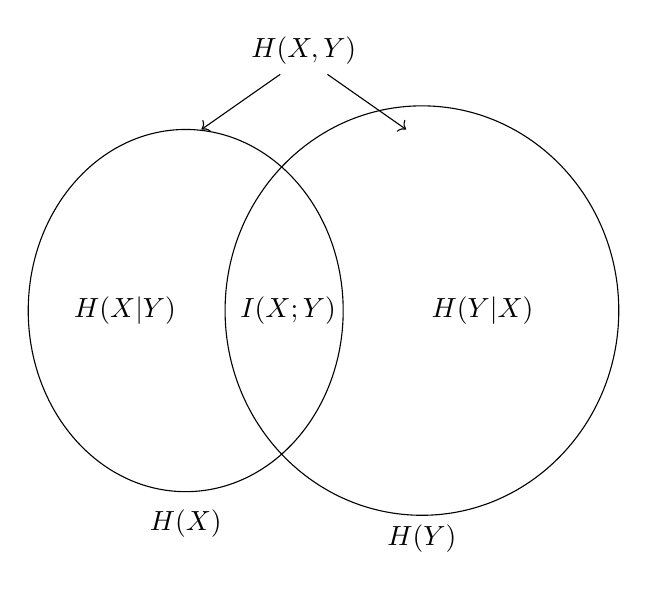
\begin{tikzpicture}
      \draw (-1.5, 0) ellipse (2 and 2.3);
      \draw (1.5, 0) ellipse (2.5 and 2.6);
      \node[left] at (-1.5,0) {$H(X|Y)$};
      \node[right] at (1.5,0) {$H(Y|X)$};
      \node[below] at (-1.5, -2.4) {$H(X)$};
      \node[below] at (1.5, -2.6) {$H(Y)$};
      \node at (-0.2, 0) {$I(X;Y)$};
      \draw[->] (-0.3, 3)--(-1.3, 2.3);
      \draw[->] (0.3,3)--(1.3, 2.3);
      \node[above] at (0,3) {$H(X, Y)$};
  \end{tikzpicture}
  \end{center}
  \end{theorem}
  \begin{proof}
  We can write
  \begin{align*}
      I(X;Y) & = \sum_{x, y} p(x, y) \, \log \frac{p(x, y)}{p(x)p(y)} \\
      & = \sum_{x, y} p(x, y) \log \frac{p(x|y)}{p(x)} \\
      & = - \sum_{x, y} p(x, y) \log p(x) + \sum_{x, y} p(x, y) \log p(x|y) \\
      & = - \sum_x p(x) \log p(x) - \Bigg( - \sum_{x, y} p(x, y) \log p(x|y) \Bigg) \\
      & = H(X) - H(X|Y)
  \end{align*}
  By symmetry, we have
  \[I(X;Y) = H(Y) - H(Y|X)\]
  Thus, $X$ says as much about $Y$ as $Y$ says about $X$. Since $H(X, Y) = H(X) + H(Y|X)$, we have
  \[I(X;Y) = H(X) + H(Y) - H(X, Y) \implies I(X;X) = H(X) - H(X|X) = H(X)\]
  That is, the mutual information of a random variable with itself is the entropy of the random variable. This is the reason that entropy is sometimes referred to as \textit{self-information}. 
  \end{proof}

  \begin{example}
  For the joint distribution in the previous example, the mutual information is 
  \[I(X;Y) = H(Y) - H(Y|X) = 2 - \frac{13}{8} = \frac{3}{8} \text{ bits}\]
  \end{example}

  \begin{definition}
  The \textbf{conditional mutual information} of random variables $X, Y, Z$ is the reduction in the uncertainty of $X$ due to knowledge of $Y$ when $Z$ is given. 
  \begin{align*}
      I(X;Y|Z) & = H(X|Z) - H(X|Y, Z) \\
      & = E_{p(x, y, z)} \bigg( \log \frac{p(X, Y|Z)}{p(X|Z) p(Y|Z)}\bigg)
  \end{align*}
  \end{definition}

  Mutual information also satisfies a chain rule. 

  \begin{theorem}[Chain rule for information]
  \[I(X_1, X_2, ..., X_n; Y) = \sum_{i=1}^n I(X_i;Y|X_{i-1}, ..., X_1)\]
  \end{theorem}
  \begin{proof}
  \begin{align*}
      I(X_1, ..., X_n;Y) & = H(X_1, ..., X_n) - H(X_1, ..., X_n |Y) \\
      & = \sum_{i=1}^n H(X_i|X_{i-1}, ..., X_1) - \sum_{i=1}^n H(X_i | X_{i-1}, ..., X_1;Y) \\
      & = \sum_{i=1}^n I(X_i ; Y|X_1, X_2, ..., X_{i-1})
  \end{align*}
  \end{proof}

  We now define a conditional version of relative entropy.

  \begin{definition}
  For joint probability mass functions $p(x, y)$ and $q(x, y)$, the \textbf{conditional relative entropy} $D\big( p(y|x) || q(y|x)\big)$ is the average of the relative entropies between the conditional probability mass functions $p(y|x)$ and $q(y|x)$ averaged over the probability mass function $p(x)$. That is, 
  \begin{align*}
      D\big(p(y|x)||q(y|x)\big) & = \sum_x p(x) \sum_y p(y|x) \, \log \frac{p(y|x)}{q(y|x)} \\
      & = \mathbb{E}_{p(x, y)} \bigg( \log \frac{p(Y|X)}{q(Y|X)} \bigg) 
  \end{align*}
  \end{definition}

  \subsection{Information Content}
  The \textbf{information content, self-information, surprisal}, or \textbf{Shannon information}, is a basic quantity derived from the probability of a particular event occurring from a random variable. It can be thought of as an alternative way of expressing probability, much like odds or log-odds, but which has particular mathematical advantages in the setting of information theory. The self-information can be interpreted as quantifying the level of "surprise" of a particular outcome. The information content can be expressed in various units of information, of which the most common is the "bit" (sometimes also called the \textit{shannon}), as explained below. 

  The definition of self-information was chosen to meet several axioms: 
  \begin{enumerate}
      \item An event with probability 100\% is perfectly unsurprising and yields no information.
      \item The less probable an event is, the more surprising it is and the more information it yields.
      \item If two independent events are measured separately, the total amount of information is the sum of the self-informations of the individual events. 
  \end{enumerate}
  It can be shown that there is a unique function of probability that meets these three axioms, up to a multiplicative scaling factor. Broadly given an event $x$ with probability $P$, the information content is defined as follows: 
  \[I(x) \equiv - \log_b \big( \mathbb{P}(x)\big)\]
  The base of the log is left unspecified, which corresponds to the scaling factor above. Formally, given a continuous random variable $X$ with probability density function $p_X (x)$, the self-information of measuring $X$ as outcome $x$ is defined as:
  \[I_X (x) \equiv - \log \big( p_X (x) \big) = \log \bigg(\frac{1}{p_X (x)}\bigg)\]

  \subsubsection{Properties}
  For a given probability space, the measurement of rarer events are intuitively more "surprising," and yield more information content, than more common values. Thus, self-information is a strictly decreasing monotonic function of the probability. While standard probabilities are represented by real numbers in the interval $[0,1]$, self-informations are represented by extended real numbers in the interval $[0,\infty]$. In particular, we have the following, for any choice of logarithmic base:
  \begin{enumerate}
      \item If a particular event has a 100\% probability of occurring, then its self-information is $-\log (1) = 0$: its occurrence is \textit{perfectly non-surprising} and yields no information.
      \item If a particular event has a 0\% probability of occurring, then its self-information is $- \log (0) = \infty$: its occurrence is \textit{infinitely surprising}.
  \end{enumerate}
  From this, we can get a few general properties: 
  \begin{enumerate}
      \item Intuitively, more information is gained from observing an unexpected event—it is \textit{surprising}.
      \item This establishes an implicit relationship between the self-information of a random variable and its variance. 
  \end{enumerate}
  Note also that this definition of information content satisfies additivity. Consider two independent random variables $X, Y$ with probability mass functions $p_X (x)$ and $p_Y (y)$ respectively. The joint probability mass function is 
  \[p_{X, Y} (x, y) \equiv \mathbb{P} (X = x, Y = y) = p_X (x) \, p_Y (y)\]
  because $X$ and $Y$ are independent. The information content of the outcome $(X, Y) = (x, y)$ is 
  \begin{align*}
      I_{X, Y} (x, y) & = - \log_2 \big( p_{X, Y} (x, y) \big) ]\\
      & = -\log_2 \big(p_X (x) \, p_Y (y)\big) \\
      & = - \log_2 \big( p_X (x) \big) - \log_2 \big( p_Y (y) \big) \\
      & = I_X (x) + I_Y (y)
  \end{align*}

  A fair coin toss, which can be measured by the Bernoulli distribution $\mathbb{P}(H) = \frac{1}{2}, \;\; \mathbb{P}(T) = \frac{1}{2}$ has the information contents (in bits, base 2) 
  \begin{align*}
      I_X (H) & = - \log_2 \big( \mathbb{P}(X = H)\big) = - \log_2 \frac{1}{2} = 1 
      I_X (T) & = - \log_2 \big( \mathbb{P}(X = T)\big) = - \log_2 \frac{1}{2} = 1 
  \end{align*}
  A fair six-sided die roll has the discrete uniform distribution. The information content is 
  \[I_X (1) = I_X (2) = I_X (3) = I_X (4) = I_X (5) = I_X (6) = -\log_2 \frac{1}{6} \approx 2.585\]
  Two independent, identically distributed dice gives an information content of 
  \[I_{X, Y} (x, y) = -\log_2 \frac{1}{36} \approx 5.169925\]
  where $1 \leq x, y \leq 6$. Note that this could have also been calculated by simply adding the self-information of one die with that of another identical die.

  \subsection{Entropy}
  The \textbf{entropy} of a random variable is the average level of \textit{information}, \textit{surprise}, or \textit{uncertainty} inherent in the variable's possible outcomes. As an example, consider a biased coin with probability p of landing on heads and probability 1-p of landing on tails. The maximum surprise is for p = 1/2, when there is no reason to expect one outcome over another, and in this case a coin flip has an entropy of one bit. The minimum surprise is when p = 0 or p = 1, when the event is known and the entropy is zero bits. Other values of p give different entropies between zero and one bits.

  Given a discrete random variable $X$, with possible outcomes $x_1, x_2, ..., x_n$ which occur with probability $P(x_1), P(x_2), ..., P(x_n)$, the entropy of $X$ is formally defined as: 
  \begin{align*}
      H(X) & \equiv - \sum_{i=1}^n \mathbb{P}(x_i) \, \log \mathbb{P}(x_i) \\
      & \equiv \mathbb{E}\big(I_X (X)\big)
  \end{align*}
  which is the expected information content of measurement of $X$. Base 2 gives the unit of bits, while base $e$ gives the \textit{natural units} nat, and base 10 gives a unit called dits. 

  The entropy was originally created by Shannon as part of his theory of communication, in which a data communication system is composed of three elements: a source of data, a communication channel, and a receiver. In Shannon's theory, the "fundamental problem of communication" – as expressed by Shannon – is for the receiver to be able to identify what data was generated by the source, based on the signal it receives through the channel. Shannon considered various ways to encode, compress, and transmit messages from a data source, and proved in his famous source coding theorem that the entropy represents an absolute mathematical limit on how well data from the source can be losslessly compressed onto a perfectly noiseless channel. 

  The English text, treated as a string of character, has fairly low entropy, i.e. is fairly predictable. If we do not know exactly what is going to come next, we can be fairly certain that, for example, 'e' will be far more common than 'z', that the combination 'qu' will be much more common than any other combination with a 'q' in it, and that the combination 'th' will be more common than 'z', 'q', or 'qu'. After the first few letters one can often guess the rest of the word. English text has between 0.6 and 1.3 bits of entropy per character of the message. 

  \subsubsection{Shannon's Source Coding Theorem}
  If a compression scheme is lossless – one in which you can always recover the entire original message by decompression – then a compressed message has the same quantity of information as the original, but communicated in fewer characters. It has more information (higher entropy) per character. A compressed message has less redundancy. Shannon's source coding theorem states a lossless compression scheme cannot compress messages, on average, to have more than one bit of information per bit of message, but that any value less than one bit of information per bit of message can be attained by employing a suitable coding scheme. The entropy of a message per bit multiplied by the length of that message is a measure of how much total information the message contains.

  This theorem establishes the limits to possible data compression. Informally, it states that 
  \begin{center}
      $N$ i.i.d. random variables each with entropy $H(X)$ can be compressed into more than $N$ $H(X)$ bits with negligible risk of information loss, as $N \rightarrow \infty$; but conversely, if they are compressed into fewer than $N$ $H(X)$ bits, it is virtually certain that information will be lost. 
  \end{center}

\section{Data Compression}

  \textbf{Data compression}, also called \textbf{source coding} or  \textbf{bit-rate reduction}, is the process of encoding information using fewer bits than the original representation. Data compression algorithms can be categorzied into two types: 
  \begin{enumerate}
      \item \textbf{Lossless compression} reduces bits by identifying and eliminating statistical redundancy. No information is lost in lossless compression. 
      \item \textbf{Lossy compression} reduces bits by removing unnecessary or less important information.
  \end{enumerate}
  Typically, a device that performs data compression is referred to as an \textbf{encoder}, and one that performs the reversal of the process (decompression) as a \textbf{decoder}. 

  A \textbf{space–time} or \textbf{time–memory trade-off} in computer science is a case where an algorithm or program trades increased space usage with decreased time. Here, space refers to the data storage consumed in performing a given task (RAM, HDD, etc), and time refers to the time consumed in performing a given task (computation time or response time). 

  A space–time trade-off can be applied to the problem of data storage. If data is stored uncompressed, it takes more space but access takes less time than if the data were stored compressed (since compressing the data reduces the amount of space it takes, but it takes time to run the decompression algorithm). Depending on the particular instance of the problem, either way is practical. There are also rare instances where it is possible to directly work (which may also be faster) with compressed data. 

  \subsection{Data Compression Ratio}
  The \textbf{data compression ratio}, also known as the \textbf{compression power}, is a measurement of the relative reduction in size of data representation produced by a data compression algorithm. It is defined as 
  \[\text{Compression Ratio} = \frac{\text{Uncompressed Size}}{\text{Compressed Size}}\]
  For example, a representation that compresses a file's storage size from 10MB to 2MB has a compression ratio of $10/2 = 5$. We can alternatively talk about the \textbf{space saving}, which is defined
  \[\text{Space Saving} = 1 - \frac{\text{Compressed Size}}{\text{Uncompressed Size}}\]
  So, the previous representation yields a space saving of 0.8, or $80\%$. 

  Lossless compression of digitized data such as video, digitized film, and audio preserves all the information, but it does not generally achieve compression ratio much better than 2:1 because of the \textbf{intrinsic entropy} of the data. Compression algorithms which provide higher ratios either incur very large overheads or work only for specific data sequences (e.g. compressing a file with mostly zeros). In contrast, lossy compression (e.g. JPEG for images, or MP3 and Opus for audio) can achieve much higher compression ratios at the cost of a decrease in quality, such as Bluetooth audio streaming, as visual or audio compression artifacts from loss of important information are introduced. In general, whether a compression ratio is high or not really depends on what kind of data is being compressed and how it is compressed. 


  \subsection{Lossless Compression}
  Lossless data compression algorithms usually exploit statistical redundancy to represent data without losing any information, so that the process is reversible. Lossless compression is possible because most real-world data exhibits statistical redundancy. For example, an image may have areas of color that do not change over several pixels; instead of coding "red pixel, red pixel, ..." the data may be encoded as "279 red pixels". This is a basic example of run-length encoding; there are many schemes to reduce file size by eliminating redundancy.

  A \textbf{dictionary coder}, also known as a \textbf{substitution coder}, is a class of lossless data compression algorithms which operate by searching for matches between the text to be compressed and a set of strings contained in a data structure (called the 'dictionary') maintained by the encoder. When the encoder finds such a match, it substitutes a reference to the string's position in the data structure. 

  Some dictionary coders use a \textit{static dictionary}, one whose full set of strings is determined before coding begins and does not change during the coding process. This approach is most often used when the message or set of messages to be encoded is fixed and large; for instance, an application that stores the contents of a book in the limited storage space of a PDA generally builds a static dictionary from a concordance of the text and then uses that dictionary to compress the verses. 

  In a related and more general method, a dictionary is built from redundancy extracted from a data environment (various input streams) which dictionary is then used statically to compress a further input stream. For example, a dictionary is built from old English texts then is used to compress a book. More common are methods where the dictionary starts in some predetermined state but the contents change during the encoding process, based on the data that has already been encoded. 

  \subsubsection{Run-length Encoding (RLE) Compression}
  RLE is a form of lossless data compression in which \textit{runs} of data (sequences in which the same data value occurs in many consecutive data elements) are stored as a single data value and count, rather than as the original run. This is most useful on data that contains many such runs.

  For example, consider a screen containing plain black text on a solid white background. There will be many long runs of white pixels in the blank space, and many short runs of black pixels within the text. A hypothetical scan line, with B representing a black pixel and W representing white, might read as follows: 
  \begin{lstlisting}
  WWWWWWWWWWWWBWWWWWWWWWWWWBBBWWWWWWWWWWWWWWWWWWWWWWWWBWWWWWWWWWWWWWW
  \end{lstlisting}
  With a RLE data compression algorithm applied to the above hypothetical scan line, it can be rendered as follows: 
  \begin{lstlisting}
  12W1B12W3B24W1B14W
  \end{lstlisting}
  which can be interpreted as a sequence of 12 Ws, 1 B, 12 Ws, 3 Bs, and so on. This run-length code represents the original 67 characters in only 18. While the actual format used for the storage of images is generally binary rather than ASCII characters like this, the principle remains the same. Even binary data files can be compressed with this method. 

\section{AON-CIRC and Straight Line Programs}

  \begin{definition}
  The most common elementary operations for algorithms are \textbf{logical operators} which can be visualized as a \textbf{gate} in a \textbf{Boolean circuit}:
  \begin{enumerate}
      \item OR: $\{0,1\}^2 \longrightarrow \{0,1\}$, defined 
      \[OR(a, b) = a \vee b = \begin{cases}
      0 & a = b = 0 \\
      1 & else
      \end{cases}\]
      An \textbf{OR gate} has two incoming wires and one (or more) outgoing wires.
      \begin{center}
      \begin{circuitikz}[scale=0.9]\draw
          (0,2) node[or port] (or) {};
      \end{circuitikz}    
      \end{center}
      \item AND: $ \{0,1\}^2 \longrightarrow \{0,1\}$, defined
      \[AND(a, b) = a \wedge b = \begin{cases}
      1 & a = b = 1 \\
      0 & else 
      \end{cases}\]
      An \textbf{AND gate} has two incoming wires and one (or more) outgoing wires. 
      \begin{center}
      \begin{circuitikz}[scale=0.9]\draw
          (0,2) node[and port] (and) {};
      \end{circuitikz}    
      \end{center}
      \item NOT: $\{0,1\} \longrightarrow \{0,1\}$, defined
      \[NOT (a) = \lnot a = \begin{cases}
      0 & a = 1 \\
      1 & a = 0
      \end{cases}\]
      A \textbf{NOT gate} has one incoming wire and one (or more) outgoing wires) 
      \begin{center}
      \begin{circuitikz}[scale=0.9]\draw
          (0,2) node[not port] (not) {};
      \end{circuitikz}    
      \end{center}
  \end{enumerate}
  \end{definition}

  Many functions can be created when composing these extremely simple functions. 

  \begin{example}
  Consider the function $MAJ: \{0,1\}^3 \longrightarrow \{0,1\}$ defined as follows
  \[MAJ (x) = \begin{cases}
  1 & x_0 + x_1 + x_2 \geq 2 \\
  0 & else
  \end{cases}\]
  We can interpret this function as the following: $MAJ(x) = 1$ if and only if there exists some pair of distinct elements $i, j$ such that both $x_i$ and $x_j$ are equal to $1$. In other words, it means that $MAJ(x) = 1$ iff \textit{either} both $x_0 = 1$ and $x_1 = 1$, \textit{or} both $x_1 = 1$ and $x_2 = 1$, \textit{or} both $x_0 = 1$ and $x_2 = 1$. Since the OR of three conditions $c_0, c_1, c_2$ can be written as
  \[OR(c_0, OR(c_1, c_2))\]
  we can now translate this function into a formula as follows: 
  \begin{align*}
      MAJ(x_0, x_1, x_2) & = OR\big( AND (x_0, x_1), OR(AND(x_1, x_2), AND(x_0, x_2)) \big) \\
      & = \big((x_0 \wedge x_1) \vee (x_1 \wedge x_2)\big) \vee (x_0 \wedge x_2)
  \end{align*}
  \end{example}

  \begin{definition}
  A \textbf{straight-line program} is a program that defines certain functions $F, G, H...$ and uses these programs to define variables of the form 
  \begin{align*}
      &\texttt{foo = F(bar,blah)} \\
      &\texttt{foo = G(bar,blah)} \\
      &\texttt{foo = H(bar)} \\
      &\texttt{... = ...}
  \end{align*}
  to come to a result. It is called a straight-line program since it contains no loops or branching (e.g. if/then statements). 

  The \textbf{AON-CIRC programming language} has the AND/OR/NOT operations defined. The binary input variables are of the form 
  \[x = (\texttt{X[0], X[1], ..., X[n-1]})\]
  and output variables of the form 
  \[y = (\texttt{Y[0], Y[1], ..., Y[m-1]})\]
  In every line, the variables on the right-hand side of the assignment operators must either be input variables or variables that have already been assigned a value. We say that an AON-CIRC program $P$ \textit{computes} a function 
  \[f: \{0,1\}^n \longrightarrow \{0,1\}^m\]
  if $P(x) = f(x)$ for every $x \in \{0,1\}^n$.
  \end{definition}

  \begin{example}
  Let the XOR function be defined
  \[XOR: \{0,1\}^2 \longrightarrow \{0,1\}, \; XOR(a, b) = a + b \pmod{2}\]
  The Boolean circuit for computing $XOR: \{0,1\}^2 \longrightarrow \{0,1\}$ is: 
  \begin{center}
  \begin{circuitikz}[scale=0.3]\draw
      (2,3) node[not port] (not1) {}
      (2,-3) node[not port] (not2) {}
      (12, 3) node[and port] (and1) {}
      (12,-3) node[and port] (and2) {}
      (18,0) node[or port] (or1) {}
      (not1.out) -- (and2.in 1)
      (not2.out) -- (and1.in 2)
      (and1.out) -- (or1.in 1)
      (and2.out) -- (or1.in 2)
      (-4,5.5) node(a) {X[0]}
      (-4,-5.5) node(b) {X[1]}
      (a) -- (not1.in)
      (b) -- (not2.in)
      (a) -- (and1.in 1)
      (b) -- (and2.in 2)
      (21,0) node(y) {Y[0]}
      (or1.out)--(y);
  \end{circuitikz}
  \end{center}
  This can be computed with the straight-line algorithm as such. Given $(a, b)$ as inputs, we have $w_1 = AND(a, b), w_2 = NOT(w_1)$, and $w_3 = OR(a, b)$. Then the algorithm returns $AND(w_2, w_3)$. In Python, this can be programmed: 
  \begin{lstlisting}
  def AND(a, b): return a*b
  def OR(a, b): return 1-(1-a)*(1-b)
  def NOT(a): return 1-a

  def XOR(a, b): 
      w1 = AND(a, b)
      w2 = NOT(w1)
      w3 = OR(a,b)
      return AND(w2, w3)

  print([f"XOR({a},{b})={XOR(a,b)}" for a in [0,1] for b in [0,1]])
  # ['XOR(0,0)=0', 'XOR(0,1)=1', 'XOR(1,0)=1', 'XOR(1,1)=0']
  \end{lstlisting}
  \end{example}



  Note that Boolean circuits are a \textit{mathematical model} that does not necessarily correspond to a physical object, but they can be implemented physically. In physical implementation of circuits, the signal is often implemented by electric potential, or voltage, on a wire, where for example voltage above a certain level is interpreted as a logical value of $1$, and below a certain level is interpreted as a logical value of $0$. Furthermore, the way that we've presented the XOR function through Boolean circuits and straight-line programs hints at the following: 

  \begin{theorem}[Equivalence of circuits and straight line programs]
  Let $f: \{0,1\}^n \longrightarrow \{0,1\}^m$ and $s \geq m$ be some number. Then $f$ is computable by a Boolean circuit of $s$ gates if and only if $f$ is computable by an AON-CIRC program of $s$ lines. 
  \end{theorem}

  \begin{example}
  Let us define the function $ALLEQ: \{0,1\}^4 \longrightarrow \{0,1\}$ to be the function that on input $x \in \{0,1\}^4$ outputs $1$ if and only if $x_0 = x_1 = x_2 = x_3$. The Boolean circuit for computing ALLEQ is: 
  \begin{center}
  \begin{circuitikz}[scale=0.4]\draw
      (2, 2) node[and port] (and1) {}
      (2, 6) node[not port] (not1) {}
      (2, 10) node[not port] (not2) {}
      (8, 2) node[and port] (and2) {}
      (8, 6) node[and port] (and3) {}
      (8, -2) node[not port] (not3) {}
      (14, 6) node[and port] (and4) {}
      (14, 10) node[and port] (and5) {}
      (14, 14) node[not port] (not4) {}
      (19.5, 12) node[and port] (and6) {}
      (24, 11) node[or port] (or1) {}
      (-4,-1) node(d) {X[3]}
      (-4, 3) node(c) {X[2]}
      (-4, 8) node(b) {X[1]}
      (-4, 12) node(a) {X[0]}
      (a)--(not4.in)
      (a)--(and5.in 1)
      (b)--(not2.in)
      (b)--(and1.in 1)
      (c)--(not1.in) 
      (c)--(and1.in 2)
      (d)--(and2.in 2)
      (d)--(not3.in) 
      (and1.out)--(and2.in 1)
      (not1.out)--(and3.in 2)
      (not2.out)--(and3.in 1)
      (and2.out)--(and5.in 2) 
      (and3.out)--(and4.in 1) 
      (and4.out)--(and6.in 2) 
      (not3.out)--(and4.in 2) 
      (and5.out)--(or1.in 2) 
      (not4.out)--(and6.in 1)
      (and6.out)--(or1.in 1)
      (26, 11) node(y) {Y[0]}
      (or1.out)--(y);
  \end{circuitikz}
  \end{center}
  \end{example}

  \subsection{Topological Sortings of Graphs}
  We now proceed to formally define Boolean circuits. But first, we must cover a few prerequisite definitions: 

  \begin{definition}[Directed Graphs]
  A \textbf{directed graph} $G = (V, E)$ consists of a set $V$ and a set $E \subseteq V \times V$ of ordered pairs of $V$, which denotes the edge $(u, v)$ or also as $u \rightarrow v$. If the edge $u \rightarrow v$ is present in the graph, then $v$ is called an \textbf{out-neighbor} of $u$ and $u$ is an \textbf{in-neighbor} of $v$. 

  The \textbf{in-degree} of $u$ is the number of in-neighbors it has, and the \textbf{out-degree} of $v$ is the number of out-neighbors it has. A \textbf{path} in the graph is a tuple $(u_0, u_1, ..., u_k) \in V^{k+1}$ for some $k > 0$ such that $u_{i+1}$ is an out-neighbor of $u_i$ for every $i \in [k]$. A \textit{simple path} is a path $(u_0, ..., u_k)$ where all the $u_i$'s are distinct, and a \textit{cycle} is a path where $u_0 = u_k$. 
  \end{definition}

  \begin{definition}[Directed Acyclic Graphs]
  We say that $G = (V, E)$ is a \textbf{directed acyclic graph (DAG)} if it is a directed graph and there does not exist a list of vertices $u_0, u_1, ... u_k \in V$ such that $u_0 = u_k$ and for every $i \in [k]$, the edge $u_i \rightarrow u_{i+1}$ is in $E$. 
  \end{definition}

  Every directed acyclic graph can be arranged in layers so that for all directed edges $u \rightarrow v$, the layer of $v$ is larger than the layer of $u$. This is expressed more formally in the following definition. 

  \begin{definition}[Layering of a DAG]
  Let $G = (V, E)$ be a directed graph. A \textbf{layering} of $G$ is a function 
  \[f: V \longrightarrow \mathbb{N}\]
  such that for every edge $u \rightarrow v$, $f(u) < f(v)$.
  \end{definition}

  The next lemma is extremely useful. 
  \begin{theorem}
  Let $G$ be directed graph. Then $G$ is acyclic if and only if there exists a layering $f$ of $G$. This is result is known as \textbf{topological sorting}. 
  \end{theorem}

  \begin{corollary}
  There exists a layering for every directed acyclic graph. That is, every DAG can be topologically sorted. 
  \end{corollary}

  \subsubsection{Formal Definition of Boolean Circuits}
  \begin{definition}
  Let $n, m, s$ be positive integers with $s \geq m$. A \textbf{Boolean circuit} with $n$ inputs, $m$ outputs, and $s$ gates, is a labeled \textit{directed acyclic graph} (DAG) 
  \[G = (V, E)\]
  with $s+n$ vertices satisfying the following properties: 
  \begin{enumerate}
      \item Exactly $n$ of the vertices have no in-neighbors (i.e. inputs). These vertices known known as \textbf{inputs} and are labeled with the $n$ labels
      \[X[0], X[1], ..., X[n-1]\]
      Each input has at least one out-neighbor. 
      \item The other $s$ vertices are known as \textbf{gates}. Each gate is labeled with $\wedge, \vee$, or $\lnot$. Gates labeled with $\wedge$ (AND) or $\vee$ (OR) have two in-neighbors. Gates labeled with $\lnot$ (NOT) have one in-neighbor. \textbf{Parallel edges} are allowed. 
      \item Exactly $m$ of the gates are also labeled with the $m$ labels 
      \[Y[0], Y[1], ..., Y[m-1]\]
      in addition to their label $\wedge$/$\vee$/$\lnot$. These are known as \textbf{outputs}. 
  \end{enumerate}
  The \textbf{size} of a Boolean circuit is the number of gates it contains. 
  \end{definition}
  Having parallel edges means that an AND or OR gate $u$ can have both its in-neighbors be the same gate $v$. Since $AND(a, a) = OR(a, a) = a$ for every $a \in \{0,1\}$, such parallel gates don't help in computing new values in circuits with AND/OR/NOT gates.
  \begin{center}
  \begin{circuitikz}\draw
      (0, 0) node[and port] (and1) {}
      (5,0) node[and port] (and2) {}
      (and1.out)--(and2.in 1)
      (and1.out)--(and2.in 2)
      ;
  \end{circuitikz}
  \end{center}

  We clarify the definition with the previous example of the function ALLEQ. 
  \begin{center}
  \begin{circuitikz}[scale=0.4]\draw
      (2, 2) node[and port] (and1) {}
      (2, 6) node[not port] (not1) {}
      (2, 10) node[not port] (not2) {}
      (8, 2) node[and port] (and2) {}
      (8, 6) node[and port] (and3) {}
      (8, -2) node[not port] (not3) {}
      (14, 6) node[and port] (and4) {}
      (14, 10) node[and port] (and5) {}
      (14, 14) node[not port] (not4) {}
      (19.5, 12) node[and port] (and6) {}
      (24, 11) node[or port] (or1) {}
      (-4,-1) node(d) {X[3]}
      (-4, 3) node(c) {X[2]}
      (-4, 8) node(b) {X[1]}
      (-4, 12) node(a) {X[0]}
      (a)--(not4.in)
      (a)--(and5.in 1)
      (b)--(not2.in)
      (b)--(and1.in 1)
      (c)--(not1.in) 
      (c)--(and1.in 2)
      (d)--(and2.in 2)
      (d)--(not3.in) 
      (and1.out)--(and2.in 1)
      (not1.out)--(and3.in 2)
      (not2.out)--(and3.in 1)
      (and2.out)--(and5.in 2) 
      (and3.out)--(and4.in 1) 
      (and4.out)--(and6.in 2) 
      (not3.out)--(and4.in 2) 
      (and5.out)--(or1.in 2) 
      (not4.out)--(and6.in 1)
      (and6.out)--(or1.in 1)
      (26, 11) node(y) {Y[0]}
      (or1.out)--(y);
      \draw[color=blue] (-5, -4) rectangle (-3, 16);
      \node[color=blue, above] at (-4, 16) {n Inputs};
      \draw[color=red] (-2, -4) rectangle (25, 16); 
      \node[color=red, above] at (10,16) {s Gates};
      \draw[color=teal] (20.5, 8.5) rectangle (24.5, 13);
      \node[color=teal, below] at (20, 8.5) {m Outputs (Gates)};
      \node at (18, 5) {$s \geq m$};
  \end{circuitikz}
  \end{center}

  \begin{definition}
  We can also see that a Boolean circuit naturally induces a function defined in the space $\{0,1\}^n$. That is, given Boolean circuit $C$ with $n$ inputs and $m$ outputs, let the \textit{output} of $C$ on the input $x \in \{0,1\}^n$ be denoted $C(x)$. Then, if a function
  \[f: \{0,1\}^n \longrightarrow \{0,1\}^m\]
  satisfies $f(x) = C(x)$ for all $x \in \{0,1\}^n$, we say that the circuit $C$ \textbf{computes} $f$. 
  \end{definition}

  \subsection{Physical Implementations of Computing Devices}
  Note that \textit{computation} is an abstract notion (a process) that is distinct from its physical \textit{implementations} (how the progress is run). While most modern computing devices are obtained by mapping logical gates to semiconductor-based transistors, throughout history people have computed using a huge variety of mechanisms, including mechanical systems, gas and liquid (known as fluidics), biological and chemical processes, and even living creatures. We will explore some ways that allow us to directly translate Boolean circuits to the physical world, without going through the entire stack of architecture, operating systems, and compilers. 

  \subsubsection{Transistors}
  A transistor can be thought of as an electric circuit with two inputs, known as the source and the gate and an output, known as the sink. The gate controls whether current flows from the source to the sink. In a standard transistor, if the gate is “ON” then current can flow from the source to the sink and if it is “OFF” then it can’t. In a complementary transistor this is reversed: if the gate is “OFF” then current can flow from the source to the sink and if it is “ON” then it can’t. 

  We can use transistors to implement various Boolean functions such as and AND, OR, and NOT. For each a two-input gate $G: \{0,1\}^2 \longrightarrow \{0,1\}$, such an implementation would be a system with two input wires $x, y$ and one output wire $z$, such that if we identify high voltage with $1$ and low voltage with $0$, then the wire $z$ will equal to $1$ if and only if applying $G$ to the values of the wires $x$ and $y$ is $1$. 

  \textbf{Biological computing} Computation can be based on biological or chemical systems. For example the lac operon produces the enzymes needed to digest lactose only if the conditions $x \wedge (\lnot y)$ hold, where $x$ is "lactose is present" and $y$ is "glucose is present." 


  \textbf{Cellular Automata and the Game of Life} Cellular automata is a model of a system composed of a sequence of cells, each of which can have a finite state. At each step, a cell updates its state based on the states of its neighboring cells and some simple rules. As we will discuss later in this book, cellular automata such as Conway’s \textit{Game of Life} can be used to simulate computation gates .

  \textbf{Neural Networks} Another computation device is the brain. Even though the exact working of the brain is still not fully understood, one common mathematical model for it is a (very large) \textbf{neural network}. 

  A neural network can be thought of as a Boolean circuit that instead of AND/OR/NOT uses some other gates as the basic basis. One particular basis we can use are \textbf{threshold gates}. For every vector
  \[w = (w_0, w_1, ..., w_{k-1})\]
  of integers and integer $t$ (some or all of which could be negative), the \textbf{threshold function corresponding to $w, t$} is the function $T_{w, t} :\{0,1\}^k \longrightarrow \{0,1\}$ that maps $x \in \{0,1\}^k$ to $1$ if and only if
  \[\sum_{i=0}^{k-1} w_i x_i \geq t\]
  that make up the core of human and animal brains. To a first approximation, a neuron has $k$ inputs and a single output, and the neurons “fires” or “turns on” its output when those signals pass some threshold. 

  \subsection{The NAND Function}
  \begin{definition}
  The NAND function is a function mapping $\{0,1\}^2$ to $\{0,1\}$ defined by
  \[NAND(a, b) = \begin{cases}
  0 & a = b = 1 \\
  1 & else
  \end{cases}\]
  NAND is really the composition of the NOT and AND functions; that is, 
  \[NAND(a, b) = (NOT \circ AND) (a, b)\]
  \end{definition}

  Here is an interesting result. 

  \begin{theorem}[Universality of NAND]
  We can compute AND, OR, and NOT by composing only the NAND function. 
  \end{theorem}
  \begin{proof}
  We can see that, using double negation, 
  \begin{align*}
      NOT(a) & = NOT(AND(a, a)) \\
      & = NAND(a, a)\\
      AND(a, b) & = NOT(NOT(AND(a, b))) \\
      & = NOT(NAND(a, b)) \\
      & = NAND(NAND(a, b), NAND(a, b)) \\
      OR(a, b) & = NOT(AND(NOT(a), NOT(b))) \\
      & = NOT(AND(NAND(a,a), NAND(b,b))) \\
      & = NAND(NAND(a, a), NAND(b, b)) 
  \end{align*}
  \end{proof}

  \begin{corollary}
  For every Boolean circuit $C$ of $s$ gates, there exists a NAND circuit $C^\prime$ of at most $3s$ gates that computes the same function as $C$. 
  \end{corollary}
  \begin{proof}
  Replace every AND, OR, and NOT gate with their NAND equivalents. 
  \end{proof}

  \subsubsection{NAND Circuits}

  \begin{definition}
  A \textbf{NAND Circuit} is a circuit in which all the gates are NAND operations. Despite their simplicity, NAND circuits can be quite powerful. 
  \end{definition}

  \begin{example}
  We can create a NAND circuit of the XOR function that maps $x_0, x_1 \in \{0,1\}$ to $x_0 + x_1 \pmod{2}$. 
  \begin{center}
  \begin{circuitikz}[scale=0.4]\draw
      (0,0) node[nand port] (nand1) {}
      (5, 2) node[nand port] (nand2) {}
      (5, -2) node[nand port] (nand3) {}
      (10,0) node[nand port] (nand4) {}
      (nand1.out)--(nand2.in 2)
      (nand1.out)--(nand3.in 1)
      (nand2.out)--(nand4.in 1)
      (nand3.out)--(nand4.in 2) 
      (-6, 3) node(x1) {X[0]}
      (-6, -3) node(x2) {X[1]}
      (x1)--(nand1.in 1)
      (x2)--(nand1.in 2)
      (x1)--(nand2.in 1)
      (x2)--(nand3.in 2)
      (13,0) node(y) {Y[0]}
      (nand4.out)--(y)
      ;
  \end{circuitikz}
  \end{center}
  \end{example}

  \begin{definition}
  Two models are said to be \textit{equivalent in power} if they can be used to compute the same set of functions. 
  \end{definition}

  Just as we have defined the AON-CIRC program, we can define the notion of computation by a NAND-CIRC program in the natural way. 

  \begin{theorem}[Equivalence between models of finite computation]
  For every sufficiently large $s, n, m$ and $f: \{0,1\}^n \longrightarrow \{0,1\}^m$, the following conditions are all equivalent to one another: 
  \begin{enumerate}
      \item $f$ can be computed by a Boolean circuit (with $\wedge, \vee, \lnot$ gates) of at most $O(s)$ gates. 
      \item $f$ can be computed by an AON-CIRC straight-line program of at most $O(s)$ lines
      \item $f$ can be computed by a NAND circuit of at most $O(s)$ gates. 
      \item $f$ can be computed by a NAND-CIRC straight-line program of at most $O(s)$ lines. 
  \end{enumerate}
  By $O(s)$, we mean that the bound is at most $c \cdot s$, where $c$ is a constant that is independent of $n$. For example, if $f$ can be computed by a Boolean circuit of $s$ gates, then it can be computed by a NAND-CIRC program of at most 3$s$ lines, and if $f$ can be computed by a NAND circuit of $s$ gates, then it can be computed by an AON-CIRC program of at most $2s$ lines. 
  \end{theorem}

  \subsubsection{Circuits with other Gate Sets}
  We can expand beyond the basis functions of AND/OR/NOT or NAND to a general set of functions 
  \[\mathcal{G} = \{G_0, G_1, ..., G_{k-1}\}\]
  With this, we can define a notion of circuits that use elements of $\mathcal{G}$ as gates and a notion of a \textit{$\mathcal{G}$ programming language} where every line involves assigning to a variable $\texttt{foo}$ the result of applying some $G_i \in \mathcal{G}$ to previously defined or input variables. We state this formally. 

  \begin{definition}[General Straight-line programs]
  Let $\mathcal{F} = \{f_0, f_1, ..., f_{t-1}\}$ be a finite collection of Boolean functions such that
  \[f_i: \{0,1\}^k \longrightarrow \{0,1\}\]
  for some $k_i \in \mathbb{N}$. A \textbf{$\mathcal{F}$ program} is a sequence of lines, each of which assigns to some variable the result of applying some $f_i \in \mathcal{F}$ to $k_i$ other variables. As above, we use $\texttt{X[i]}$ and $\texttt{Y[j]}$ to denote the input and output variables. 

  We say that $\mathcal{F}$ is a \textbf{universal set of operations} (or a \textbf{universal gate set}) if there exists a $\mathcal{F}$ program to compute the function NAND. 
  \end{definition}

  \begin{example}
  Let $\mathcal{F} = \{IF, ZERO, ONE\}$ where 
  \[ZERO: \{0,1\} \longrightarrow \{0\}, \;\; ONE: \{0,1\} \longrightarrow \{1\}\]
  are the constant zero and one functions, and 
  \[IF: \{0,1\}^3 \longrightarrow \{0,1\}, \; IF (a, b, c) = \begin{cases}
  b & a = 1 \\
  c & else 
  \end{cases}\]
  Then, $\mathcal{F}$ is universal since we can use the following formula to compute NAND: 
  \[NAND(a, b) = IF\big( a, IF(b, ZERO, ONE), ONE\big)\]
  \end{example}

  There are some sets $\mathcal{F}$ that are more restricted in power. For example, it can be shown that if we use only AND or OR gates (without NOT), then we do not get an equivalent model of computation. 

  \subsection{Syntactic Sugar}
  Just as we have built the AND, OR, and NOT gates with the NAND gate, we can implement more complex features using our basic building blocks, and then use these new features themselves as building blocks for even more sophisticated features. This is known as \textbf{syntactic sugar}, since we are not modifying the underlying programming model itself, but rather we merely implement new features by syntactically transforming a program that uses such features into one that doesn’t. It makes the language "sweeter" for human use: things can be expressed more clearly, more concisely, or in an alternative style that some may prefer.

  In computer programming, we can define and then execute \textbf{procedures} or \textbf{subroutines}, which are often known as \textit{functions}. 

  \begin{example}
  We can use syntactic sugar to compute the majority function MAJ as follows, by first defining the procedures NOT, AND, and OR. 
  \begin{lstlisting}
  def NOT(a):
  return NAND(a,a)
  def AND(a,b):
  temp = NAND(a,b) return NOT(temp)
  def OR(a,b):
  temp1 = NOT(a)
      temp2 = NOT(b)
      return NAND(temp1,temp2)
      def MAJ(a,b,c): and1 = AND(a,b)
      and2 = AND(a,c) and3 = AND(b,c)
      or1 = OR(and1,and2) return OR(or1,and3)

  print(MAJ(0,1,1))
  # 1
  \end{lstlisting}
  \end{example}

  Note that compared to writing out the full Boolean circuit without any syntactic sugar, one with sugar will can be much simpler. It's the difference between having access to only NAND, or all of NAND, AND, OR, NOT. 

  \begin{definition}
  We call these the programming language NAND-CIRC augmented with the syntax above (for defining procedures) a \textbf{NAND-CIRC-PROC} program. Note that NAND-CIRC-PROC only allows \textit{non-recursive} procedures (that is, procedures that take in its return value as its argument). 
  \end{definition}

  Since the procedures are defined using the NAND operator, it is trivial that for every NAND-CIRC-PROC program $P$, there exists a "sugar-free" NAND-CIRC program $P^\prime$ that computes the same function as $P$. 

  \subsubsection{Conditional Statements}
  We can define conditional (if/then) statements using NAND operators. The idea is to compute the function $IF: \{0,1\}^3 \longrightarrow \{0,1\}$ such that $IF(a, b, c)$ equals $b$ if $a = 1$ and $c$ if $a = 0$. 

  \begin{definition}
  The IF function can be implemented from NANDs as follows: 
  \begin{lstlisting}
  def IF(cond, a, b);
      notcond = NAND(cond, cond) 
      temp = NAND(b, notcond)
      temp1 = NAND(a, cond)
      return NAND(temp, temp1)
  \end{lstlisting}
  The IF function is also known as a multiplexing function, since $cond$ can be thought of as a switch that controls whether the output is connected to $a$ or $b$. 
  \end{definition}

  With this, we can replace code of the form 
  \begin{lstlisting}
  if (condition): assign blah to variable foo
  \end{lstlisting}
  with code of the form 
  \begin{lstlisting}
  foo = IF(condition, blah, foo) 
  \end{lstlisting}
  that assigns to $\texttt{foo}$ its old value when $\texttt{condition}$ equals $0$, and assign to $\texttt{foo}$ the value of $\texttt{blah}$ otherwise.

  \begin{definition}
  Let NAND-CIRC-IF be the programming language NAND-CIRC augmented with $\texttt{if/then/else}$ statements for allowing code to be conditionally executed based on whether a variable is equal to $0$ or $1$. 
  \end{definition}

  \begin{theorem}
  For every NAND-CIRC-IF program $P$, there exists a standard (i.e. "sugar-free") NAND- CIRC program $P^\prime$ that computes the same function as $P$. 
  \end{theorem}

  \subsubsection{Addition and Multiplication}
  We can write the integer addition function as follows: 
  \begin{lstlisting}
  # Add two n-bit integers
  # Use LSB first notation for simplicity 
  def ADD(A,B):
      Result = [0]*(n+1) 
      Carry = [0]*(n+1) 
      Carry[0] = zero(A[0]) 
      for i in range(n):
          Result[i] = XOR(Carry[i],XOR(A[i],B[i]))
          Carry[i+1] = MAJ(Carry[i],A[i],B[i]) Result[n] = Carry[n]
      return Result
      
  ADD([1,1,1,0,0],[1,0,0,0,0]);; 
  # [0, 0, 0, 1, 0, 0]
  \end{lstlisting}
  where $\texttt{zero}$ is the zero function, and $\texttt{MAJ, XOR}$ correspond to the majority and XOR functions respectively. Note that in here, $n$ is a \textit{fixed integer} and so for every such $n$, $\texttt{ADD}$ is a \textit{finite} function that takes as input $2n$ bits and outputs $n+1$ bits. Note that the $\texttt{for}$ loop isn't anything fancy at all; it is just shorthand notation of simply repeating the code $n$ times. By expanding out all the features, for every value of $n$ we can translate the above program into a standard ("sugar-free") NAND-CIRC program. Note that the sugar free NAND-CIRC program to adding two-digit binary numbers consists of 43 lines of code, with a Boolean circuit of 15 layers. 

  We can in fact prove the following theorem that gives an upper bound on the addition algorithm. 

  \begin{theorem}[Addition using NAND-CIRC programs]
  For every $n \in \mathbb{N}$, let 
  \[ADD_n : \{0,1\}^{2n} \longrightarrow \{0,1\}^{n+1}\]
  be the function that, given $x, x^\prime \in \{0,1\}^n$, computes the representation of the sum of the numbers that $x$ and $x^\prime$ represent. Then, for every $n$ there is a NAND-CIRC program to compute $ADD_n$ with at most $9n$ lines. 
  \end{theorem}

  Once we have addition, we can use grade-school algorith of multiplication to obtain multiplication as well. 

  \begin{theorem}[Muliplication using NAND-CIRC programs]
  For every $n$, let 
  \[MULT_n : \{0,1\}^{2n} \longrightarrow \{0,1\}^{2n}\]
  be the function that, given $x, x^\prime \in \{0,1\}^n$, computes the representation of the product of the numbers that $x$ and $x^\prime$ represent. Then, there is a constant $c$ such that for every $n$, there is a NAND-CIRC program of at most $cn^2$ that computes the function $MULT_n$. 
  \end{theorem}

  The \textit{Karatsuba's algorithm} allows us to actually compute that there is a NAND-CIRC program of $O(n^{\log_2 3})$ lines to compute $MULT_n$. 

  \subsubsection{The Lookup Function}
  The LOOKUP function tells us the value of a certain entry. 
  \begin{definition}[Lookup function]
  For every $k$, the \textbf{lookup function} of order $k$, 
  \[LOOKUP_k: \{0,1\}^{2^k} \times \{0,1\}^k \simeq \{0,1\}^{2^k + k} \longrightarrow \{0,1\}\]
  (where $\simeq$ denotes isomorphism) is defined as follows: For every $x \in \{0,1\}^{2^k}$ and $i \in \{0,1\}^k$, 
  \[LOOKUP_k (x, i) = x_i\]
  where $x_i$ denotes the $i$th entry of $x$ in binary representation. 
  \end{definition}

  \begin{theorem}
  For every $k > 0$, there is a NAND-CIRC program that computes the function $LOOKUP_k: \{0,1\}^{2^k + k} \longrightarrow \{0,1\}$. The number of lines in this program is at most $4 \cdot 2^k$. This also means that $LOOKUP_k$ can be computed by a Boolean circuit (with AND, OR, and NOT) gates of at most $8 \cdot 2^k$ gates. 
  \end{theorem}

  \subsubsection{Computing Every Function}

  In fact, we can compute \textit{every} finite function with a large enough Boolean (or equivalently, NAND) circuit. 

  \begin{theorem}[Universality of Finite Functions]
  There exists some constant $c > 0$ such that for every $n, m > 0$ and function
  \[f: \{0,1\}^n \longrightarrow \{0,1\}^m\]
  there is a NAND-CIRC program/NAND circuit,  with at most $c \cdot m 2^n$ lines/gates that computes the function $f$. 
  \end{theorem}

  Since the models of NAND circuits, NAND-CIRC programs, and AON-CIRC programs, and Boolean circuits are all equivalent to one another, we can restate the theorem as such. 

  This may not be so surprising actually. After all, a finite function $f: \{0,1\}^n \longrightarrow \{0,1\}^m$ can be represented by simply the list of its outputs for each one of the $2^n$ input values. So it makes sense that we could write a NAND-CIRC program of similar size to compute it. 

  \begin{definition}
  For every $n, m \in \{1, 2, ..., 2s\}$, let $SIZE_{n, m} (s)$ denote the set of all functions $f: \{0,1\}^n \longrightarrow \{0,1\}^m$ such that $f \in SIZE(s)$. We denote $SIZE_n (s)$ to be just $SIZE_{n,1} (s)$. For every integer $s \geq 1$, we let 
  \[SIZE(s) = \bigcup_{n, m \leq 2s} SIZE_{n, m} (s)\]
  be the set of all functions $f$ that can be computed by NAND circuits of at most $s$ gates (or equivalently, by NAND-CIRC programs of at most $s$ lines). 
  \end{definition}

  We can summarize the equivalence of these models below: 
  \begin{center}
  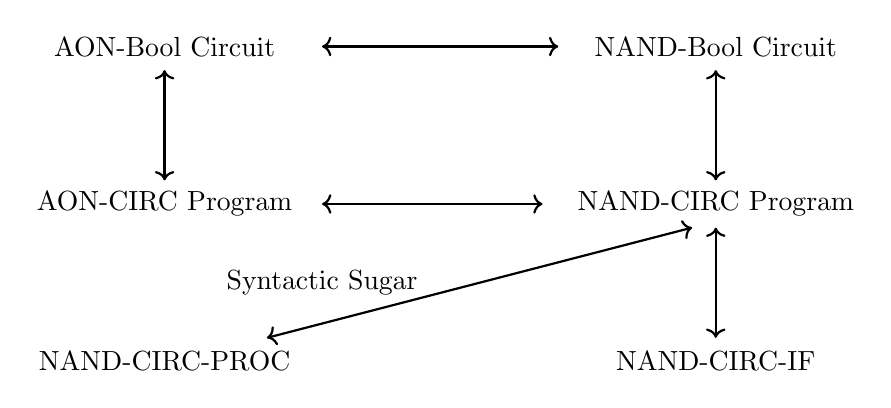
\begin{tikzpicture}
      \node at (0, 0) {AON-Bool Circuit};
      \node at (0, -2) {AON-CIRC Program};
      \node at (7, 0) {NAND-Bool Circuit};
      \node at (7, -2) {NAND-CIRC Program};
      \node at (0, -4) {NAND-CIRC-PROC};
      \node at (7, -4) {NAND-CIRC-IF};
      \draw[<->, thick] (0, -0.3)--(0, -1.7);
      \draw[<->, thick] (7, -0.3)--(7, -1.7);
      \draw[<->, thick] (7, -2.3)--(7, -3.7);
      \draw[<->, thick] (2, 0)--(5,0);
      \draw[<->, thick] (2, -2)--(4.8,-2);
      \draw[<->, thick] (6.7, -2.3)--(1.3, -3.7);
      \node at (2, -3) {Syntactic Sugar};
  \end{tikzpicture}
  \end{center}

\section{Code as Data, Data as Code}

  A program is simply a sequence of symbols, each of which can be encoded in binary using (for example) the ASCII standard. Therefore, we can represent every NAND-CIRC program (and hence also every Boolean circuit) as a binary string. This means that we can treat circuits or NAND-CIRC programs both as instructions to carrying computation and also as \textit{data} that could potentially be used as \textit{inputs} to other computations. That is, \textbf{a program is a piece of text, and so it can be fed as input to other programs}. 

  \subsection{Representing Programs as Strings}
  We can represent programs or circuits as strings in many ways. For example, since Boolean circuits are labeled directed acyclic graphs, we can use the \textit{adjacency matrix} representations. A simpler way is to just interpret the program as a sequence of letters and symbols. For example, the NAND-CIRC program $P$: 
  \begin{lstlisting}
  temp_0 = NAND(X[0],X[1])
  temp_1 = NAND(X[0],temp_0)
  temp_2 = NAND(X[1],temp_0)
  Y[0] = NAND(temp_1,temp_2)
  \end{lstlisting}
  is simply a string of 107 symbols which include lower and upper case letters, digits, the underscore character, equality signs, punctuation marks, space, and the "new line" markers, all of which can be encoded in ASCII. Since every symbol can be encoded as a string of $7$ bits using the ASCII encoding, the program $P$ can be encoded as a string of length $7 \cdot 107 = 749$ bits. Therefore, we can prove that \textit{every} NAND-CIRC program can be represented as a string in $\{0,1\}^*$. 

  Furthermore, since the names of the working variables of a NAND-CIRC program do not affect its functionality, we can always transform a program to have the form of $P^\prime$, where all variables apart from the inputs and outputs, have the form $\texttt{temp}_0$, $\texttt{temp}_1$, ... Moreover, if the program has $s$, lines, then we will never need to use an index larger than $3s$ (since each line involves at most three variables), and similarly, the indices of the input and output variables will all be at most $3s$. Since a number between $0$ and $3s$ can be expressed using at most $\left\lceil{\log_{10} (3s+1)} \right\rceil = O(\log s)$ digits, each line in the program (which has the form $\texttt{foo = NAND(bar, blah)}$), can be represented using $O(1) + O(\log s) = O(\log s)$ symbols, each of which can be represented by $7$ bits. This results in the following theorem 

  \begin{theorem}[Representing programs as strings]
  There is a constant $c$ such that for $f \in SIZE(s)$, there exists a program $P$ computing $f$ whose string representation has length at most $cs \log s$. 
  \end{theorem}

  \subsection{Counting Programs}
  We can actually see that the number of programs of certain length is bounded by the number of strings that represent them. 

  \begin{theorem}[Counting programs]
  For every $s \in \mathbb{N}$, 
  \[|SIZE(s)| \leq 2^{O(s \log s)}\]
  That is, there are at most $2^{O (s \log s)}$ functions computed by NAND-CIRC programs of at most $s$ lines. This gives a limitation on NAND-CIRC programs running on at most a given number of $s$ lines. 
  \end{theorem}

  Note that a function mapping $\{0,1\}^2 \longrightarrow \{0, 1\}$ can be identified with a table of its four values on the inputs 00, 01, 10, 11. A function mapping $\{0,1\}^3 \longrightarrow \{0,1\}$ can be identified with the table of its 8 values on the inputs 000, 001, 010, 011, 100, 101, 110, 111. More generally, every function 
  \[F: \{0,1\}^n \longrightarrow \{0,1\}\]
  is equal to the number of such tables which is $2^{2^n}$. Note that this is a \textit{double exponential} in $n$, and hence even form small values of $n$ (e.g. $n = 10$), the number of functions from $\{0,1\}^n \longrightarrow \{0,1\}$ is large. 

  \begin{theorem}[Counting argument lower bound]
  The shortest NAND-CIRC program to compute $f: \{0,1\}^n \longrightarrow \{0,1\}$ requires more than $\delta \cdot 2^n / n$ lines. That is, there exists a constant $\delta > 0$ such that for every sufficiently large $n$, there exists $f: \{0,1\}^n \longrightarrow \{0,1\}$ such that $f \not\in SIZE\Big( \frac{\delta 2^n}{n}\Big)$. The constant $\delta$ can be proven to be arbitrarily close to $\frac{1}{2}$. 
  \end{theorem}

  We already know that every function mapping $\{0,1\}^n$ to $\{0,1\}$ can be computed by an $O(2^n / n)$ line program. The previous theorem shows that some functions do require an astronomical number of lines to compute. That is, \textbf{some functions $f: \{0,1\}^n \longrightarrow \{0,1\}$ cannot be computed by a Boolean circuit using fewer than exponential (in $n$) number of gates}. 

  \subsection{Tuples Representation}
  ASCII is a fine representation of programs, but we can do better. That is, give a NAND-CIRC program with lines of the form 
  \begin{lstlisting}
  blah = NAND(baz, boo)
  \end{lstlisting}
  We can encode each line as the triple $\texttt{(blah, baz, boo)}$. Furthermore, we can associate each variable with a number and encode the line with the 3-tuple $(i, j, k)$. Expanding on this, we can associate every variable with a number in the set
  \[[t] = \{0, 1, 2, ..., t-1\}\]
  where the first $n$ numbers $\{0, ..., n-1\}$ correspond to input variable, the last $m$ numbers $\{t-m, ..., t-1\}$ correspond to the output variables, and the intermediate numbers $\{n, ..., t-m-1\}$ correspond to the remaining variables. 

  \begin{definition}[List of tuples representation]
  Let $P$ be a NAND-CIRC program of $n$ inputs, $m$ outputs, and $s$ lines, and let $t$ be the number of distinct variables used by $P$. The \textbf{list of tuples representation of $P$} is the triple $(n, m, L)$, where $L$ is the list of triples of the form $(i, j, k)$ for $i, j, k \in [t]$. We assign a number for a variable of $P$ as follows:
  \begin{enumerate}
      \item For every $i \in [n]$, the variable $\texttt{X[i]}$ is assigned to the number $i$. 
      \item For every $j \in [m]$, the variable $\texttt{Y[j]}$ is assigned to the number $t - m + j$.
      \item Every other variable is assigned a number in $\{n, n+1, ..., t-m-1\}$ in the order in which the variable appears in the program $P$. 
  \end{enumerate}
  This is usually the default representation for NAND-CIRC programs, so we will call it "the representation" shorthand. The program could be represented as the list $L$ instead of the triple $(n, m, L)$. 
  \end{definition}

  \begin{example}
  To represent the XOR program of lines 
  \begin{lstlisting}
  u = NAND(X[0], X[1])
  v = NAND(X[0], u) 
  w = NAND(X[1], u)
  Y[0] = NAND(v, w)
  \end{lstlisting}
  we represent it as the tuple 
  \[L = \big( (2, 0, 1), (3, 0, 2), (4, 1, 2), (5, 3, 4)\big) \]
  Note that the variables $\texttt{X[0], X[1]}$ are given the indices $0, 1$, the variable $\texttt{Y[0]}$ is given the index $5$, and the variables $\texttt{u, v, w}$ are given the indices $2, 3, 4$. 
  \end{example}

  So, if $P$ is a program of size $s$, then the number $t$ of variables is at most $3s$. Therefore, we can encode every variable index in $[t]$ as a string of length $l = \left\lceil{\log(3s)}\right\rceil$ (in binary), by adding leading zeros as needed. Since this is fixed-length encoding, it is prefix free, and so we can encode the list $L$ of $s$ triples as simply as the string of length $3ls$ obtained by concatenating all of these encodings. 

  Letting $S(s)$ be the length of the string representing the list $L$ corresponding to a size $s$ program, we get
  \[S(s) = 3sl = 3s \left\lceil{\log(3s)}\right\rceil\]

  \subsection{NAND-CIRC Interpreter in NAND-CIRC}
  Since we can represent programs as strings, we can also think of a program as an input to a function. In particular, for every natural number $s, n, m > 0$, we define the function
  \[EVAL_{s, n, m} : \{0,1\}^{S(s) + n} \longrightarrow \{0,1\}^m\]
  as such: Given that $px$ is the concatenation of two strings $p \in \{0,1\}^{S(s)}$ representing a list of triples $L$ that represents a size-$s$ NAND-CIRC program $P$, and $x \in \{0,1\}^n$ is a string, 
  \[EVAL_{s, n, m} (px) = P(x)\]
  where $P(x)$ is equal to the evaluation $P(x)$ of the program $P$ on input $x$. If $p$ is not the list of tuples representation of a NAND-CIRC program, then $EVAL_{s, n, m} = 0^m$ (error message). Some important properties of EVAL include: 
  \begin{enumerate}
      \item $EVAL_{s, n, m}$ is a finite function takin a string of fixed length as input and outputting a string of fixed length as output. 
      \item $EVAL_{s, n, m}$ is a single function, such that computing $EVAL_{s, n, m}$ allows us to evaluate \textit{arbitrary} NAND-CIRC programs of a certain lenfth on \textit{arbitrary} inputs of the appropriate length. 
      \item $EVAL_{s, n, m}$ is a \textit{function}, not a \textit{program}. That is, $EVAL_{s, n, m}$ is a \textit{specification} of what output is associated with what input. The existence of a \textit{program} that computes $EVAL_{s, n, m}$ (i.e. an \textit{implementation} for $EVAL_{s, n, m}$) is a separate fact, which needs to be established. 
  \end{enumerate}

  \begin{theorem}
  For every $s, n, m \in \mathbb{N}$ with $s \geq m$, there is a NAND-CIRC program $U_{s, n, m}$ that computes the function $EVAL_{s, n, m}$. 
  \end{theorem}

  That is, the NAND-CIRC program $U_{s, n, m}$ takes the description of \textit{any other NAND-CIRC program P} (of the right length and inputs/outputs) and \textit{any input $x$}, and computes the result of evaluating the program $P$ on the input $x$. Given the equivalence between NAND-CIRC programs and Boolean circuits, we can also think of $U_{s, n, m}$ as a circuit that takes as inputs the description of other circuits and their inputs, and returns their evaluation. 

  \begin{definition}
  We call this NAND-CIRC program $U_{s, n, m}$ that computes $EVAL_{s, n, m}$ a \textbf{bounded universal program}, or a \textbf{universal circuit}. It is "universal" in the sense that this is a \textit{single program} that can evaluate arbitrary code, where "bounded" stands for the fact that $U_{s, n, m}$ only evaluates programs of bounded size. 
  \end{definition}

  This theorem is profound because it proves the existence of a NAND-CIRC program that takes in \textit{another} NAND-CIRC program along with its input. But it provides no explicit bound on the size of this program. The following theorem takes care of that. 

  \begin{theorem}[Efficient bounded universality of NAND-CIRC programs]
  For every $s, n, m \in \mathbb{N}$, there is a NAND-CIRC program of at most $O(s^2 \log s)$ lines that computes the function 
  \[EVAL_{s, n, m}: \{0,1\}^{S+n} \longrightarrow \{0,1\}^m\]
  defined above (where $S$ is the number of bits needed to represent programs of $s$ lines). This allows us to place an upper bound on the size of $U_{s, n, m}$ that is \textit{polynomial} in its input length. 
  \end{theorem}

\section{Infinite Functions, Automata, Regular Expressions}

  We now extend our definition of computational tasks to consider functions with the \textit{unbounded} domain of $\{0,1\}^*$. Note that an infinite function $F$ does not necessarily take input strings of infinite length, but rather ones that can be arbitrarily long. 

  The big takeaway from this chapter is that we can think of an algorithm as a "finite answer to an infinite number of questions." To express an algorithm, we need to write down a finite set of instructions that will enable us to compute on arbitrarily long inputs. 

  \subsection{Functions with Inputs of Unbounded Length}
  \begin{example}
  Note that the function $XOR: \{0,1\}^* \longrightarrow \{0,1\}$ equals $1$ iff the number of $1$'s in $x$ is odd. At best, we can compute $XOR_n$, the restriction of $XOR$ to $\{0,1\}^n$ with NAND-CIRC programs. 
  \end{example}

  \begin{example}
  The multiplication function takes the binary representation of a pair of integers $x, y \in \mathbb{N}$ and outputs the binary representation of the product $x \cdot y$. 
  \[MULT: \{0,1\}^* \times \{0,1\}^* \longrightarrow \{0,1\}^*\]
  Since we can represent a pair of strings as a single string, we will consider functions such as MULT as
  \[MULT: \{0,1\}^* \longrightarrow \{0,1\}^*\]
  \end{example}

  \begin{example}[Palindrome function]
  Another example of an infinite function is 
  \[PALINDROME (x) = \begin{cases}
  1 & \forall i \in ||x||, \; x_i = x_{|x|-i} \\
  0 & else
  \end{cases}\]
  which outputs $1$ if $x$ is a (base-2) palindrome and $0$ if not. 
  \end{example}

  \begin{definition}
  Sometimes, we can obtain a Boolean variant of a non-Boolean function. This process is called \textbf{booleanizing}. 
  \end{definition}

  \begin{example}[Boolean variant of MULT]
  The following is a boolean variant of MULT
  \[BMULT(x, y, i) = \begin{cases}
  i\text{th bit of } x\cdot y & i < |x \cdot y|\\
  0 & else
  \end{cases}\]
  Note that if we can compute $BMULT$, we can compute MULT as well, and vice versa. 
  \end{example}

  \subsection{Deterministic Finite Automata}

  \begin{definition}
  A \textbf{single-pass constant-memory algorithm} is an algorithm that computes an output from an input via a combination of the following steps: 
  \begin{enumerate}
      \item Read a bit from the input. 
      \item Update the \textit{state} (working memory). 
      \item Repeat the first 2 steps to pass over the input. 
      \item Stop and produce an output. 
  \end{enumerate}
  It is called "single-pass" since it makes a single pass over the input and "constant-memory" since its working memory is finite. Such an algorithm is also known as a \textbf{Deterministic Finite Automaton (DFA)}, or a \textbf{finite state machine}. 

  We can think of such an algorithm as a "machine" that can be in one of $C$ states, for some constant $C$. The machine starts in some initial state and then reads its input $x \in \{0, 1\}^*$ one bit at a time. Whenever the machine reads a bit $\sigma \in {0, 1}$, it transitions into a new state based on $\sigma$ and its prior state. The output of the machine is based on the final state. Every single-pass constant-memory algorithm corresponds to such a machine. If an algorithm uses $c$ bits of memory, then the contents of its memory can be represented as a string of length $c$. Therefore such an algorithm can be in one of at most $2^c$ states at any point in the execution.

  We can specify a DFA of $C$ states by a list of $2C$ rules. Each rule will be of the form “If the DFA is in state $v$ and the bit read from the input is $\sigma$ then the new state is $v^\prime$”. At the end of the computation, we will also have a rule of the form “If the final state is one of the following ... then output 1, otherwise output 0”. 
  \end{definition}

  For example, the Python program above can be represented by a two-state automaton for computing XOR of the following form:
  \begin{enumerate}
      \item Initialize in the state 0
      \item For every state $s \in \{0,1\}$ and input bit $\sigma$ read, if $\sigma = 1$, then change to state $1-s$, otherwise stay in state $s$
      \item At the end, output $1$ iff $s = 1$
  \end{enumerate}
  It can also be represented in the following graph. 
  \begin{center}
  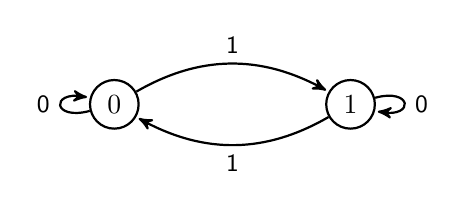
\begin{tikzpicture}[->,>=stealth',shorten >=1pt,auto,node distance=3cm, thick,main node/.style={circle,draw}]
      \node[main node] (R) {1};
      \node[main node] (L) [left of=R] {0};
      \path[every node/.style={font=\sffamily\small}]
      (L) edge [loop left] node {0} (L)
          edge [bend left] node {1} (R)
      (R) edge [loop right] node {0} (R)
          edge [bend left] node {1} (L);
  \end{tikzpicture}
  \end{center}
  More generally, a $C$-state DFA can be represented as a labeled graph of $C$ nodes. The set $\mathcal{S}$ of states on which the automaton will output $1$ at the end of the computation is known as the set of \textbf{accepting states}. We formally summarize it below. 

  \begin{definition}
  A \textbf{deterministic finite automaton (DFA)} with $C$ states over $\{0, 1\}$ is a pair $(T, \mathcal{S})$ with
  \[T: [C] \times \{0,1\} \longrightarrow [C]\]
  and $\mathcal{S} \subset [C]$. The finite function $T$ is known as the \textbf{transition function} of the DFA. The set $\mathcal{S}$ is known as the set of \textbf{accepting states}. 

  Let $F: \{0,1\}^* \longrightarrow \{0,1\}$ be a Boolean function with the infinite domain $\{0,1\}^*$. We say that $(T, \mathcal{S})$ \textbf{computes} a function $F: \{0,1\}^* \longrightarrow \{0,1\}$ if for every $n \in \mathbb{N}$ and $x \in \{0,1\}^n$, if we define $s_0 = 0$ and $s_{i+1} = T(s_i, x_i)$ for every $i \in [n]$, then 
  \[s_n \in \mathcal{S} \iff F(x) = 1\]
  \end{definition}

  Note that the transition function $T$ is a finite function specifying the table of "rules" for which the graph evolves. By defining the DFA $C$ with $(T, \mathcal{S})$, we have essentially reduced a specific type of infinite Boolean function (a single-pass constant-memory algorithm) into a graph and a finite transition function. 

  When constructing a deterministic finite automaton, it helps to start by thinking of it as a single-pass constant-memory algorithm, and then translate this program into a DFA. 

  \begin{definition}
  We say that a function $F: \{0,1\}^* \longrightarrow \{0,1\}$ is \textbf{DFA computable} if there exists some DFA that computes $F$. 
  \end{definition}

  \begin{theorem}
  Let $DFACOMP$ be the set of all Boolean functions $F: \{0,1\}^* \longrightarrow \{0,1\}$ such that there exists a DFA computing $F$. Then, $DFACOMP$ is countable. 
  \end{theorem}

  \begin{lemma}
  The set of all Boolean functions $\{f\;|\; f: \mathbb{N} \longrightarrow \{0,1\}\}$ are uncountable. 
  \end{lemma}

  \begin{corollary}[Existence of DFA-uncomputable functions]
  There exists a Boolean function $F: \{0,1\}^* \longrightarrow \{0,1\}$ that is not computable by \textit{any} DFA. 
  \end{corollary}

  \subsection{Regular Expressions}
  Searching for a piece of text is a common task in computing. At its heart, the \textit{search problem} is quite simple. We have a collection $X = \{x_0, ..., x_k\}$ of strings (e.g. files on a hard-drive, or student records in a database), and the user wants to find out the subset of all the $x \in X$ that are \textit{matched} by some pattern. In full generality, we can allow the user to specify the pattern by specifying a (computable) function $F: \{0,1\}^* \longrightarrow \{0,1\}$, where $F(x) = 1$ corresponds to the pattern matching $x$. That is, the user provides a program $P$ and the system returns all $x \in X$ such that $P(x) = 1$. 

  However, we don’t want our system to get into an infinite loop just trying to evaluate the program $P$. For this reason, typical systems for searching files or databases do not allow users to specify the patterns using full-fledged programming languages. Rather, such systems use restricted computational models that on the one hand are rich enough to capture many of the queries needed in practice, but on the other hand are restricted enough so that queries can be evaluated very efficiently on huge files and in particular cannot result in an infinite loop. One of the most popular such computational models is \textit{regular expressions}. 

  \begin{definition}
  A \textbf{regular expression $e$} over an alphabet $\Sigma$ is a string over $\Sigma \cup \{(, ), |, *, \emptyset, ""\}$ that has one of the following forms: 
  \begin{enumerate}
      \item $e = \sigma$ where $\sigma \in \Sigma$ 
      \item $e = (e^\prime \,|\, e^{\prime\prime})$ where $e^\prime, e^{\prime\prime}$ are regular expressions
      \item $e = (e^\prime)(e^{\prime\prime})$ where $e^\prime, e^{\prime\prime}$ are regular expressions. The parentheses are often dropped, so this is written $e^\prime \, e^{\prime\prime}$
      \item $e = (e^\prime)^*$ where $e^\prime$ is a regular expression
  \end{enumerate}
  Finally, we also allow the following "edge cases": $e = \emptyset$ and $e = ""$. These are the regular expressions corresponding to accepting no strings and accepting only the empty string, respectively. 
  \end{definition}

  \begin{example}
  The following are regular expressions over the alphabet $\{0,1\}$. 
  \[\big( 00(0^*)|11(1^*)\big)^* \;\;\;\;\; 00^*|11\]
  \end{example}

  Every regular expression $e$ corresponds to a function $\Phi_e : \Sigma^* \longrightarrow \{0,1\}$ where $\Phi_e (x) = 1$ if $x$ \textit{matches} the regular expression. The definition is tedious. 

  \begin{definition}
  Let $e$ be a regular expression over the alphabet $\Sigma$. The function $\Phi_e : \Sigma^* \longrightarrow \{0,1\}$ is defined as follows: 
  \begin{enumerate}
      \item If $e = \sigma$, then $\Phi_e (x) = 1$ iff $x = \sigma$ 
      \item If $e = (e^\prime \,|\, e^{\prime\prime})$, then $\Phi_e (x) = \Phi_{e^\prime} (x) \vee \Phi_{e^{\prime\prime}} (x)$ where $\vee$ is the OR operator. 
      \item If $e = (e^\prime) (e^{\prime\prime})$, then $\Phi_e (x) = 1$ iff there is some $x^\prime, x^{\prime\prime} \in \Sigma^*$ such that $x$ is the concatenation of $x^\prime$ and $x^{\prime\prime}$ and $\Phi_{e^\prime} (x^\prime) = \Phi^{e^{\prime\prime}} (x^{\prime\prime}) = 1$ 
      \item If $e = (e^\prime)^*$ then $\Phi_e (x) = 1$ iff there is some $k \in \mathbb{N}$ and some $x_0, x_1, ..., x_{k-1} \in \Sigma^*$ such that $x$ is the concatenation $x_0, x_1, ..., x_{k-1}$ and $\Phi_{e^\prime} (x_i) = 1$ for every $i \in [k]$. 
      \item For the edge cases, $\Phi_{\emptyset}$ is the $0$ function, and $\Phi_{""}$ is the function that only outputs $1$ on the empty string $""$. 
  \end{enumerate}
  It is said that a regular expression $e$ over $\Sigma$ \textbf{matches} a string $x \in \Sigma^*$ if $\Phi_e (x) = 1$. 
  \end{definition}

  A Boolean function is called \textit{regular} if it outputs 1 on precisely the set of strings that are matched by some regular expression. 

  \begin{definition}
  Let $\Sigma$ be a finite set and $F: \Sigma^* \longrightarrow \{0,1\}$ be a Boolean function. We say that $F$ is \textbf{regular} if $F = \Phi_e$ for some regular expression $e$. 

  Similarly, for every formal language $L \subset \Sigma^*$, we say that $L$ is regular if and only if there is a regular expression $e$ such that $x \in L$ iff $e$ matches $x$. 
  \end{definition}

  \begin{definition}
  The set of functions computable by DFAs is the same as the set of languages that can be recognized by regular expressions. 
  \end{definition}

\section{Turing Machines}

  Similar to how a person does calculations by reading from and writing to a single cell of a paper at a time, a Turing machine is a hypothetical machine that reads from its "work tape" a single symbol from a finite alphabet $\Sigma$ and uses that to update its state, write to tape, and possibly move to an adjacent cell. To compute a function $F$ using this machine, we initialize the tape with the input $x \in \{0,1\}^*$ and our goal is to ensure that the tape will contain the value $F(x)$ at the end of the computation. Specifically, a computation of a Turing machine $M$ with $k$ states and alphabet $\Sigma$ on input $x \in \{0,1\}^*$ is formally defined as follows. 

  \begin{definition}[Turing Machine]
  A (one tape) \textbf{Turing machine} with $k$ states and alphabet $\Sigma \supset \{0, 1, \triangleright, \emptyset\}$ is represented by a \textbf{transition function} 
  \[\delta_M: [k] \times \Sigma \longrightarrow [k] \times \Sigma \times \{\mathsf{L, R, S, H}\}\]
  For every $x \in \{0,1\}^*$, the \textit{output} of $M$ on input $x$, denoted by $M(x)$, is the result of the following process: 
  \begin{enumerate}
      \item We initialize $T$ to be the infinite sequence (also represented by a tape)
      \[\triangleright, x_0, x_1, ..., x_{n-1}, \emptyset, \emptyset, ...\]
      where $n = |x|$. That is, $T[0] = \triangleright, T[i+1] = x_i$ for $i \in [n]$, and $T[i] = \emptyset$ for $i>n$.)
      \item We also initialize $i = 0$ (the head is at the starting position) and we begin with the initial state $s=0$, $s \in [k]$. 
      \item We then repeat the following process which is defined according to the transition function: 
      \begin{enumerate}
          \item Let $(s^\prime, \sigma^\prime, D) = \delta_M (s, T[i])$.
          \item Set $s \rightarrow s^\prime$, $T[i] \rightarrow \sigma^\prime$
          \item If $D = \mathsf{R}$, then set $i \rightarrow i+1$, if $D = \mathsf{L}$, then set $i \rightarrow \max\{i-1,0\}$. If $D = \mathsf{S}$, then we keep $i$ the same. 
          \item If $D = \mathsf{H}$, then halt. 
      \end{enumerate}
      Colloquially, at each step, the machine reads the symbol $\sigma \in T[i]$ that is in the $i$th location of the tape. Bsaed on this symbol and its state $s$, the machine decides on
      \begin{enumerate}
          \item What symbol $\sigma^\prime$ to write on the tape
          \item Whether to move $\mathsf{L}$eft ($i \rightarrow i-1)$, $\mathsf{R}$ight ($i \rightarrow i+1$), $\mathsf{S}$tay in place, or $\mathsf{H}$alt the computation 
          \item What is going to be the new state $s \in [k]$
      \end{enumerate}
      \item If the process above halts, then $M$'s output, denoted by $M(x)$ is the string $y \in \{0,1\}^*$ obtained by concatenating all the symbols in $\{0,1\}$ in positions $T[0], ..., T[i]$ where $i+1$ is the first location in the tape containing $\emptyset$. 
      \item If the Turing machine does not halt then we denote $M(x) = \perp$. 
  \end{enumerate}
  \end{definition}

  We can visualize a Turing machine as a table and a tape labeled below.
  \begin{center}
  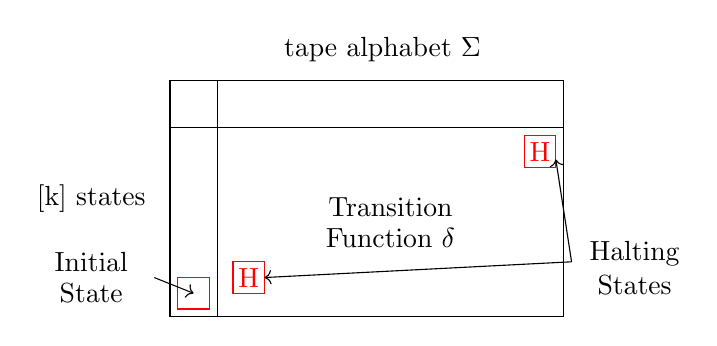
\begin{tikzpicture}
      \draw (-2,-2) rectangle (3,1);
      \draw (-1.4,-2)--(-1.4,1);
      \draw (-2,0.4)--(3,0.4);
      \node (k) at (-3, -0.5) {[k] states};
      \node (a) at (0.7, 1.4) {tape alphabet $\Sigma$};
      \node (q) at (0.8, -0.6) {Transition};
      \node (p) at (0.8, -1) {Function $\delta$};
      \node (i) at (-3, -1.3) {Initial};
      \node (i) at (-3, -1.7) {State};
      \draw[red] (-1.9,-1.9) rectangle (-1.5,-1.5);
      \draw[->] (-2.2,-1.5)--(-1.7,-1.7);
      \draw[red] (-1.2,-1.7) rectangle (-0.8,-1.3);
      \draw[red] (2.9,0.3) rectangle (2.5,-0.1);
      \node (h) at (3.9, -1.2) {Halting};
      \node (h) at (3.9, -1.6) {States};
      \draw[->] (3.1, -1.3)--(2.9, 0);
      \draw[->] (3.1, -1.3) --(-0.8,-1.5);
      \node[red] at (2.7,0.1) {H};
      \node[red] at (-1,-1.5) {H};
  \end{tikzpicture}
  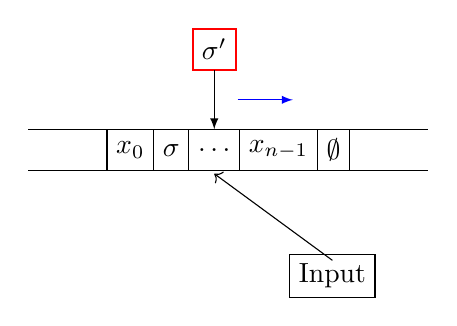
\begin{tikzpicture}[every node/.style={block},
          block/.style={minimum height=1.5em,outer sep=0pt,draw,rectangle,node distance=0pt}]
     \node (A) {$\ldots$};
     \node (B) [left=of A] {$\sigma$};
     \node (C) [left=of B] {$x_0$};
     \node (D) [right=of A] {$x_{n-1}$};
     \node (E) [right=of D] {$\emptyset$};
     \node (F) [above = 0.75cm of A,draw=red,thick] {$\sigma^\prime$};
     \draw[-latex] (F) -- (A);
     \draw[-latex,blue] ($(F.east)!0.5!(A.east)$) -- ++(7mm,0);
     \draw (C.north west) -- ++(-1cm,0) (C.south west) -- ++ (-1cm,0) 
                   (E.north east) -- ++(1cm,0) (E.south east) -- ++ (1cm,0);
      \draw[->] (1.5,-1.4)--(0,-0.3);
      \node[style={}] (i) at (1.5, -1.6) {Input};
  \end{tikzpicture}
  \end{center}

  In fact, all modern computing devices are Turing machines at heart. You input a string of bits, the machine flips a bunch of switches, and outputs another string of bits. 

  \begin{example}[Turning Machine for Palindromes]
  Let $PAL$ be the function that on input $x \in \{0,1\}^*$, outputs 1 if and only if $x$ is an (even length) \textit{palindrome}, in the sense that
  \[x = w_0 ... w_{n-1} w_{n-1} w_{n-2} ... w_0\]
  for some $n \in \mathbb{N}$ and $w \in \{0,1\}^*$. We will now describe a Turing machine that computes $PAL$. To specify $M$, we need to specify
  \begin{enumerate}
      \item $M$'s tape alphabet $\Sigma$ which should contain at least the symbols 0, 1, $\triangleright$, and $\emptyset$, and
      \item $M$'s transition function which determines what action $M$ takes when it reads a given symbol while it is in a particular state. 
  \end{enumerate}
  For this specific Turing machine, we will use the alphabet $\{0,1,\triangleright, \emptyset, \times\}$ and will have $k=13$ states, with the following labels for the numbers. 
  \begin{center}
  \begin{tabular}{l|l|l|l}
      State & Label & State & Label\\
      \hline
      0 & $\texttt{START}$ & 7&$\texttt{ACCEPT}$\\
      1& $\texttt{RIGHT\_0}$ & 8&$\texttt{OUTPUT\_0}$\\
      2&$\texttt{RIGHT\_1}$ & 9&$\texttt{OUTPUT\_1}$ \\
      3&$\texttt{LOOK\_FOR\_0}$ & 10&$\texttt{0\_AND\_BLANK}$\\
      4&$\texttt{LOOK\_FOR\_1}$ & 11&$\texttt{1\_AND\_BLANK}$\\
      5&$\texttt{RETURN}$ & 12&$\texttt{BLANK\_AND\_STOP}$\\
      6&$\texttt{REJECT}$ & & \\
  \end{tabular}
  \end{center}
  The operation of our Turning machine, in words, is as such: 
  \begin{enumerate}
      \item $M$ starts in the state $\texttt{START}$ and goes right, looking for the first symbol that is 0 or 1. If it finds $\emptyset$ before it hits such a symbol then it moves to the $\texttt{OUTPUT\_1}$ state. 
      \item Once $M$ finds such a symbol $b \in \{0,1\}$, $M$ deletes $b$ from the tape by writing the $\times$ symbol, it enters either the $\texttt{RIGHT\_0}$ or $\texttt{RIGHT\_1}$ mode according to the value of $b$ and starts moving rightwards until it hits the first $\emptyset$ or $\times$ symbol. 
      \item Once $M$ finds this symbol, it goes into the state $\texttt{LOOK\_FOR\_0}$ or $\texttt{LOOK\_FOR\_1}$ depending on whether it was in the state $\texttt{RIGHT\_0}$ or $\texttt{RIGHT\_1}$ and makes one left move. 
      \item In the state $\texttt{LOOK\_FOR\_}b$, $M$ checks whether the value on the tape is $b$. If it is, then $M$ deletes it by changing its value to $\times$, and moves to the state $\texttt{RETURN}$. Otherwise, it changes to the $\texttt{OUTPUT\_0}$ state. 
      \item The $\texttt{RETURN}$ state means that $M$ goes back to the beginning. Specifically, $M$ moves leftward until it hits the first symbol that is not $0$ or $1$, in which case it changes its state to $\texttt{START}$. 
      \item The $\texttt{OUTPUT\_}b$ states mean that $M$ will eventually output the value $b$. In both the $\texttt{OUTPUT\_0}$ and $\texttt{OUTPUT\_1}$ states, $M$ goes left until it hits $\triangleright$. Once it doe sso, it makes a right step and changes to the $\texttt{1\_AND\_BLANK}$ or $\texttt{0\_AND\_BLANK}$ state respectively. In the latter states, $M$ writes the corresponding value, moves right and changes to the $\texttt{BLANK\_AND\_STOP}$ state, in which it writes $\emptyset$ to the tape and halts. 
  \end{enumerate}
  The above description can be turned into a table describing for each one of the $13 \cdot 5 = 65$ combinations of state and symbol, what the Turing machine will do when it is in that state and it reads that symbol. This table is the \textit{transition function} of the Turing machine. 
  \end{example}

  \begin{definition}[Computable Functions]
  Let $F: \{0,1\}^* \longrightarrow \{0,1\}^*$ be a (total) function and let $M$ be a Turing machine. We say that $M$ \textbf{computes} $F$ if for every $x \in \{0,1\}^*$, $M(x) = F(x)$. We say that a function $F$ is \textbf{computable} if there exists a Turing machines $M$ that computes it. 
  \end{definition}

  It turns out that being computable in the sense of a Turing machine is equivalent to being computable in virtually any reasonable model of computation. This statement is known as the \textbf{Church-Turing Thesis}. Therefore, this definition allows us to precisely define what it means for a function to be computable by \textit{any possible algorithm}. 

  \begin{definition}[The class \textbf{R}]
  We define $\textbf{R}$ to be the set of all computable functions $F: \{0,1\}^* \longrightarrow \{0,1\}$. 
  \end{definition}

  \subsection{NAND-TM Programs}
  In addition to having a physical interpretation, Turing machines can also be interpreted as programs. 
  \begin{enumerate}
      \item The \textit{tape} becomes a \textit{list} or \textit{array} that can hold values from the finite set $\Sigma$. 
      \item The \textit{head position} can be thought of as an integer-valued variable that holds integers of unbounded size. 
      \item The \textit{state} is a \textit{local register} that can hold one of a fixed number of values in $[k]$. 
  \end{enumerate}
  In general, every Turing machine $M$ is equivalent to a program similar to the following: 
  \begin{lstlisting}
  #Gets an array Tape initialized to [">", x_0,..., x_(n-1), " ", " ", ...]
  def M(Tape): 
      state = 0
      i     = 0  #holds head location
      while(True): 
          #Move head, modify state, write to tape based on current state and 
          #cell at head below are just examples for how program looks 
          #for a particular transition function
          if Tape[i]=="0" and state==7: #T_M(7,"0")=(19,"1","R") 
              i += 1
              Tape[i]="1"
              state = 19
          elif Tape[i]==">" and state == 13: #T_M(13,">")=(15,"0","S")
              Tape[i] ="0"
              state = 15
          elif... 
              ...
          elif Tape[i]==">" and state == 29: #T_M(29,">")=(.,.,"H")
              break  #Halt
  \end{lstlisting}
  If we were using Boolean variables, then we can encode the $\texttt{state}$ variables using $\left\lceil{\log k}\right\rceil$ bits. 

  Note that in the code above, two new concepts are introduced: 
  \begin{enumerate}
      \item \textit{Loops}: NAND-CIRC is a straight line programming language. That is, a NAND-CIRC program of $s$ lines takes exactly $s$ steps of computation and hence in particular, cannot even touch more than $3s$ variables. \textit{Loops} allow us to use a fixed-length program to encode the instructions for a computation that can take an arbitrary amount of time. 
      \item \textit{Arrays}: A NAND-CIRC program of $s$ lines touches at most $3s$ variables. While we can use variables with names such as $\texttt{Foo\_17}$ or $\texttt{Bar[22]}$ in NAND-CIRC, they are not true arrays, since the number in the identifier is a constant that is not "hardwired" into the program. NAND-TM contains actual arrays that can have a length that is not a priori bounded. 
  \end{enumerate}
  The following equation summarizes the concepts: 
  \[\text{NAND-TM} = \text{NAND-CIRC} + \text{loops} + \text{arrays}\]
  Surprisingly, adding loops and arrays to NAND-CIRC is enough to capture the full power of all programming languages. Hence, we could replace NAND-TM with any of Python, C, Javascript, etc. 

  Concretely, the NAND-TM programming language adds the following features on top of NAND-CIRC: 
  \begin{enumerate}
      \item We add a special \textit{integer valued variable} $i$. All other variables in NAND-TM are Boolean valued (as in NAND-CIRC). 
      \item Apart from $i$, NAND-TM has two kinds of varibales: \textit{scalars} and \textit{arrays}. \textit{Scalar} variables hold one bit (just as in NAND-CIRC). \textit{Array} variables hold an unbounded number of bits. At any point in the computation we can access the array variables at the location indexed by $\texttt{i}$ using $\texttt{Foo[i]}$. We cannot access the arrays at loctions other than the one pointed by $\texttt{i}$. 
      \item We use the convention that \textit{arrays} always start with a capital letter, and \textit{scalar variables} (which are never indexed with $\texttt{i}$) start with lowercase letters. Hence, $\texttt{Foo}$ is an array and $\texttt{foo}$ is a scalar variable. 
      \item The input and output $\texttt{X}$ and $\texttt{Y}$ are not considered \textit{arrays} with values of 0s and 1s. 
      \item We add a special $\texttt{MODANDJUMP}$ instruction that takes two Boolean variables $a, b$ as input and does the following:  
      \begin{enumerate}
          \item If $a = 1, b = 1$, then $\texttt{MODANDJUMP(a, b)}$ increments $\texttt{i}$ by one and jumps to the first line of the program. 
          \item If $a = 0, b = 1$, then $\texttt{MODANDJUMP}(a, b)$ decrements $\texttt{i}$ by one and jumps to the first line of the program. If $\texttt{i}$ already equals 0, then it stays at 0.
          \item If $a = 1, b = 0$, then $\texttt{MODANDJUMP}(a, b)$ jumps to the first line of the program without modifying $\texttt{i}$. 
          \item If $a = b = 0$, then $\texttt{MODANDJUMP}(a, b)$ halts execution of the program.
      \end{enumerate}
      \item The $\texttt{MODANDJUMP}$ instruction always appears in the last line of a NAND-TM program and nowhere else. 
      \item Turing machines have the special symbol $\emptyset$ to indicate that tape location is "blank" or "uninitialized." In NAND-TM there is no such symbol, and all variables are \textit{Boolean}, containing either $0$ or $1$. All variables and locations either default to $0$ if they have not been initialized to another value. To keep track of whether a $0$ in an array corresponds to a true 0 or to an uninitialized cell, a programmer can always add to an array $\texttt{Foo}$ a \textit{companion array} $\texttt{Foo\_nonblank}$ and set $\texttt{Foo\_nonblank[i]}$ to $1$ whenever the $\texttt{i}$th location is initialized. In particular, we will use this convention for the input and output arrays $\texttt{X}$ and $\texttt{Y}$. Therefore, a NAND-TM program has \textit{four} special arrays $\texttt{X, X\_nonblank, Y, Y\_nonblank}$. 
  \end{enumerate}
  Therefore, when a NAND-TM program is executed on input $x \in \{0,1\}^*$ of length $n$, the first $n$ cells of $\texttt{X}$ are initialized to $x_0, ..., x_{n-1}$ and the first $n$ cells of $\texttt{X\_noblank}$ are initalized to $1$ (all uninitialized cells default to $0$). The output of a NAND-TM program is the string $\texttt{Y[0], ..., Y[m-1]}$ where $m$ is the smallest integer such that $\texttt{Y\_nonblank[m]} = 0$. 

  We now formally define a NAND-TM program. 

  \begin{definition}[NAND-TM Programs]
  A \textbf{NAND-TM program} consists of a sequence of lines of the form $\texttt{foo = NAND(bar, blah)}$ and ending with a line of the form $\texttt{MODANDJMP(foo, bar)}$, where $\texttt{foo, bar, blah}$ are either \textit{scalar variables} (sequence of letters, digits, and underscores) or \textit{array variables} of the form $\texttt{Foo[i]}$ (starting with capital letters and indexed by $\texttt{i}$). The program has the array variables $\texttt{X, X\_nonblank}$, $\texttt{Y, Y\_nonblank}$ and the index variables $\texttt{i}$ built in, and can use additional array and scalar variables. 

  If $P$ is a NAND-TM program and $x \in \{0,1\}^*$ is an input then an execution of $P$ on $x$ is the following process: 
  \begin{enumerate}
      \item The arrays $\texttt{X}$ and $\texttt{X\_nonblank}$ are initialized by $\texttt{X[i]} = x_i$ and $\texttt{X\_nonblank[i]} = 1$ for all $i \in [|x|]$. All other variables and cells are initialized to $0$. The index variable $\texttt{i}$ is also initialized to $0$. 
      \item The program is executed line by line. When the last line $\texttt{MODANDJMP(foo, bar)}$ is executed we do as follows: 
      \begin{enumerate}
          \item If $\texttt{foo, bar} = 1, 0$, jump to the first line without modifying the value of $\texttt{i}$. 
          \item If $\texttt{foo, bar} = 1, 1$, incremenet $\texttt{i}$ by one and jump to the first line. 
          \item If $\texttt{foo, bar} = 0, 1 $, then decrement $\texttt{i}$ by one (unless it is already 0) and jump to the first line. 
          \item If $\texttt{foo, bar} = 0, 0$, halt and output $\texttt{Y[0], ..., Y[m-1]}$ where $m$ is the smallest integer such that $\texttt{Y\_nonblank[m]} = 0$. 
      \end{enumerate}
  \end{enumerate}
  \end{definition}

  Here are some components of Turing machines and their analogs in NAND-TM programs. 
  \begin{enumerate}
      \item The \textit{state} of a Turing machine is equivalent to the \textit{scalar-variables} such as $\texttt{foo, bar, etc.}$, each taking values in $\{0,1\}$. 
      \item The \textit{tape} of a Turing machines is equivalent to the \textit{arrays}, where the component of each array is either $0$ or $1$. 
      \item The \textit{head location} is equivalent to the \textit{index variable}
      \item \textit{Accessing memory}: At every step the Turing machine has access to its local state, but can only access the tape at the position of the current head location. In a NAND-TM program, it has access to all the scalar variables, but can only access the arrays at the location $\texttt{i}$ of the index variable. 
      \item A Turing machine can move the head location by at most one position in each step, while a NAND-TM program can modify the index $\texttt{i}$ by at most one. 
  \end{enumerate}

  \begin{theorem}[Equivalence of Turing Machines and NAND-TM programs]
  For every function $F: \{0,1\}^* \longrightarrow \{0,1\}^*$, $F$ is computable by a NAND-TM program $P$ if and only if there is a Turing machine $M$ that computes $F$. 
  \end{theorem}

  \begin{center}
  \begin{tabular}{l|l|l}
      Setting & Specification & Implentation \\
      \hline
      Finite Computation& $F: \{0,1\}^n \rightarrow \{0,1\}^m$ & Circuit, Straightline program \\
      Infinite Computation & $F: \{0,1\}^* \rightarrow \{0,1\}^*$ & Algorithm, Turing Machine, Program
  \end{tabular}
  \end{center}

  Finally, we can use syntactic sugar to make NAND-TM programs easier to write. For starters, we can use all of the syntactic sugar of NAND-CIRC, such as macro definitions and conditionals (if/then). However, we can go beyond this and achieve: 
  \begin{enumerate}
      \item Inner loops such as the $\texttt{while}$ and $\texttt{for}$ operations common to many programming languages. 
      \item Multiple index variables (e.g. not just $\texttt{i}$ but also $\texttt{j, k}$, etc.). 
      \item Arrays with more than one dimension (e.g., $\texttt{Foo[i][j]}$). 
  \end{enumerate}
  This means that the set of functions computable by NAND-TM with this feature is the same as the set of functions computable by standard NAND-TM.

  \subsubsection{Uniformity of Computation}
  \begin{definition}
  The notion of a single algorithm that can compute functions of all input length is known as \textbf{uniformity} of computation. 
  \end{definition}

  Hence we think of Turing machines and NAND-TM as \textit{uniform} models of computation, as opposed to Boolean circuits of NAND-CIRC, which are non-uniform models, in which we have to specify a different program for every input length. This uniformity leads to another crucial difference between Turing machines and circuits. Turing machines can have inputs and outputs that are longer than the description of the machine as a string, and in particular there exists a Turing machine that can "self replicate" in the sense that it can print its own code. This is extremely useful. 

  In summary, the main differences between uniform and non-uniform models are described as such: 
  \begin{enumerate}
      \item \textbf{Non-uniform computational models}: Examples are NAND-CIRC programs and Boolean circuits. These are models where each individual program/circuit can compute a \textit{finite} function 
      \[f: \{0,1\}^n \longrightarrow \{0,1\}^m\]
      We have seen that \textit{every} finite function can be computed by \textit{some} program/circuit. To discuss computation of an \textit{infinite} function $F: \{0,1\}^* \longrightarrow \{0,1\}^*$, we need to allow a \textit{sequence} $\big\{ P_n \big\}_{n \in \mathbb{N}}$ of programs/circuits (one for every input length), but this does not capture the notion of a \textit{single algorithm} to compute the function $F$. 
      \item \textbf{Uniform computational models}: Examples are Turing machines and NAND-TM programs. These are models where a single program/Turing machine can take inputs of \textit{arbitrary length} and hence compute an \textit{infinite} function 
      \[F: \{0,1\}^* \longrightarrow \{0,1\}^* \]
      The number of steps that a program/machine takes on some input is not a priori bounded in advance and in particular there is a chance that it will enter into an \textit{infinite loop}. Unlike the non-uniform case, we have \textit{not} shown that every infinite function can be computed by some NAND-TM program/Turing machine. 
  \end{enumerate}

  \subsection{RAM Machines and NAND-RAM Programs}
  Note that since Turing machines (and NAND-TM programs) can only access one locations of arrays/tape at a time, they do not have \textit{RAM}.

  \begin{definition}
  The computational model that models access to such a memory is the \textbf{RAM machine}. The \textbf{memory} of a RAM machine is an array of unbounded size where each cell can store a single \textbf{word}, which can be thought of as a string in $\{0,1\}^\omega$ and also (equivalently) as a number in $[2^\omega]$. 
  \end{definition}

  For example, many modern computing architectures use 64-bit words, in which every memory location holds a string in $\{0,1\}^{64}$. The parameter $\omega$ is known as the \textit{word size}. In addition to the memory array, a RAM machine also contains a constant number of \textbf{registers} $r_0, r_1, ..., r_{k-1}$, each of which can also contain a word. 

  The oeprations a RAM machine can carry out include: 
  \begin{enumerate}
      \item \textbf{Data movement}: Load data from a certain cell in memory into a register or store the contents of a register into a certain cell of memory. A RAM machine can directly access any cell of memory without having to move the “head” (as Turing machines do) to that location. That is, in one step a RAM machine can load into register $r_i$ the contents of the memory cell indexed by register $r_j$, or store into the memory cell indexed by register $r_j$ the contents of register $r_i$. 
      \item \textbf{Computation}: RAM machines can carry out computation on registers such as arithmetic operations, logical operations, and comparisons. 
      \item \textbf{Control flow}: As in the case of Turing machines, the chose of what instruction to perform next can depend on the state of the RAM machine, which is captured by the contents of its register. 
  \end{enumerate}

  Just as the NAND-TM programming language models Turing machines, we can also define a \textbf{NAND-RAM programming language} that models RAM machines. The NAND-RAM programming language extends NAND-TM by adding the following features: 
  \begin{enumerate}
      \item The variables of NAND-RAM are allowed to be (non-negative) \textit{integer valued} rather than only Boolean. That is, a scalar variable $\texttt{foo}$ holds a nonnegative integer in $\mathbb{N}$ and an array variable $\texttt{Bar}$ holds an array of integers. As in the case of RAM machines, we will not allow integers of unbounded size. 
      \item We allow \textit{indexed access} to arrays. If $\texttt{foo}$ is a scalar and $\texttt{Bar}$ is an array, then $\texttt{Bar[foo]}$ refers to the location of $\texttt{Bar}$ indexed by the value of $\texttt{foo}$. Note that this means that we don't need to have a special index variable $\texttt{i}$ anymore. 
      \item We will assume that for Boolean operations such as $\texttt{NAND}$, a zero valued integer is considered as \textit{false}, and a nonzero valued integer is considered as \textit{true}. 
      \item In addition to $\texttt{NAND}$, NAND-RAM also includes all the basic arithmetic operations of addition, subtraction, multiplication, integer division, as well as comparisions (equal, greater/less than, etc.). 
      \item NAND-RAM includes conditional statements $\texttt{if/then}$ as a part of the language. 
      \item NAND-RAM contains looping constructs such as $\texttt{while}$ and $\texttt{do}$ as part of the language. 
  \end{enumerate}

  It is easy to see that NAND-RAM programs are clearly more powerful than NAND-TM, and so if a function $F$ is computable by a NAND-TM program then it can be computed by a NAND-RAM program. It turns out to be true that if a function is computable by a NAND-RAM program, then it can also be computed by a NAND-TM program. 

  \begin{theorem}
  Turing machines (aka NAND-TM programs) and RAM machines (aka NAND-RAM programs) are equivalent. That is, for every function 
  \[F: \{0,1\}^* \longrightarrow \{0,1\}^* ,\]
  $F$ is computable by a NAND-TM program if and only if $F$ is computable by a NAND-RAM program. Therefore, all four models are equivalent to one another. 
  \end{theorem}

\section{Turing Completeness and Equivalence}

  Even though the notion of computing a function using Turing machines is crucial in theory, it is not a practical way of preforming computation. But in addition to defining computable functions with Turing machines, there are many equivalent conditions of computability under a wide variety of computational models. This notion is known as \textit{Turing completeness} or \textit{Turing equivalence}. 

  Any of the standard programming languages such as C, Java, Python, Pascal, Fortran, have very similar operations to NAND-RAM. Indeed, ultimately, they can all be executed by machines which have a fixed number of registers and a large memory array. Hence, with the equivalence theorem, we can simulate any program in such a programming language by a NAND-TM program. In the other direction, it is a fairly easy programming exercise to write an interpreter for NAND-TM in any of the above programming languages. Hence we can also simulate NAND-TM programs (and Turing machines) using these programming languages. 

  \begin{definition}
  A computational system is said to be \textbf{Turing-complete} or \textbf{computationally universal} if it can be be used to simulate any Turing machine or NAND-TM. 

  Very much related, the property of being \textit{equivalent} in power to Turing machines/NAND-TM is called \textbf{Turing equivalent}. That is, two computer $P$ and $Q$ are equivalent if $P$ can simulate $Q$ and $Q$ can simulate $P$. All known Turing complete systems are Turing equivalent. 
  \end{definition}

  The equivalence between Turing machines and RAM machines allows us to choose the most convenient language for the task at hand: 
  \begin{enumerate}
      \item When we want to \textit{prove a theorem} about all programs/algorithms, we can use Turing machines (or NAND-TM) since they are simpler and easier to analyze. 
      \item If we want to show that a certain function \textit{cannot} be computed, then we will use Turing machines. 
      \item When we want to show that a function can be computed we can use RAM machines or NAND-RAM, because they are easier to program in and correspond more closely to high level programming languages we are used to. In fact, we will often describe NAND-RAM programs in an informal manner, trusting that the reader can fill in the details and translate the high level description to the precise program. (This is just like the way people typically use informal or “pseudocode” descriptions of algorithms, trusting that their audience will know to translate these descriptions to code if needed.)
  \end{enumerate}

  A formal definition of Turing completeness is as follows. This is also referred to as \textit{Godel Numbering}, which is a function that assigns to each symbol and well-formed formula of some formal language a unique natural number, called its Gödel number 

  \begin{definition}[Turing Completeness and Equivalence]
  Let $\mathcal{F}$ be the set of all partial functions from $\{0, 1\}^*$ to $\{0,1\}^*$. A \textbf{computational model} is a map
  \[\mathcal{M}: \{0,1\}^* \longrightarrow \mathcal{F}\]
  We say that a program $P \in \{0,1\}^*$ \textbf{$\mathcal{M}$-computes} a function $F \in \mathcal{F}$ if 
  \[\mathcal{M}(P) = F\]
  A computational model $\mathcal{M}$ is \textbf{Turing complete} if there is a computable map 
  \[ENCODE_{\mathcal{M}} : \{0,1\}^* \longrightarrow \{0,1\}^*\]
  such that for every Turing machine $N$ (represented as a string), $\mathcal{M}(ENCODE_\mathcal{M} (N))$ is equal to the partial function computed by $N$. 

  A computational model $\mathcal{M}$ is \textbf{Turing equivalent} if it is Turing complete and there exists a computable map $DECODE_\mathcal{M}: \{0,1\}^* \longrightarrow \{0,1\}^*$ such that for every string $P \in \{0,1\}^*$, $N = DECODE_\mathcal{M} (P)$ is a string representation of a Turing machine that computes the function $\mathcal{M}(P)$. 
  \end{definition} 

  \subsection{Cellular Automata}
  Many physical systems can be described as consisting of a large number of elementary components that interact with one another. One way to model such systems is using cellular automata. This is a system that consists of a large (or even infinite) number of cells. Each cell only has a constant number of possible states. At each time step, a cell updates to a new state by applying some simple rule to the state of itself and its neighbors.

  \begin{definition}
  An example of a cellular automaton is \textbf{Conway's Game of Life}. In this automata the cells are arranged in an infinite two dimensional grid. Each cell has only two states: 
  \begin{enumerate}
      \item Dead: which we encode as a 0
      \item Alive: which we encode as 1
  \end{enumerate}
  The next state of a cell depends on its previous state and the states of its 8 adjacent neighbors, which can be modeled with a transition function
  \[r: \Sigma^8 \longrightarrow \Sigma\]
  A dead cell becomes alive only if exactly three of its neighbors are alive. A live cell continues to live if it has two or three live neighbors. 
  \end{definition}

  Even though the number of cells is potentially infinite, we can encode the state using a finite-length string by only keeping track of the live cells. If we initialize the system in a configuration with a finite number of live cells, then the number of live cells will stay finite in all future steps. Note that this is a discrete time Markov chain. 

  Since the cells in the game of life are arranged in an infinite two-dimensional grid, it is an example of a \textit{two dimensional cellular automaton}. We can get even simpler by setting a \textit{one dimensional cellular automaton}, where the cells are arranged in an infinite line. 

  \begin{theorem}
  Conway's Game of Life is Turing complete. 
  \end{theorem}

  \subsubsection{One-Dimensional Cellular Automata}
  \begin{definition}
  Let $\Sigma = \{0, 1, \emptyset\}$. A \textbf{one-dimensional cellular automaton} of alphabet $\Sigma$ is described by a \textit{transition rule}
  \[r: \Sigma^3 \longrightarrow \Sigma\]
  A \textbf{configuration} of the automaton $r$ is a function $A: \mathbb{Z} \longrightarrow \Sigma$; that is, $A$ just represents an infinite sequence of letters in the alphabet $\Sigma$. If an automaton with rule $r$ is in configuration $A$, then its next configuration $A^\prime = NEXT_r (A)$, is the function $A^\prime$ such that 
  \[A^\prime (i) = r\big( A(i-1), A(i), A(i+1)\big)\]
  In other words, the next state of the automaton $r$ at point $i$ is obtained by applying the rule $r$ to the values of $A$ at $i$ and its two neighbors. 

  It is also said that a configuration of an automaton $r$ is \textbf{finite} if there is only some finite number of indices $i_0, ..., i_{j-1}$ in $\mathbb{Z}$ such that $A(i_j) \neq \emptyset$. 
  \end{definition}

  If the alphabet is only $\{0, 1\}$, then there can be a total of $2^8 = 256$ total possible one dimensional cellular automata. For example, the cellular automaton with the transition rule
  \[r(L, C, R) \equiv C + R + CR + LCR \pmod{2}\]
  can be expressed with the table (called rule 110)

  \begin{center}
  \begin{tabular}{c|c|c|c|c|c|c|c}
      111	&110	&101	&100	&011	&010	&001	&000 \\
      \hline
      0&1&1&0&1&1&1&0
  \end{tabular}
  \end{center}

  However, many of them are trivially equivalent to each other up to a simple transformation of the underlying geometry, such as with reflections, translations, or rotations. This reduces the possible unique automata to 88, only one of which is Turing complete. 

  \begin{theorem}
  The Rule 110 cellular automaton is Turing complete. That is, any calculation or computer program can be simulated using this automaton. 
  \end{theorem}

  \begin{definition}[Configuration of Turing Machines]
  Let $M$ be a Turing machine with tape alphabet $\Sigma$ and state space $[k]$. A \textbf{configuration} of $M$ is a string 
  \[\alpha \in \overline{\Sigma}^*, \text{ where } \overline{\Sigma} = \Sigma \times \big( \{ \cdot \} \cup [k] \big)\]
  that satisfies that there is exactly one coordinate $i$ for which $\alpha_i = (\sigma, s)$ for some $\sigma \in \Sigma$ and $s \in [k]$. For all other coordinates $j$, $\alpha_j = (\sigma^\prime, \cdot)$ for some $\sigma^\prime \in \Sigma$. A configuration of $\alpha \in \overline{\Sigma}^*$ of $M$ corresponds to the following staet of its execution: 
  \begin{enumerate}
      \item $M$'s tape contains $\alpha_{j, 0}$ for all $j < |\alpha|$ and contains $\emptyset$ for all positions that are at least $|\alpha|$, where we let $\alpha_{j, 0}$ be the value $\sigma$ such that $\alpha_j = (\sigma, t)$ with $\sigma \in \Sigma$ and $t \in \{\cdot\} \cup [k]$. In other words, since $\alpha_j$ is a pair of an alphebet symbol $\sigma$ and either a state in $[k]$ or the symbol $\cdot$, $\alpha_{j, 0}$ is the first component $\sigma$ of this pair. 
      \item $M$'s head is in the unique position $i$ for which $\alpha_i$ has the form $(\sigma, s)$ for $s \in [k]$, and $M$'s state is equal to $s$. 
  \end{enumerate}
  Informally, a configuration can be interpreted simply as a string that encodes a \textit{snapshot} of the Turing machine at a given point in the execution. It is also called a \textit{core dump}. Such a snapshot must encode the following components: 
  \begin{enumerate}
      \item The current head position. 
      \item The full contents of the large scale memory, that is the tape. 
      \item The contents of the "local registers," that is the state of the machine. 
  \end{enumerate}
  \end{definition}

  \subsection{Lambda Calculus}
  The \textbf{Lambda calculus} is an abstract mathematical theory of computation, involving $\lambda$ functions. It is a Turing complete language. $\lambda$ calculus allows us to define "anonymous" functions. For example, instead of giving a name $f$ to a function and defining it as 
  \[f(x) = x^2\]
  we can write it anonymously (without naming it at all) as 
  \[x \mapsto x^2, \text{ or equivalently, } \lambda x . x^2\]
  so $(\lambda x.x^2) (7) = 49$, or by dropping the parentheses,  $(\lambda x.x^2) 7 = 49$. That is, we can interpret $\lambda x.exp(x)$, where $exp$ is some expression as a way of specifying the anonymous function $x \mapsto exp(x)$. This notation occurs in many programming languages, such as Python, where the squaring function is written $\texttt{lambda x: x*x}$.  

  Furthermore, in $\lambda$ calculus functions are \textit{first-class objects}, meaning that we can use functions as arguments to other functions. However, \textit{all functions must take one input}. 

  \textbf{Expressions} can be thought of as programs in the language of lambda calculus. Given the notion of a variable, denoted by $x, y, z, ...$ we recursively define an expression inductively in terms of abstractions (anonymous functions) and applications as follows: 

  \begin{definition}[$\lambda$ expression]
  Let $\Lambda$ be the set of $\lambda$ expressions. Then 
  \begin{enumerate}
      \item Identifier: If $x$ is a variable, then $x \in \Lambda$ 
      \item Abstractions: If $x$ is a variable and $\mathcal{M} \in \Lambda$, then $(\lambda x.\mathcal{M}) \in \Lambda$
      \item Applications: If $\mathcal{M} \in \Lambda$ and $\mathcal{N} \in \Lambda$, then $\mathcal{M}\;\mathcal{N} \in \Lambda$
      \item Grouping: If $\mathcal{M}$ is an expression, then $( \mathcal{M}) \in \Lambda$
  \end{enumerate}
  Here are two important conventions: 
  \begin{enumerate}
      \item Function application is left associative, unless stated otherwise by parentheses:
      \[\mathcal{S}_1 \mathcal{S}_2 \mathcal{S}_3 \equiv \big( (\mathcal{S}_1 \mathcal{S}_2) \mathcal{S}_3 \big)\]
      \item Consecutive abstractions can be uncurried, e.g. 
      \[\lambda x y z . \mathcal{M} \equiv \lambda x . \lambda y . \lambda z . \mathcal{M} \]
      \item The body of the abstraction extends to the right as far as possible 
      \[\lambda x . \mathcal{M} \; \mathcal{N} \equiv \lambda x . ( \mathcal{M}\; \mathcal{N})\]
  \end{enumerate}
  \end{definition}

  \subsubsection{Applications}
  The notation for applying a function to a certain input is modeled by juxtaposition. That is, 
  \[f(a) \implies f\;a\]
  where $f \;a$ means the function $f$ \textit{applied on input} $a$. However, since functions themselves could be inputs and outputs to other functions, we can use a method called \textbf{currying} to create multivariate functions. In the one below, 
  \[f\;a\;b \text{   , which stands for } f(a)(b)\]
  this does not model a multivariate function $f$ that takes two inputs. Rather, $f$ takes one input $a$ and outputs a function that takes one input $b$! 

  \begin{example}
  The addition function $\texttt{add(a)(b)}$ can be modeled with 2 steps. 
  \begin{enumerate}
      \item It takes the first argument $a$ and outputs a function $\texttt{adda}$ that takes another argument. 
      \[\texttt{add}: a \mapsto \texttt{adda}\]
      \item $\texttt{adda}$ takes argument $b$ and adds $b$ to the predetermined number $a$.
      \[\texttt{adda}: b \mapsto a + b\]
  \end{enumerate}
  \end{example}

  Additionally, the expression 
  \[(f \;a)\;b \text{ , which stands for \big(f(a)\big)(b)}\]
  is equivalent to $f\;a\;b$ since we have stated that function application is left associative. However,
  \[f\;(a\;b) \text{ , which stands for f \big(a(b)\big)}\]
  is a different expression, since now we are applying $a$ onto $b$ first, getting the output, and then applying $f$ onto the output. 

  For example 
  \begin{align*}
      ((\lambda x.(\lambda y.x)) 2) 9 & = (\lambda y.2) = 9
  \end{align*}

  Using a method called \textbf{currying}, we can actually create multivariate functions. For example, the function 
  \[\lambda x. (\lambda y.x + y)\]
  maps $x$ to the function $y \mapsto x + y$, which is equivalent to a function mapping $(x, y) \mapsto x + y$. 

  \subsubsection{Abstractions}
  To understand abstractions, observe the four examples below (where $\implies$ means mapped to). 
  \begin{align*}
      \lambda \;a.b & \;\;\;\;\;\;a \implies b \\
      \lambda \;a.b\;x & \;\;\;\;\;\;a \implies b(x) \\
      \lambda \;a.(b\;x) & \;\;\;\;\;\;a \implies \big( b(x) \big) \\
      (\lambda \;a.b)\; x & \;\;\;\;\;\;(a \implies b) (x)
  \end{align*}
  In the second example, note that since the body of the abstraction extends to the far right as possible (i.e. the $\lambda$ abstraction is greedy), it outputs the entire $b\;x$. The extra parentheses in the third line is not needed because of this convention. However, the parentheses in the fourth line is nontrivial. It says that $\lambda\;a.b$ outputs a function that acts on $x$. Finally, we are allowed to nest functions as such:
  \[\lambda\;a.\lambda\;b.a  \;\;\;\;\;\;\; a \implies b \implies a\]
  The outermost $\lambda$ takes in an $a$ and returns a function that takes in a $b$, which in turn outputs the $a$. Note that $\lambda\;a.\lambda\;b.a = \lambda\;a.(\lambda\;b.a)$. 


  \subsubsection{Beta Reduction}
  $\beta$-reduction refers to the process in simplifying a $\lambda$ expression. 

  \begin{example}
  We can $\beta$ reduce the expression into its simplest form, called the \textbf{beta normal form}. 
  \begin{align*}
      ((\lambda\;a.a)\;\lambda\;b.\lambda\;c.b)(x) \;\lambda\;e.f  & = (\lambda\;b.\lambda\;c.b) (x) \;\lambda e.f \\
      & = (\lambda\;c.x) \; \lambda \;e.f \\
      & = x 
  \end{align*}
  \end{example}

  \subsubsection{Combinators}
  Like transistors and Boolean gates, combinators are the atoms of more complicated functions in lambda calculus. We list five of them. Note that the cardinal can be build from other combinators. 
  \begin{center}
      \begin{tabular}{l|l|l|l}
      Smyb & Bird & $\lambda$-Calculus & Use \\
      \hline
      I & Idiot & $\lambda\;a.a$ & identity \\
      M & Mockingbird & $\lambda\;f.ff$ & self-application \\
      K & Kestrel & $\lambda\;ab.a $ & first, const \\
      KI & Kite & $\lambda\;ab.b = KI = CK$ & second \\
      C & Cardinal & $\lambda\;fab.fba$ & reverse arguments
  \end{tabular}
  \end{center}


  \subsubsection{Free and Bound Variables}
  In an abstraction like $\lambda x . x$, the variable $x$ is something that has no original meaning but is a placeholder (i.e. it only has meaning within the $\lambda$ function). We say that $x$ is a variable \textbf{bound} to the $\lambda$. On the other hand, in $\lambda x . y$ i.e. a function which always returns $y$ whatever it takes, $y$ is a free variable since it has an independent meaning by itself. Because a variable is bound in some sub-expression does not mean it is bound everywhere. For example, the following is a valid expression (an example of application)
  \[(\lambda x . x) ( \lambda y. y x)\]
  Here, the $x$ in the second parenthesis has nothing to do with the one in the first. Formally, 

  \begin{definition}
  $x$ is free...
  \begin{enumerate}
      \item in the expression $x$
      \item in the expression $\lambda y. \mathcal{M}$ if $x \neq y $ and $x$ is free in $\mathcal{M}$ 
      \item in $\mathcal{M}\; \mathcal{N}$ if $x$ is free in $\mathcal{M}$ or if it is free in $\mathcal{N}$ 
  \end{enumerate}
  $x$ bound...
  \begin{enumerate}
      \item in the expression $\lambda x. \mathcal{M}$
      \item in $\mathcal{M} \; \mathcal{N}$ if $x$ is bound in $\mathcal{M}$ or if it is bound in $\mathcal{N}$
  \end{enumerate}
  \end{definition}
  Note that a variable can be both bound and free but they represent different things. An expression with no free variables is called a \textbf{closed expression}. 

  In addition, the concept of $\alpha$ equivalence states that any bound variable is a placeholder and can be replaced with a different variable, provided there are no clashes. A simple example is
  \[\lambda x . x =_\alpha \lambda y . y\]
  However, 
  \[\lambda x. (\lambda x. x) =_\alpha \lambda y . (\lambda x .x) \text{ but not to } \lambda y. (\lambda x . y)\]

  \begin{example}
  The following $\lambda$ expression can be simplified as such: 
  \[\big( \lambda x. (\lambda x. x) \big) y =_\alpha \lambda y . y =_\alpha \lambda x. x \]
  \end{example}

  \subsubsection{Booleans as Functions}
  Note that we can now define Booleans as functions! We can define a function $f$ that outputs, one element if it is the True function and outputs another element if it is the False function. This can be done by defining:
  \begin{align*}
      T(a, b) & = \lambda x . \lambda y . x (a) (b) = a \text{ (the Kestrel!)}\\
      F(a, b) & = \lambda x . \lambda y . y (a) (b) = b \text{ (the Kite!)}
  \end{align*}
  Similarly, we can define the not function using the Cardinal. 

  \begin{center}
      \begin{tabular}{l|l|l|l}
          Symb & Name & $\lambda$-Calculus & Use\\
          \hline
          T & True & $\lambda\;ab.a = K$ & encoding for True \\
          F & False & $\lambda\;ab.b$ & encoding for False \\
           & Not & $\lambda\;p.pFT = C$ & negation
      \end{tabular}
  \end{center}
  It is easy to see $C$ as the negation function since 
  \begin{align*}
      K (a)(b) = a & \implies C K (a)(b) = b \\
      K I (a)(b) = b & \implies C K I (a)(b) = a
  \end{align*}
  With this, we can build more complex logic gates, making the lambda calculus equivalent in computing power to NAND-CIRC programs. Similarly, we can cleverly implement recursion and arrays into this language, therefore making the lambda calculus Turing complete. To implement infinite loops, consider the $\lambda$ expression
  \[\lambda x. xx \; \lambda x. xx\]
  If we try to simply this expression by invoking the left hand function on the right one, then we just get another copy of this expression. 

  The Turing equivalence of the computing models we have talked about can be visualized below: 
  \begin{center}
  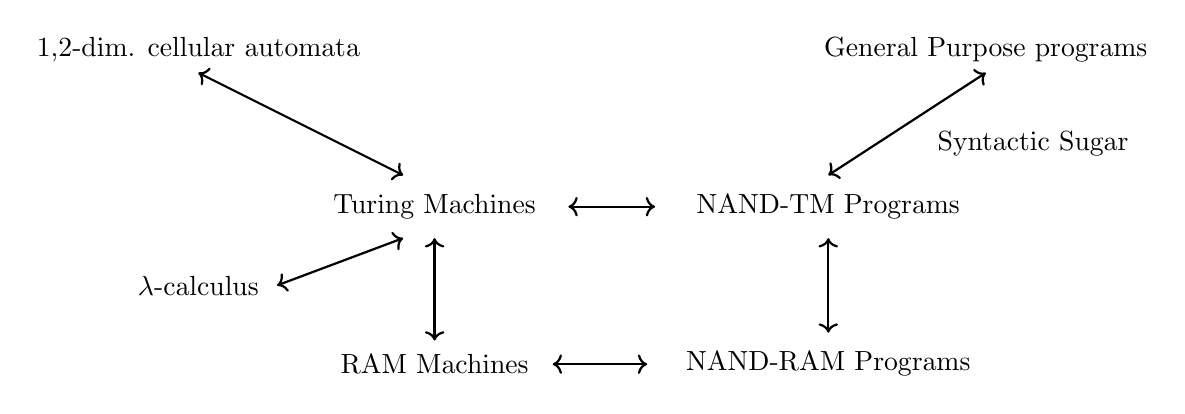
\begin{tikzpicture}
      \node at (0, 0) {Turing Machines};
      \node at (0, -2) {RAM Machines};
      \node at (-3, 2) {1,2-dim. cellular automata};
      \node at (-3, -1) {$\lambda$-calculus};
      \node at (5, -2) {NAND-RAM Programs};
      \node at (5, 0) {NAND-TM Programs};
      \node at (7, 2) {General Purpose programs};
      \node at (7.6, 0.8) {Syntactic Sugar};
      \draw[<->, thick] (-0.4, 0.4)--(-3, 1.7);
      \draw[<->, thick] (-0.4, -0.4)--(-2, -1);
      \draw[<->, thick] (0, -0.4)--(0,-1.7);
      \draw[<->, thick] (1.7, 0)--(2.8,0);
      \draw[<->, thick] (1.5, -2)--(2.7, -2);
      \draw[<->, thick] (5,-0.4)--(5,-1.6);
      \draw[<->, thick] (5, 0.4)--(7, 1.7);
  \end{tikzpicture}
  \end{center}

\section{Universality and Uncomputability}

  It turns out that uniform models such as Turing machines or NAND-TM programs allow us to obtain a truly \textit{universal Turing machine $U$} that can evaluate all other machines, including machines that are more complex than $U$ itself. Similarly, there is a \textit{Universal NAND-TM program $U^\prime$} that can evaluate all NAND-TM programs, including programs that have more lines than $U^\prime$. 

  The existence of such a universal program/machine underlies the technological advances made up to now. Rather than producing special purpose calculating devices such as the abacus, the slide ruler, and machines that compute various trigonometric series, this universal property allows us to build a machine that, via software, can be extended to do arbitrary computations, i.e. a \textit{general purpose computer}. 



  \begin{theorem}[Universal Turing Machine]
  There exists a Turing machine $U$ such that on every string $M$ which represents a Turing machine and $x \in \{0,1\}^*$, 
  \[U(M, x) = M(x)\]
  That is, if the machine $M$ halts on $x$ and outputs some $y \in \{0,1\}^*$, then $U(M, x) = y$ and if $M$ does not halt on $x$ (i.e. $M(x) = \perp$), then $U(M, x) = \perp$. 
  \end{theorem}

  There is more than one Turing machine $U$ that satisfies the theorem above. 

  \begin{definition}[String representation of Turing machine]
  Let $M$ be a Turing machine with $k$ states and size $l$ alphabet
  \[\Sigma = \{\sigma_0, \sigma_1, ..., \sigma_{l-1}\}\]
  (We use the convention $\sigma_0 = 0, \sigma_1 = 1, \sigma_2 = \emptyset, \sigma_3 = \triangleright$. We represent $M$ as the triple $(k, l, T)$, where $T$ is the table of valies for $\delta_M$: 
  \[T = \big(\delta_M (0, \sigma_0), \delta_M (0, \sigma_1), ..., \delta_M (k-1, \sigma_{l-1})\big)\]
  where each value $\delta_M (s, \sigma)$ is a triple $(s^\prime, \sigma^\prime, d)$ with $s^\prime \in [k], \sigma^\prime \in \Sigma$, and $d$ a number in $\{0,1,2,3\}$ encoding one of $\{\mathsf{L, R, S, H}\}$. Thus, such a machine $M$ is encoded by a list of $2 + 3k \cdot l$ natural numbers. The \textbf{string representation} of $M$ is obtained by concatenating prefix-free representations of all these integers. If a string $\alpha \in \{0,1\}^*$ does not represent a list of integers in the form above, then we treat it as representing the trivial Turing machine with one state that immediately halts on every input. 
  \end{definition}
  The big takeways so far are: 
  \begin{enumerate}
      \item We can represent every Turing machine as a string. 
      \item Given the string representation of a Turing machine $M$ and an input $x$, we can simulate $M$'s execution on the input $x$. That is, if we want to simulate a new Turing machine $M$, we do not need to build a new physical machine, but rather can represent $M$ as a string (i.e. using code) and then input $M$ to the universal machine $U$. 
  \end{enumerate}

  \subsection{Uncomputable Functions}
  Even though NAND-CIRC programs can compute every finite function $f: \{0,1\}^n \longrightarrow \{0,1\}$, NAND-TM programs can \textit{not} compute every function $F: \{0,1\}^* \longrightarrow \{0,1\}$. That is, there exists such a function that is \textit{uncomputable}! 

  \begin{definition}
  Let $HALT: \{0,1\}^* \longrightarrow \{0,1\}$ be the function such that for every string $M \in \{0,1\}^*$, $HALT(M, x) = 1$ if Turing machine $M$ halts on the input $x$ and $HALT(M, x) = 0$ otherwise. 
  \end{definition}

  \begin{theorem}
  The $HALT$ function is not computable. This leads to many other functions also being uncomputable. 
  \end{theorem}

  It is surprising that such a simple program is actually uncomputable. That is, there is no \textit{general procedure} that would determine for an \textit{arbitrary} program $P$ whether it halts or not. 

  \subsection{Impossibility of General Software Verification}
  \begin{definition}
  Let there be a program $P$ that computes a function. A \textbf{semantic property} or \textbf{semantic specification} of a program means properties of the \textit{function} that the program computes, as opposed to the properties that depend on the particular syntax/code used by the program. 
  \end{definition}

  \begin{example}
  A semantic property of a program $P$ is the property that whenever $P$ is given an input string with an even number of $1$'s, it outputs $0$. Another example is the property that $P$ will always halt whenever the input ends with a $1$. 

  In contrast the property that a C program contains a comment before every function declaration is not a semantic property, since it depends on the actual source code as opposed to the input/output relation. 
  \end{example}

  \begin{example}
  Consider the following two C programs: 
  \begin{lstlisting}
  int First(int n) {
      if (n<0) return 0; 
      return 2*n;
  }

  int Second(int n) {
      int i = 0;
      int j = 0
      if (n<0) return 0; 
      while (j<n) {
          i = i + 2;
          j= j + 1; 
      }
      return i; 
  }
  \end{lstlisting}
  $\texttt{First}$ and $\texttt{Second}$ are two distinct C programs, but they compute the same function. Therefore, a \textit{semantic property} would either be true for both programs or false for both, since it depends on the function the programs compute. One example of a semantic property is: \textit{The program $P$ computes a function $f$ mapping integers to integers satisfying that $f(n) \geq n$ for every input $n$.} 

  A property is \textit{not semantic} if it depends on the source code rather than the input/output behavior. An example of this would be: \textit{The program contains the variable $\texttt{k}$} or \textit{the program uses the $\texttt{while}$ operation}. 
  \end{example}

  \begin{definition}[Semantic properties]
  A pair of Turing machines $M$ and $M^\prime$ are \textbf{functionally equivalent} if for every $x \in \{0,1\}^*$, $M(x) = M^\prime (x)$ (including when the function outputs $\perp$). 

  A function $F: \{0,1\}^* \longrightarrow \{0,1\}$ is \textbf{semantic} if for every pair of strings $M, M^\prime$ that represent functionally equivalent Turing machines, $F(M) = F(M^\prime)$. Note that we assume that every string represents \textit{some} Turing machine. 
  \end{definition}

  We now present a theorem concerning the Halting problem (the problem of determining whether a Turing machine will halt or not on any arbitrary input). The Halting problem also turns out to be a linchpin of uncomputability. 

  \begin{theorem}[Rice's Theorem]
  Let $F: \{0,1\}^* \longrightarrow \{0,1\}$. If $F$ is semantic and nontrivial, then it is uncomputable. 
  \end{theorem}

  \begin{corollary}
  The following function is uncomputable: 
  \[COMPUTES-PARITY(P) = \begin{cases}1 & P \text{ computes the parity function} \\
  0 & \text{else}
  \end{cases}\]
  \end{corollary}

  Therefore, we can see that the set $\mathbf{R}$ of computable Boolean functions is a proper subset of the set of all functions mapping $\{0, 1\}^* \longrightarrow \{0, 1\}$. 

  \subsection{Context Free Grammars}
  When a person designs a programming language, they need to determine its \textit{syntax}. That is, the designer decides which strings correspond to valid programs, and which ones do not (i.e. which strings contain a syntax error). To ensure that a compiler or interpreter always halts when checking for syntax errors, language designers typically \textit{do not} use a general Turing-complete mechanism to express their syntax. Rather, they use a \textit{restricted} computational model, most often being \textit{context free grammars}. 

  Consider the function $ARITH: \Sigma^* \longrightarrow \{0,1\}$ that takes as input a string $x$ over alphabet 
  \[\Sigma = \{(, ), +, -, \times, \div, 0, 1, 2, 3, 4, 5, 6, 7, 8, 9\}\]
  and returns $1$ if and only if the string $x$ represents a valid arithmetic expression. Intuitively, we build expressions by applying an operation such as $+, -, \times, \div$ to smaller expressions or enclosing them in parentheses. More precisely, we can make the following definitions: 
  \begin{enumerate}
      \item A \textit{digit} is one of the symbols $0, 1, 2, 3, 4, 5, 6, 7, 8, 9$. 
      \item A \textit{number} is a sequence of digits (we will drop the condition that the sequence does not have a leading zero)
      \item An \textit{operation} is one of $+, -, \times, \div$. 
      \item An \textit{expression} has either the form 
      \begin{enumerate}
          \item \textit{"number"}
          \item \textit{"sub-expression1 operation sub-expression2}
          \item \textit{"(sub-expression1)"}
      \end{enumerate}
      where "sub-expression1" and "sub-expression2" are themselves expressions. Note that this is a recursive function. 
  \end{enumerate}
  A context free grammar (CFG) is a formal way of specifying such conditions, consisting of a set of ruels that tell us how to generate strings from smaller components. 

  \begin{definition}[Context Free Grammar]
  Let $\Sigma$ be some finite set. A \textbf{context free grammar (CFG) over $\Sigma$} is a triple $(V, R, s)$ such that: 
  \begin{enumerate}
      \item $V$, known as the \textit{variables}, is a set disjoint from $\Sigma$
      \item $s \in V$ is known as the \textit{initial variable}
      \item $R$ is a set of \textit{rules}. Each rule is a pair $(v, z)$ with $v \in V$ and $z \in (\Sigma \cup V)^*$. We often write the rule $(v, z)$ as 
      \[v \implies z\]
      and say that the string $z$ \textit{can be derived} from the variable $v$. 
  \end{enumerate}
  \end{definition}

  \begin{example}
  The example of well-formed arithmetic expressions can be captured formally by the following context free grammar. 
  \begin{enumerate}
      \item The alphabet $\Sigma$ is $\{(, ), +, -, \times, \div, 0, 1, 2, 3, 4, 5, 6, 7, 8, 9\}$. 
      \item The variables are $V = \{expression, number, digit, operation\}$
      \item The rules are the set $R$ containing the following 19 rules: 
      \begin{enumerate}
          \item 4 Rules: $operation \implies +$, $operation \implies -$, $operation \implies \times$, $operation \implies \div$
          \item 10 Rules: $digit \implies 0$, $digit \implies 1$, ..., $digit \implies 9$
          \item Rule: $number \implies digit$
          \item Rule: $number \implies digit number$
          \item Rule: $expression \implies number$
          \item Rule: $expression \implies expression\; operation\; expression$
          \item Rule: $expression \implies (expression)$
      \end{enumerate}
      \item The starting variable is $expression$.
  \end{enumerate}
  \end{example}

\section{Introduction}

  Up until now, we have been concerned with which functions are computable and which ones are not. But now we will address the finer question of the \textit{time} that it takes to compute functions, as a function of their input length. Time complexity is extremely important to both the theory and practice of computing. 

  Note that the running time of an algorithm is \textit{not} a number. It is a \textit{function} of the length of the input. Informally, we describe \textit{efficient algorithms} as ones that have computational complexity of $O(n^c)$ for a small constant $c$. For some problems we know efficient algorithms and for others the best known algorithms are exponential. It is also interesting that seemingly minor changes in a problem formulation can make the (known) complexity of a problem "jump" from polynomial to exponential. 

  Furthermore, the difference between polynomial vs exponential time is typically \textit{insensitive} to the choice of the particular computational model: a polynomial-time algorithm is still polynomial whether you use Turing machines, RAM machines, or parallel cluster, and similarly an exponential-time algorithm will remain exponential in all of these platforms. 

  \subsection{Finding the shortest path in a graph}
  The \textit{shortest path problem} is the task of finding, given a graph $G = (V, E)$ and two vertices $s, t \in V$, the length of the shortest path between $s$ and $t$ (if such a path exists). That is, we want to find the smallest number $k$ such that there are vertices $v_0, v_1, ..., v_k$ with $v_0 = s, v_k = t$ and for every $i \in \{0,..., k-1\}$ an edge between $v_i$ and $v_{i+1}$. Formally, we define $MINIPATH: \{0,1\}^* \longrightarrow \{0,1\}^*$ to be the function that on input a triple $(G, s, t)$ (represented as a string) outputs the number $k$ which the length of the shortest path in $G$ between $s$ and $t$ or a string representing $\texttt{no path}$ if no such path exists. This algorithm can also yield the actual path itself as a byproduct. 

  If each vertex has at least two neighbors, then there can be an exponential number of paths from $s$ to $t$, but fortunately we do not have to enumerate them all to find the shortest path. We can find the shortest path using a breadth first search (BFS), enumerating $s$’s neighbors, and then neighbors’ neighbors, etc.. in order. If we maintain the neighbors in a list we can perform a BFS in $O(n^2)$ time, while using a \textit{queue} we can do this in $O(m)$ time. Dijkstra’s algorithm is a well-known generalization of BFS to \textit{weighed graphs}, where each edge is given a numerical weight (e.g. the distance between two nodes). 

  \subsubsection{Finding the longest path in a graph}
  The \textit{longest path problem} is the task of finding the length of the \textit{longest} simple (i.e., non-intersecting) path between a given pair of vertices $s$ and $t$ in a given graph $G$. In particular, finding the longest path is a generalization of the famous \textit{Hamiltonian path problem} which asks for a maximally long simple path (i.e., path that visits all $n$ vertices once) between $s$ and $t$, as well as the notorious \textit{traveling salesman problem (TSP)} of finding (in a weighted graph) a path visiting all vertices of cost at most $w$. TSP is a classical optimization problem, with applications ranging from planning and logistics to DNA sequencing and astronomy.

  Surprisingly, while we can find the shortest path in $O(m)$ time, there is no known algorithm for the longest path problem that significantly improves on the trivial “exhaustive search” or “brute force” algorithm that enumerates all the exponentially many possibilities for such paths. Specifically, the best known algorithms for the longest path problem take $O(c^n)$ time for some constant $c > 1$. Currently the best record is $c \approx 1.65$. 

  \subsubsection{Finding the minimum cut in a graph}
  \begin{definition}
  Given a graph $G = (V, E)$, a \textbf{cut} of $G$ is a subset $S \subset V$ such that $S$ is neither empty not is it all of $V$. The edges cut by $S$ are those edges where one of their endpoints is in $S$ and the other is in $\overline{S} = V \setminus S$. We denote this set of edges by $E(S, \overline{S})$. If $s, t \in V$ are a pair of vertices, then an \textbf{$s, t$ cut} is a cut such that $s \in S$ and $t \in \overline{S}$. 
  \end{definition}

  The \textit{minimum $s, t$ cut problem} is the task of finding, given $s, t$, the minimum number $k$ such that there is an $s, t$ cut cutting $k$ edges. This also yields the set $S$ that achieves this minimum. Formally, we define $MINCUT: \{0,1\}^* \longrightarrow \{0,1\}^*$ to be the function that on input a string representing a triple $(G = (V, E), s t)$ of a graph and two vertices, outputs the minimum number $k$ such that there exists a set $S \subset V$ with $s \in S, t \not\in S$, and $|E(S, \overline{S})| = k$. 

  In the diagram below, an example of a cut is labeled with blue, while the minimum $1, 0$ cut is labeled in red. 
  \begin{center}\resizebox{8.1cm}{6.3cm}{%
      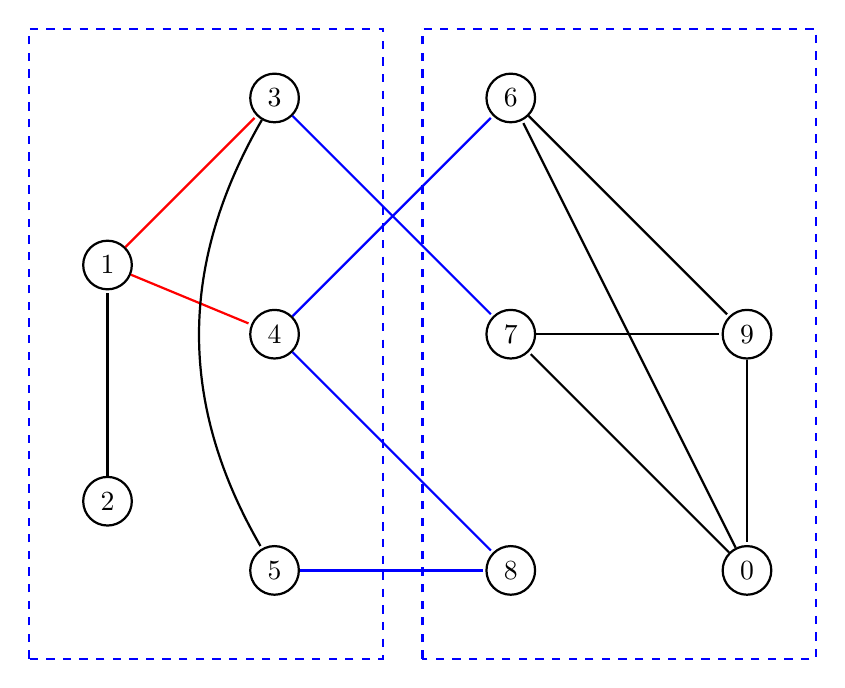
\begin{tikzpicture}[-,>=stealth',shorten >=1pt,auto,node distance=3cm, thick,main node/.style={circle,draw}, every loop/.style={}]
      \node[main node] (1) {1};
      \node[main node] (2) [below of=1] {2};
      \node[main node] (3) [above right of=1] {3};
      \node[main node] (4) [above right of=2] {4};
      \node[main node] (5) [below of=4] {5};
      \node[main node] (6) [right of=3] {6};
      \node[main node] (7) [below of=6] {7};
      \node[main node] (8) [below of=7] {8};
      \node[main node] (9) [right of=7] {9};
      \node[main node] (0) [below of=9] {0};
      \path[every node/.style={font=\sffamily\small}]
      (2) edge node {} (1)
      (1) edge[red] node {} (3)
      (1) edge[red] node {} (4)
      (3) edge[bend right] node {} (5)
      (4) edge[blue] node {} (8)
      (5) edge[blue] node {} (8)
      (4) edge[blue] node {} (6)
      (3) edge[blue] node {} (7)
      (6) edge node {} (9)
      (7) edge node {} (9)
      (9) edge node {} (0)
      (0) edge node {} (6) 
      (0) edge node {} (7);
      \draw[dashed, blue] (-1,-5) rectangle (3.5, 3);
      \draw[dashed, blue] (4, -5) rectangle (9, 3);
      \end{tikzpicture}}
  \end{center}

  There are many applications to computing minimum $s, t$ cuts since minimum cuts often correspond to \textit{bottlenecks}. The applications in communication or railroad networks is obvious now. Additionally, in the setting of image segmentation, one can define a graph whose vertices are pixels and whose edges correspond to neighboring pixels of distinct colors. If we want to separate the foreground from the background, then we can pick (or guess0 a foreground pixel $s$ and a background pixel $t$ and ask for a minimum cut between them. 

  The naive algorithm for computing $MINCUT$ will check all $2^n$ possible subset of an $n$-vertex graph, but we can actually build algorithm that compute $MINCUT$ in polynomial time. 

  \subsubsection{Min-Cut Max-Flow and Linear Programming}
  We can obtain a polynomial-time algorithm for computing $MINCUT$ using the \textit{Max-Flow Min-Cut Theorem}. 

  \begin{theorem}[Max-Flow Min-Cut Theorem]
  In a \textit{flow network} $G$ (we can just interpret this as a weighted directed graph), the maximum amount of flow passing from source $s \in V$ to sink $t \in V$ is equal to the total weight of the edges in a minimum cut. If the graph is unweighted (i.e. every edge has unit capacity), then the maximum flow is just equal to the minimum cut $k$. The \textbf{maximum $s, t$ flow} is the maximum units of water that we could transfer from $s$ to $t$ over these pipes. If there is an $s, t$ cut of $k$ edges, then the maximum flow is at most $k$. 
  \end{theorem}

  It is easy to see why this theorem is when we interpret the minimum cut $S$ acting as a bottleneck that restricts the flow the most. The Max-Flow Min-Cut Theorem reduces the task of computing a minimum cut of the task of computing a \textit{maximum flow}. For this problem, the \textit{Ford-Fulkerson Algorithm} is direct way to compute such a flow using incremental improvements. This is a special case of a more more general tool known as \textit{linear programming}. 

  \begin{definition}
  A \textbf{flow} on a graph $G$ of $m$ edges represents the weight of each edge, which can be interpreted as the amount of water per time-unit that flows through each edge. The flow on this graph of $m$ edges can be modeled as a vector $x \in \mathbb{R}^m$ where for every edge $e, x_e$ corresponds to the amount of water per time-unit that flows on $e$. We think of an edge $e$ as an ordered pair $(u, v)$ (can be chosen arbitrarily) and let $x_e$ be the amount of flow that goes from $u$ to $v$. Since every edge has capacity one, $-1 \leq x_e \leq 1$ for every edge $e$. Finally, a valid flow has the property that the amount of water leaving the source $s$ is the same as the amount entering the sink $t$, and that for every other vertex $v$, the amount of water entering and leaving $v$ is the same. Mathematically, we can write these properties as follows:  
  \begin{align*}
      & \sum_{s} x_s + \sum_t x_t = 0 \\
      & \sum_e x_e = 0 \;\; \forall\; v \in V \setminus \{s, t\} \\
      & -1 \leq x_e \leq 1 & \forall\; e \in E
  \end{align*}
  We write the source and sinks as summations since there may be multiple sources and sinks. 
  \end{definition} 

  \begin{example}
  An example of such a viable sink is: 
  \begin{center}\resizebox{9cm}{5.6cm}{%
      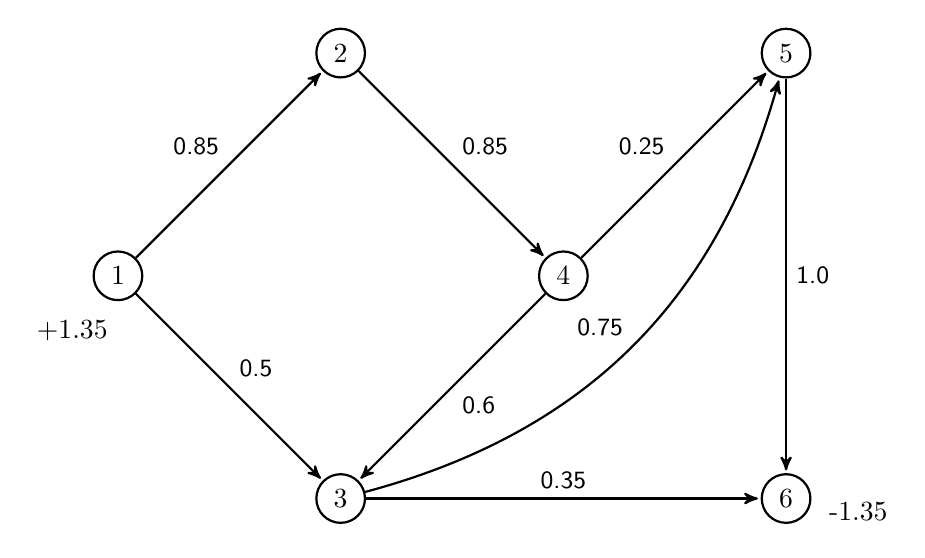
\begin{tikzpicture}[->,>=stealth',shorten >=1pt,auto,node distance=4cm, thick,main node/.style={circle,draw}, every loop/.style={}]
      \node[main node] (1) {1};
      \node[main node] (2) [above right of=1] {2};
      \node[main node] (3) [below right of=1] {3};
      \node[main node] (4) [above right of=3] {4};
      \node[main node] (5) [above right of=4] {5};
      \node[main node] (6) [below right of=4] {6};
      \path[every node/.style={font=\sffamily\small}]
      (1) edge node {0.85} (2)
      (1) edge node {0.5} (3)
      (2) edge node {0.85} (4)
      (4) edge node {0.6} (3)
      (4) edge node {0.25} (5)
      (5) edge node {1.0} (6)
      (3) edge[bend right] node {0.75} (5)
      (3) edge node{0.35} (6);
      \node[left] at (0,-0.7) {+1.35};
      \node[right] at (8.9,-3) {-1.35};
      \end{tikzpicture}}
  \end{center}
  Note that the water flowing from the source and into the sink are both 1.35, and at each node, the water flowing in is equal to the water flowing out. The water flowing through each pipe is also less than 1. 

  From this very simple graph, we can see that the minimum $1, 6$ cut is $k = 2$, and therefore the maximum flow of water from node $1$ to node $6$ is 2 units of water per given time-interval. We can even construct this explicit "maximum flow" as such (there are multiple ways): 
  \begin{center}\resizebox{9cm}{5.6cm}{%
      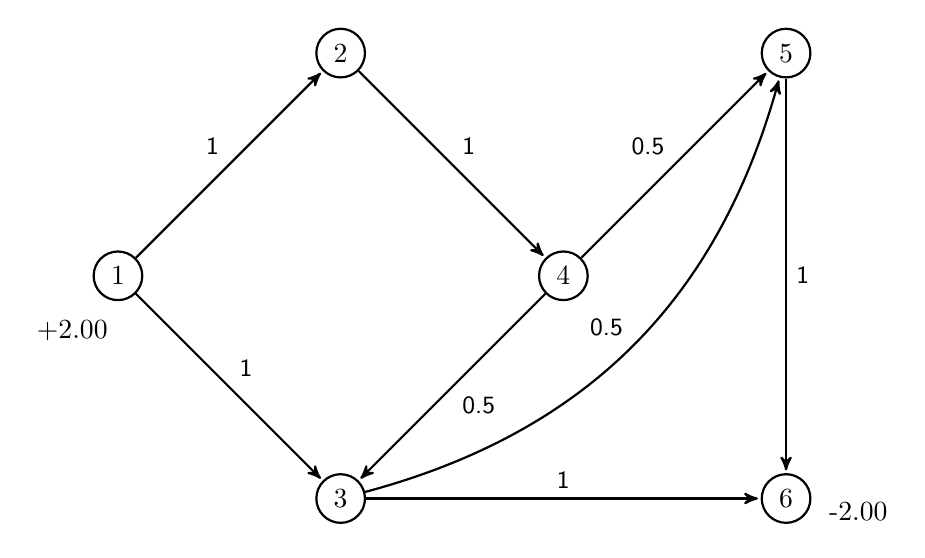
\begin{tikzpicture}[->,>=stealth',shorten >=1pt,auto,node distance=4cm, thick,main node/.style={circle,draw}, every loop/.style={}]
      \node[main node] (1) {1};
      \node[main node] (2) [above right of=1] {2};
      \node[main node] (3) [below right of=1] {3};
      \node[main node] (4) [above right of=3] {4};
      \node[main node] (5) [above right of=4] {5};
      \node[main node] (6) [below right of=4] {6};
      \path[every node/.style={font=\sffamily\small}]
      (1) edge node {1} (2)
      (1) edge node {1} (3)
      (2) edge node {1} (4)
      (4) edge node {0.5} (3)
      (4) edge node {0.5} (5)
      (5) edge node {1} (6)
      (3) edge[bend right] node {0.5} (5)
      (3) edge node{1} (6);
      \node[left] at (0,-0.7) {+2.00};
      \node[right] at (8.9,-3) {-2.00};
      \end{tikzpicture}}
  \end{center}
  \end{example}

  By generalizing this process, the maximum flow problem can be thought of as the task of maximizing $\sum_s x_s$ over all the vectors $x \in \mathbb{R}^m$ satisfying the properties above for graphs. Clearly, the function that maps $l: x \rightarrow x_s$ is linear, and maximizing this linear function $l(x)$ over the set $x \in \mathbb{R}^m$ that satisfy certain linear equalities and inequalities is known as \textit{linear programming}. There are polynomial-time algorithms for solving linear programming, and hence we can solve the maximum flow (and so, minimum cut) problem in polynomial time. In fact, there are much better algorithms for maximum flow/minimum-cut, even for weighted directed graphs, with the record standing at $O(\min\{m^{10/7}, m\sqrt{n}\})$ time. 

  \begin{definition}
  Given a graph $G = (V, E)$, the \textbf{\textit{global} minimum cut} of $G$ is the minimum over \textit{all} $S \subset V$ with $S \neq \emptyset, V$ of the number of edges cut by $S$. Therefore, the points $s, t$ are not chosen initially, and every graph has a global minimum cut. 
  \end{definition}

  \begin{theorem}
  There is a polynomial-time algorithm to compute the global minimum cut of a graph. 
  \end{theorem}

  Similarly, the \textit{maximum cut} problem is the task of finding, given an input graph $G = (V, E)$, the subset $S \subset V$ that \textit{maximizes} the number of edges cut by $S$. This can also be defined for the $s, t$ cut, too. But unlike the minimum cut problem which can be solved using a polynomial time-algorithm, there is no known algorithm solving maximum cut much faster than the trivial "brute force" algorithm that tries all $2^n$ possibilities for the set $S$. 

  \subsubsection{Convexity}
  There is an underlying reason for the difference between the difficulty of maximizing and minimizing a function over a domain. If $D \subset \mathbb{R}^m$, then a function $f: D \longrightarrow R$ is \textit{convex} if for every $x, y \in D$ and $p \in [0,1]$, 
  \[f(px + (1-p)y) \leq p f(x) + (1-p) f(y)\]

  \begin{theorem}
  Given a convex set $D \subset \mathbb{R}^m$ and convex function $f: D \longrightarrow R$, if $x$ is a local minimum of $f$, then it is also a global minimum. 
  \end{theorem}
  \begin{proof}
  Assume that $x$ is the local minimum and there is a global minimum $y \neq x$. $f(y) < f(x)$, so every point $z = px + (1-p) y$ on the line segment between $x$ and $y$ will satisfy 
  \[f(z) \leq p f(x) + (1-p) f(y) < f(x)\]
  and hence in particular $x$ cannot be a local minimum. 
  \end{proof}

  In general, local minima of functions are much easier to find than global ones (e.g. using algorithms like gradient descent). Indeed, under certain technical conditions, we can often efficiently find the minimum of convex functions over a convex domain, and this is the reason why problems such as minimum cut and shortest path are easy to solve. On the other hand, maximizing a convex function over a convex domain (or equivalently, minimizing a concave function) can often be a hard computational task. A linear function is both convex and concave, which is the reason that both the maximization and minimization problems for linear functions can be done efficiently.

  The minimum cut problem is not a priori a convex minimization task, because the set of potential cuts is discrete and not continuous. However, it turns out that we can embed it in a continuous and convex set via the (linear) maximum flow problem. The “max flow min cut” theorem ensures that this embedding is “tight” in the sense that the minimum “fractional cut” that we obtain through the maximum-flow linear program will be the same as the true minimum cut. Unfortunately, we don’t know of such a tight embedding in the setting of the maximum cut problem. 

  \subsection{Computational Problems Beyond Graphs}
  \subsubsection{SAT}
  A \textbf{propositional formula} $\varphi$ involves $n$ variables $x_1, x_2, ..., x_n$ and the logical operators AND ($\wedge$), OR ($\vee$), and NOT ($\neg$, also denoted with a bar). 

  \begin{definition}
  We say that a propositional formula is in \textit{conjunctive normal form (CNF)} if it is an AND of ORs or their negations. A term of the form $x_i$ or $\overline{x_i}$ is called a \textbf{literal}. 

  Furthermore, we say that a formula is a \textbf{k-CNF} if it is an AND of ORs where each OR involves exactly $k$ literals. 
  \end{definition}

  \begin{example}
  This is a CNF formula since it is an AND of ORs of literals. 
  \[(x_7 \vee \overline{x_{22}} \vee x_{15}) \wedge (x_{37} \vee x_{22}) \wedge (x_{55} \vee \overline{x_7})\]
  \end{example}

  \begin{definition}
  A \textbf{satisfying assignment} for CNF formula $\varphi$ is a string $x \in \{0,1\}^*$ such that $\varphi$ evaluates to \textit{True} if we assign its variables the values of $x$. 
  \end{definition}

  Following this, the \textbf{satisfiability problem} is the task of determining, given a CNF formula $\varphi$, whether or not there exists a satisfying assignment for $\varphi$. More specifically, the $k$-SAT problem is the restriction of the satisfiability problem for the case that the input formula is a $k$-CNF. 

  \begin{example}
  The CNF formula 
  \[(x_1 \vee \overline{x_2}) \wedge (\overline{x_1} \vee x_2 \vee x_3) \wedge \overline{x_1}\]
  is satisfiable by assigning $x = (x_1, x_2, x_3) = (FALSE, FALSE, arbitrary)$, since 
  \begin{align*}
      & (FALSE \vee \overline{FALSE}) \wedge (\overline{FALSE} \vee FALSE \vee x_3) \wedge \overline{FALSE} \\
      = & (FALSE \vee TRUE) \wedge (TRUE \vee FALSE \vee x_3) \wedge TRUE \\
      = & TRUE \wedge TRUE \wedge TRUE \\
      = & TRUE
  \end{align*}
  However, the CNF formula 
  \[x_1 \wedge \overline{x_1}\]
  is not satisfiable, since neither $x_1 = TRUE$ nor $x_1 = FALSE$ will reduce the above statement to TRUE. 
  \end{example}

  The trivial, brute-force algorithm for \textbf{2SAT} will enumerate all the $2^n$ assignments $x \in \{0,1\}^n$ but fortunately, we can do much better. Let us assume that there exists a satisfiable solution to this 2-CNF formula. Then, we can think of every constraint $l_i \vee l_j$ (where $l_i, l_j$ are literals, corresponding to variables or their negations) as an \textit{implication} $\overline{l_i} \implies l_j$, since if $l_i$ is false then $l_j$ must be true. Therefore, we can make a directed graph of the $2n$ literals ($x_1, ..., x_n, \overline{x_1}, ..., \overline{x_n}$) with every constraint $l_i \vee l_j$ corresponding to the directed edge $\overline{l_i} \rightarrow l_j$. With this, it can be shown that $\varphi$ is unsatisfiable if and only if there is a variable $x_i$ such that there is a directed path from $x_i$ to $\overline{x_i}$ and from $\overline{x_i}$ to $x_i$ (since this means that $x_i \implies... \implies \overline{x_i}$, reaching a contradiction). 

  The \textbf{3SAT} problem is the task of determining satisfiability for $3$-CNFs, and we do not know of a significantly better than brute force algorithm for 3SAT. The best known algorithms take roughly $1.3^n$ steps. 

  \subsubsection{Solving Linear and Quadratic Equations}
  The standard Gaussian elimination algorithm can be used to solve a linear system of $n$ equations in $n$ variables in polynomial time. In fact, if we are willing to allow some loss in precision, there are algorithms that can handle linear \textit{inequalities}, also known as linear programming. In contrast, if we would like \textit{integer solutions}, the ask for solving linear equalities or inequalities is known as \textit{integer programming}, and the best known algorithms are exponential time in the worst case. 

  However, if we would like to solve not just linear but equations involving quadratic terms of the form 
  \[a_{i, j} x_j x_k\]
  That is, suppose that we are given a set of quadratic polynomials $p_1, ..., p_m$ and consider the homoegeneous equations $p_i (x) = 0$. To avoid issues with bit representations, we will always assume that the equations contain the constraints $x_i^2 - x_i = 0$ (with only solutions being $x_i = 0, 1$). This means that we can restrict attention to solutions in $\{0,1\}^n$. For this problem, we do not know a much better algorithm for this problem than the one that enumerates over all the $2^n$ possibilities. 

  \subsubsection{Determinant and Permanent of a Matrix}
  Using the LUP decomposition algorithm (which is really dependent on polynomial-time Gaussian elimination), the determinant of an $n \times n$ matrix can be computed in polynomial time of arithmetic operations. 

  \begin{definition}
  The \textbf{permanent} of $n \times n$ matrix $A$ is defined as
  \[\text{perm}(A)= \sum_{\sigma \in S_n} \prod_{i=1}^n A_{i, \sigma(i)}\]
  That is, perm$(A)$ is defined analogously to the determinant except that we drop the sign of $\sigma$. 
  \end{definition}

  It turns out that we can find compute a function perm$_2 (A)$ that computes the permanent modulo 2 in polynomial time, but as soon as we reach permanent modulo 3 or greater prime numbers, we do not know of a much better than brute force algorithm to even compute the permanent modulo 3. 

  \subsubsection{Finding a Zero-Sum Equilibrium}

  \begin{definition}
  A \textbf{zero sum game} is a game between two players where the payoff for one is the same as the penalty for the other. A zero sum game can be specified by a $n \times n$ matrix $A$, where if player chooses action $i$ and player 2 chooses action $j$ then player one gets $A_{i, j}$ and player 2 loses the same amount. 
  \end{definition}

  The famous \textit{Min Max theorem} of linear algebra states that we if allow probabilistic or mixed strategies (where a player does not choose a single action but rather a \textit{distribution} over actions), then it does not matter who plays first and the end result will be the same. Mathematically, the min max theorem is that if we let $\delta_n$ be the set of probability distributions over $[n]$ (i.e. $\delta_n$ is the set of all nonnegative column vectors in $\mathbb{R}^n$ whose entries sum up to $1$), then 
  \[\max_{p \in \delta_n} \; \min_{q \in \delta_n} p^T A q = \min_{q \in \delta_n} \; \max_{p \in \delta_n} p^T A q\]
  This value can be computed efficiently by a linear program. 

  \subsubsection{Finding a Nash Equilibrium}
  For games that are not zero sum, where the payoff of one player does not necessarily equal the loss of the other, there is the notion of a \textit{Nash equilibrium} for such games as well. However, unlike zero sum games, we do not know of an efficient algorithm for finding a Nash equilibrium given the description of a general (non zero-sum) game. In particular, this means that there are games for which natural strategies will take an exponential number of steps to converge to an equilibrium. 

  \subsubsection{Primality Testing and Integer Factoring}
  In order to determine whether a number $N$ is prime or not, we can try dividing it by all the numbers up to $\sqrt{N}$, but this is still quite terrible computationally. But fortunately, a \textit{probabilistic} algorithm to determine whether a given number $N$ is prime or composite in time $poly(n)$ for $n = \log N$. 

  On the contrary, no such algorithm that could efficiently find the factorization of $N$ is known. 

  \subsection{Current Knowledge}
  The difference between an exponential and polynomial time algorithms might seem merely “quantitative” but it is in fact extremely significant. As we’ve already seen, the brute force exponential time algorithm runs out of steam very very fast, and in practice there might not be much difference between a problem where the best algorithm is exponential and a problem that is not solvable at all. Thus the efficient algorithms we mentioned above are widely used and power many computer science applications. Moreover, a polynomial-time algorithm often arises out of significant insight to the problem at hand, whether it is the max-flow min-cut result, the solvability of the determinant, or the group theoretic structure that enables primality testing. Such insight can be useful regardless of its computational implications. 

  At the moment we do not know whether the “hard” problems are truly hard, or whether it is merely because we haven’t yet found the right algorithms for them. However, we will now see that there are problems that do inherently require exponential time. We just don’t know if any of the examples above fall into that category. 

\section{Modeling Running Time}

  When talking about running time, what we care about is the \textit{scaling behavior} of the number of steps as the input size grows (as opposed to a fixed number). 

  \subsection{Formally Defining Running Time}
  We can informally define what it means for a function $F: \{0,1\}^* \longrightarrow \{0,1\}^*$ to be \textit{computable} in time $T(n)$ steps, where $T$ is some function mapping the length $n$ of the input to the number of computation steps allowed. 

  \begin{definition}
  Let $T: \mathbb{N} \longrightarrow \mathbb{N}$ be some function. We say that a function $F: \{0,1\}^* \longrightarrow \{0,1\}^*$ is \textbf{computable in $T(n)$ Turing Machine time (TM-time for short)} if there exists a Turing machine $M$ such that for every sufficiently large $n$ and every $x \in \{0,1\}^n$, the machine halts after executing at most $T(n)$ steps and outputs $F(x)$. 

  We define $TIME_{\mathsf{TM}}\big(T(n)\big)$ to be the set of Boolean functions ($\{0,1\}^* \longrightarrow \{0,1\}$) that are computable in $T(n)$ TM time. Note that $TIME_{\mathsf{TM}}\big(T(n)\big)$ is a class of \textit{functions}, not machines. 
  \end{definition}

  With this, we can formally define what is means for function $F: \{0,1\}^* \longrightarrow \{0,1\}$ to be computable in time at most $T(n)$ where $n$ is the size of the input. Furthermore, the property of considering only "sufficiently large" $n$'s is not very important but it is convenient since it allows us to avoid dealing explicitly with uninteresting "edge cases." We have also defined computability with Boolean functions for simplicity, but we can generalize this further. 

  \subsubsection{Polynomial and Exponential Time}
  \begin{definition}
  The two main time complexity classes are defined: 
  \begin{enumerate}
      \item \textbf{Polynomial time}: A function $F: \{0,1\}^* \longrightarrow \{0,1\}$ is \textbf{computable in polynomial time} if it is in the class
      \[\mathbf{P} = \bigcup_{c \in \{1, ...m\}} TIME_{\mathsf{TM}} \big( n^c \big), \;\;\; m \in \mathbb{N}\]
      That is, $F \in \mathbf{P}$ if there is an algorithm to compute $F$ that runs in time at most \textit{polynomial} in the length of the input. 
      \item \textbf{Exponential time}: A function $F: \{0,1\}^* \longrightarrow \{0,1\}$ is \textbf{computable in exponential time} if it is in the class 
      \[\mathbf{EXP} = \bigcup_{c \in \{1, ..., m\}} TIME_{\mathsf{TM}} \big( 2^{n^c}\big)\]
      That is, $F \in \mathbf{EXP}$ if there is an algorithm to compute $F$ that runs in time at most \textit{exponential} in the length of the input. 
  \end{enumerate}
  Summarizing this, we say that $F \in \mathbf{P}$ if there is a polynomial $p: \mathbb{N} \longrightarrow \mathbb{R}$ and a Turing machine $M$ such that for every $x \in \{0,1\}^*$, when given input $x$, the Turing machine halts within at most $p(|x|)$ steps and outputs $F(x)$. 

  We say that $F \in \mathbf{EXP}$ if there is a polynomial $p: \mathbb{N} \longrightarrow \mathbb{R}$ and a Turing machine $M$ such that for every $x \in \{0,1\}^*$, when given input $x$, $M$ halts within at most $2^{p(|x|)}$ steps and outputs $F(x)$. 
  \end{definition}

  \begin{lemma}
  Since exponential time is much larger than polynomial time, 
  \[\mathbf{P} \subset \mathbf{EXP}\]
  \end{lemma}

  Time complexity for the previous algorithms are as follows: 
  \begin{center}
  \begin{tabular}{l|l}
      \textbf{P} & \textbf{EXP} (not known to be \textbf{P}) \\
      \hline
      Shortest path & Longest path \\
      Min cut & Max cut \\
      2SAT & 3SAT \\
      Linear eqs & Quad eqs \\
      Zerosum & Nash \\
      Determinant & Permanent\\
      Primality & Factoring
  \end{tabular}
  \end{center}
  Many technological developments are centered around these facts. For example, the exponential time complexity of factoring algorithms is what makes the RSA-encryption so secure. If a polynomial time algorithm for factoring were to be discovered, RSA-encryption would be rendered obsolete. 

  \subsection{Modeling Running Time Using RAM Machines/NAND-RAM}
  Despite the theoretical elegance of Turing machines, RAM machines and NAND-RAM programs are much more closely related to actual computing architecture. For example, even a "merge sort" program cannot be implemented on a Turing machines in $O(n \log n)$ time. We can define running time with respect to NAND-RAM programs just as we did for Turing machines. 

  \begin{definition}
  Let $T: \mathbb{N} \longrightarrow \mathbb{N}$. We say that a function $F: \{0,1\}^* \longrightarrow \{0,1\}^*$ is \textbf{computable in $\mathbf{T(n)}$ RAM time (RAM-time for short)} if there exists a NAND-RAM program $P$ such that for every sufficiently large $n$ and every $x \in \{0,1\}^n$, when given input $x$, the program $P$ halts after executing at most $T(n)$ lines and outputs $F(x)$. 

  We define $TIME_{\mathsf{RAM}} \big(T(n)\big)$ to be the set of Boolean functions ($\{0,1\}^* \longrightarrow \{0,1\}$) that are computable in $T(n)$ RAM time. 
  \end{definition}

  We will use $TIME \big( T(n)\big)$ to denote $TIME_{\mathsf{RAM}} \big(T(M) \big)$. However, as long as we only care about the difference between exponential and polynomial time, the model of running time we use does not make much difference. The reason is that Turing machines can simulate NAND-RAM programs with at most a polynomial overhead. 

  \begin{theorem}[Relating RAM and Turing machines]
  Let $T: \mathbb{N} \longrightarrow \mathbb{N}$ be a function such that $T(n) \geq n$ for every $n$ and the map $n \mapsto T(n)$ can be computed by a Turing machine in time $O(T(n))$. Then, 
  \[TIME_{\mathsf{TM}}\big( T(n)\big) \subseteq TIME_{\mathsf{RAM}}\big( 10 \cdot T(n)\big) \subseteq TIME_{\mathsf{TM}} \big( T(n)^4\big)\]
  We can visually see this classification as 
  \begin{center}
  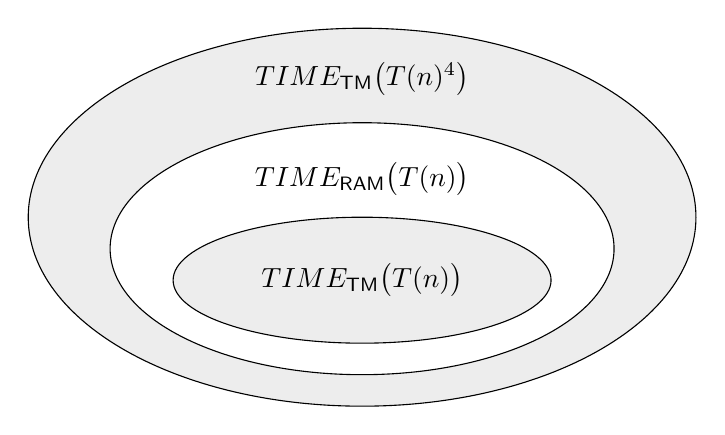
\begin{tikzpicture}[scale=0.8]
      \draw[fill=lightgray] (0,1) ellipse (5.3 and 3);
      \draw[fill=white] (0,0.5) ellipse (4 and 2);
      \draw[fill=lightgray] (0,0) ellipse (3 and 1);
      \node at (0,0) {$TIME_{\mathsf{TM}}\big(T(n)\big)$};
      \node at (0,1.6) {$TIME_{\mathsf{RAM}}\big(T(n)\big)$};
      \node at (0,3.2) {$TIME_{\mathsf{TM}}\big(T(n)^4\big)$};
  \end{tikzpicture}
  \end{center}
  \end{theorem}

  With this, we could have equally defined $\mathbf{P}$ as the class of functions computable by NAND-RAM programs (instead of Turing machines) that run in polynomial time in the length of the input. Similarly, with $T(n) = 2^{n^a}$, we see that the class $\mathbf{EXP}$ can also be defined as the set of functions computable by NAND-RAM programs in time at most $2^{p(n)}$ where $p$ is some polynomial. This justifies the choice of $\mathbf{P}$ as capturing a technology-independent notion of tractability. Therefore, \textit{all "reasonable" computational models are equivalent if we only care about the distinction between polynomial and exponential}, with reasonable referring to all scalable computational models that have been implemented except possibly quantum computers. 

  When considering general time bounds, we need to make sure to rule out some "exceptional" cases such as functions $T$ that don't give enough time for the algorithm to even read the input, or functions where the time bound itself is uncomputable. More precisely, $T$ must be a \textit{nice function}. 

  \begin{definition}
  That is why we say that the function $T: \mathbb{N} \longrightarrow \mathbb{N}$ is a \textbf{nice time bound function} (\textbf{nice function} for short) if 
  \begin{enumerate}
      \item for every $n \in \mathbb{N}$ $T(n) \geq n$ ($T$ allows enough time to read the input)
      \item for every $n^\prime \geq n$, $T(n^\prime) \geq T(n)$ ($T$ allows more time on longer inputs)
      \item the map $F(x) = 1^{T(|x|)}$ (i.e. mapping a string of length $n$ to a sequence of $T(n)$ ones) can be computed by a NAND-RAM program in $O(T(n))$ time
  \end{enumerate}
  \end{definition}

  So, the following are examples of polynomially equivalent models: 
  \begin{enumerate}
      \item Turing machines
      \item NAND-RAM programs/RAM machines
      \item All standard programming languages, including C/Python/Javascript...
      \item The $\lambda$ calculus
      \item Cellular automata
      \item Parallel computers
      \item Biological computing devices such as DNA-based computers 
  \end{enumerate}

  The \textit{Extended Church Turing Thesis} is the statement that this is true for all physically realizable computing models. In other words, the extended Church Turing thesis says that for every \textit{scalable computing device} $C$ (which has a finite description but can be in principle used to run computation on arbitrarily large inputs), there is some constant $a$ such that for every function $F: \{0,1\}^* \longrightarrow \{0,1\}$ that $C$ can compute on $n$ length inputs using an $S(n)$ amount of physical resources. This is a strengthening of the plain Church Turing Thesis, which states that the set of computable functions is the same for all physically realizable models, but without requiring the overhead in the simulation between different models to be at most polynomial. 

  Like the Church-Turing thesis itself, the extended Church-Turing thesis is in the asymptotic setting and does not directly yield an experimentally testable prediction. However, it can be instantiated with more concrete bounds on the overhead, yielding experimentally- testable predictions such as the Physical Extended Church-Turing Thesis. 
   
  \subsection{Efficient Universal Machine: A NAND-RAM Interpreter in NAND-RAM}
  We can now see that the universal Turing machine $U$, which can compute every Turing machine $M$, has a \textit{polynomial} overhead for simulating a $NAND-TM$ program. That is, it can simulate $T$ steps of a given $NAND-TM$ (or $NAND-RAM$) program $P$ on an input $x$ in $O(T^4)$ steps. But in fact, by directly simulating $NAND-RAM$ programs we can do better with only a \textit{constant} multiplicative overhead. 

  \begin{theorem}[Efficient Universality of NAND-RAM]
  There exists a NAND-RAM program $U$ satisfying the following: 
  \begin{enumerate}
      \item \textit{U is a universal NAND-RAM program}: For every NAND-RAM program $P$ and input $x$, $U(P, x) = P(x)$ where by $U(P, x)$ we denote the output of $U$ on a string encoding the pair $(P, x)$. 
      \item \textit{U is efficient}: There are some constants $a, b$ such that for every $NAND-RAM$ program $P$, if $P$ halts on input $x$ after most $T$ steps, then $U(P, x)$ halts after at most $C \cdot T$ steps where $C \leq a |P|^b$. 
  \end{enumerate}
  \end{theorem}

  This leads to a corollary. Given any Turing machine $M$, input $x$, and \textit{step budget} $T$, we can simulate the execution for $M$ for $T$ steps in time that is polynomial in $T$. Formally, we define a function $TIMEDEVAL$ that takes the three parameters $M, x$, and the time budget, and outputs $M(x)$ if $M$ halts within at most $T$ steps, and outputs $0$ otherwise. That is, let $TIMEDEVAL: \{0,1\}^* \longrightarrow \{0,1\}^*$ be the function defined as 
  \[TIMEDEVAL (M, x, 1^T) = \begin{cases}
  M(x) & M \text{ halts within } \leq T \text{ steps on } x \\
  0 & \text{else}
  \end{cases}\]
  Then, $TIMEDEVAL \in \mathbf{P}$, i.e. the timed universal Turing machine computes $TIMEDEVAL$ in polynomial time. 

  \subsection{The Time Hierarchy Theorem}
  Some functions are uncomputable, but are there functions that can be computed, but only at an exorbitant cost? For example, is there a function that \textit{can} be computed in time $2^n$, but \textit{cannot} be computed in time $2^{0.9 n}$? It turns out that the answer is yes. 

  \begin{theorem}[Time Hierarchy Theorem]
  For every nice function $T: \mathbb{N} \longrightarrow \mathbb{N}$, there is a function $F: \{0,1\}^* \longrightarrow \{0,1\}$ in 
  \[TIME \big( T(n) \log n\big) \setminus TIME \big( T(n)\big) \]
  There is nothing special about $\log n$. We could have used any other efficiently computable function that ends to infinity with $n$. 
  \end{theorem}

  \subsection{Non-Uniform Computation}

\section{Polynomial-Time Reductions}

  Let us redefine some of the problems into \textit{decision problems}. 

  \textbf{3SAT} The \textit{3SAT problem} can be phrased as the function $3SAT: \{0,1\}^* \longrightarrow \{0,1\}$ that takes as an input a 3CNF formula $\varphi$ (i.e. a formula of the form $C_0 \wedge ... \wedge C_{m-1}$ where each $C_i$ of the OR of three iterables) and maps $\varphi$ to $1$ if there exists some assignment to the variables of $\varphi$ that causes it to evaluate to \textit{true} and to $0$ otherwise. For example, 
  \[3SAT \big( (x_0 \vee \overline{x_1} \vee x_2) \wedge (x_1 \vee x_2 \vee \overline{x_3}) \wedge (\overline{x_0} \vee \overline{x_2} \vee x_3) \big) = 1\]
  since the assignment $x = 1101$ satisfies the input formula. 

  \textbf{Quadratic Equations} The \textit{quadratic equations problem} corresponds to the function $QUADEQ: \{0,1\}^* \longrightarrow \{0,1\}$ that maps a set of quadratic equations $E$ to $1$ if there is an assignment $x$ that satisfies all equations and to $0$ otherwise. 

  \textbf{Longest Path} The \textit{longest path problem} correpsonds to the function $LONGPATH: \{0,1\}^* \longrightarrow \{0,1\}^*$ that maps a graph $G$ and a number $k$ to $1$ if there is a simple path in $G$ of length at least $k$, and maps $(G, k)$ to $0$ otherwise. 

  \textbf{Maximum Cut} The \textit{maximum cut problem} corresponds to the function $MAXCUT: \{0,1\}^* \longrightarrow \{0,1\}$ that maps a graph $G$ and a number $k$ to $1$ if there is a cut in $G$ that cuts at least $k$ edges, and maps $(G, k)$ to $0$ otherwise. 

  All of these problems above are in \textbf{EXP} but it is not known whether or not they are in \textbf{P}. However, we can reduce these problems to ones that are in \textbf{P}, proving that they are indeed in \textbf{P}. 

  \subsection{Polynomial-Time Reductions}
  Suppose that that $F, G: \{0,1\}^* \longrightarrow \{0,1\}$ are two Boolean functions. A \textit{polynomial-time reduction} (or \textit{reduction}) from $F$ to $G$ is a way to sho that $F$ is "no harder" than $G$ in the sense that a polynomial-time algorithm for $G$ implies a polynomial-time algorithm for $F$. 

  \begin{definition}[Polynomial-time reductions]
  Let $F, G: \{0,1\}^* \longrightarrow \{0,1\}$. We say that \textbf{F reduces to G}, denoted by $F \leq_p G$, if there is a polynomial-time computable $R: \{0,1\}^* \longrightarrow \{0,1\}^*$ such that for every $x \in \{0,1\}^*$, 
  \[F(x) = G \big(R(x)\big)\]
  We say that $F$ and $G$ have \textbf{equivalent complexity} if $F \leq_p G$ and $G \leq_p F$. Clearly, $\leq_p$ is a transitive property. 
  \end{definition}

  \subsection{Reducing 3SAT to Zero-One and Quadratic Equations}
  \begin{definition}
  The \textbf{Zero-One Linear Equations problem} corresponds to the function 
  \[01EQ: \{0,1\}^* \longrightarrow \{0,1\}\]
  whose input is a collection $E$ of linear equations in variables $x_0, ..., x_{n-1}$, and the output is $1$ iff there is an assignment $x \in \{0,1\}^n$ satisfying the matrix equation
  \[A x = b, \;\; A \in \text{Mat}(m \times n, \{0,1\}), b \in \mathbb{N}^m\]
  For example, if $E$ is a string encoding the set of equations
  \begin{align*}
      x_0 + x_1 + x_2 & = 2 \\
      x_0 + x_2 = 1 \\
      x_1 + x_2 = 2
  \end{align*}
  then $01EQ(E) = 1$ since the assignment $x = 011$ satisfies all three equations.  
  \end{definition}

  Note that if we extended the field to $\mathbb{R}$, then this can be solved using Gaussian elimination in polynomial time, but there is no known efficiently algorithm to solve $01EQ$. This is stated in the following theorem. 

  \begin{theorem}[Hardness of 01 Linear Equations]
  \[3SAT \leq_p 01EQ\]
  \end{theorem}

  This means that finding an efficient algorithm to solve $01EQ$ would imply an algorithm for $3SAT$. We can further use this to reduce $3SAT$ to the quadratic equations problem, where $QUADEQ(p_0, ..., p_{m-1}) = 1$ if and only if there is a solution $x \in \mathbb{R}^n$ to the equations $p_i (x) = 0$ for $i = 0, ..., m-1$. For example, the following is a set of quadratic equations over the variables $x_0, x_1, x_2$: 
  \begin{align*}
      x_0^2 - x_0 = 0 \\
      x_1^2 - x_1 = 0 \\
      x_2^2 - x_2 = 0 \\
      1 - x_0 - x_1 + x_0 x_1 = 0
  \end{align*}

  \begin{theorem}[Hardness of Quadratic Equations]
  \[3SAT \leq_p QUADEQ\]
  \end{theorem}

  \subsection{Independent Set and Other Graph Problems}
  \begin{definition}
  For a graph $G = (V, E)$, an \textbf{independent set}, also known as a \textbf{stable set}, is a subset $S \subseteq V$ such that there are no edges with both endpoints in $S$ (in other words, $E(S, S) = \emptyset$). Trivially, every singleton (of one point) is an independent set. 
  \end{definition}

  The \textbf{maximum independent set} problem is the task of finding the largest independent set in the graph. The independent set problem is naturally related to \textit{scheduling problem}: if we put an edge between two conflicting tasks, then an independent set corresponds to a set of tasks that can all be scheduled together without conflicts. 

  \begin{theorem}[Hardness of Independent Set]
  \[3SAT \leq_p ISET\]
  \end{theorem}

  \begin{definition}
  A \textbf{vertex cover} in a graph $G = (V, E)$ is a subset $S \subseteq V$ of vertices that touches all edges of $G$. For example, the following blue nodes is a vertex cover of the graph. 
  \begin{center}\resizebox{5cm}{5.6cm}{%
      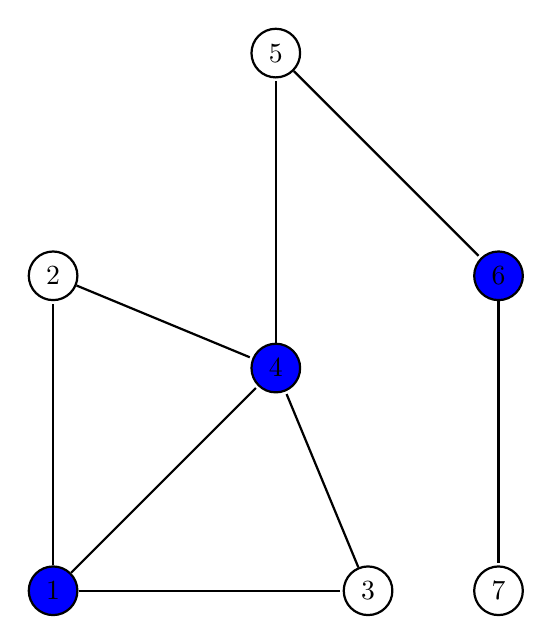
\begin{tikzpicture}[-,>=stealth',shorten >=1pt,auto,node distance=4cm, thick,main node/.style={circle,draw}, every loop/.style={}]
      \node[main node, fill=blue] (1) {1};
      \node[main node] (2) [above of=1] {2};
      \node[main node] (3) [right of=1] {3};
      \node[main node, fill=blue] (4) [above right of=1] {4};
      \node[main node] (5) [above of=4] {5};
      \node[main node, fill=blue] (6) [below right of=5] {6};
      \node[main node] (7) [below of=6] {7};
      \path[every node/.style={font=\sffamily\small}]
      (1) edge node {} (2)
      (1) edge node {} (3)
      (1) edge node {} (4)
      (2) edge node {} (4)
      (3) edge node {} (4)
      (4) edge node {} (5)
      (5) edge node {} (6)
      (6) edge node {} (7);
      \end{tikzpicture}}
  \end{center}

  The \textbf{vertex cover problem} is the task to determine, given a graph $G$ and a number $k$, whether there exists a vertex cover in the graph with at most $k$ vertices. Formally, this is the function 
  \[VC: \{0,1\}^* \longrightarrow \{0,1\}\]
  such that for every $G = (V, E)$ and $k \in \mathbb{N}$, $VC(G, k) = 1$ if and only if there exists a vertex cover $S \subset V$ such that $|S| \leq k$. 
  \end{definition}

  \begin{theorem}
  \[3SAT \leq_p VC\]
  \end{theorem}

  \begin{definition}
  A \textbf{clique} is a subset of vertices of an undirected graph such that every two distinct vertices in the graph are adjacent, i.e. connected by an edge. 

  The \textbf{maximum clique problem} corresponds to the function 
  \[CLIQUE: \{0,1\}^* \longrightarrow \{0,1\}\]
  such that for a graph $G$ and a number $k$, $CLIQUE(G, k) = 1$ iff there is a subset $S$ of $k$ vertices such that for \textit{every} distinct $u, v \in S$, the edge $u, v$ is in $G$. For example, in the graph below, the left subset of 4 vertices is indeed a clique, while the right subset of 4 is not since the edge connecting $6$ to $7$ is not present. 
  \begin{center}\resizebox{12cm}{5cm}{%
      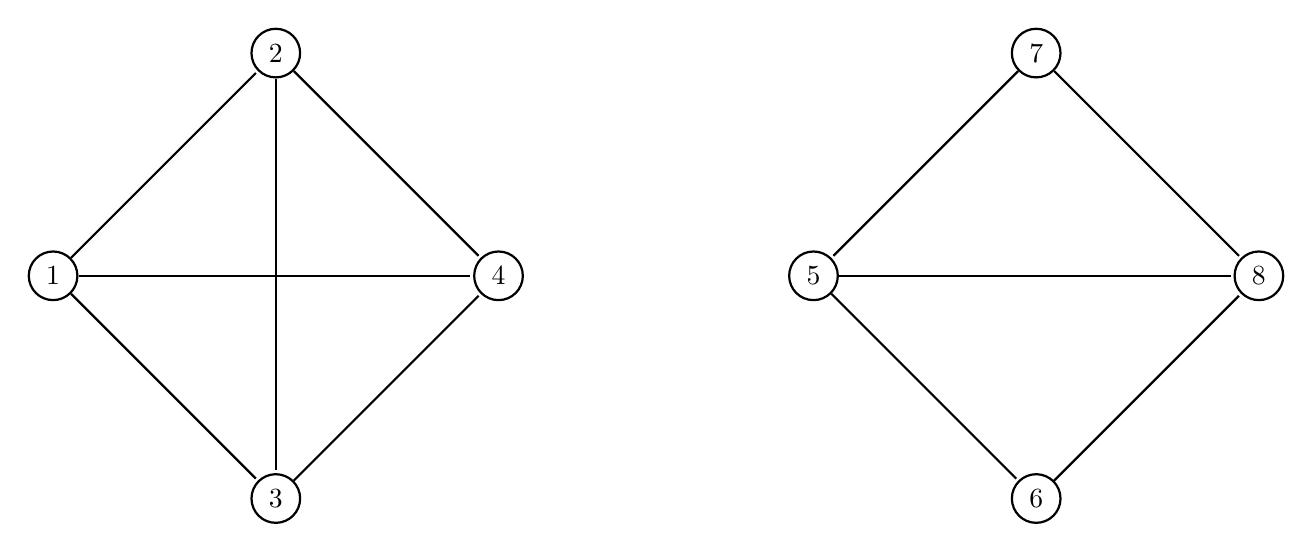
\begin{tikzpicture}[-,>=stealth',shorten >=1pt,auto,node distance=4cm, thick,main node/.style={circle,draw}, every loop/.style={}]
      \node[main node] (1) {1};
      \node[main node] (2) [above right of=1] {2};
      \node[main node] (3) [below right of=1] {3};
      \node[main node] (4) [above right of=3] {4};
      \node[main node] (5) [right of=4] {5};
      \node[main node] (6) [below right of=5] {6};
      \node[main node] (7) [above right of=5] {7};
      \node[main node] (8) [below right of=7] {8};
      \path[every node/.style={font=\sffamily\small}]
      (1) edge node {} (2)
      (1) edge node {} (3)
      (1) edge node {} (4)
      (2) edge node {} (4)
      (3) edge node {} (4)
      (2) edge node {} (3)
      (7) edge node {} (5)
      (5) edge node {} (6)
      (6) edge node {} (8)
      (7) edge node {} (8)
      (5) edge node {} (8);
      \end{tikzpicture}}
  \end{center}
  \end{definition}

  \begin{theorem}
  \[CLIQUE \leq_p ISET \text{ and } ISET \leq_p CLIQUE\]
  \end{theorem}

  \begin{definition}
  A \textbf{dominating set} in a graph $G = (V, E)$ is a subset $S \subset V$ of vertices such that for every $u \in V \setminus S$ is a neighbor in $G$ 
  \end{definition}

  \subsubsection{Anatomy of a Reduction}
  A reduction from problem $F$ to a problem $G$ is an algorithm that maps an input $x$ for $F$ to an input $R(x)$ for $G$. To show that the reduction is correct we need to show the properties of: 
  \begin{enumerate}
      \item \textit{efficiency}: algorithm $R$ runs in polynomial time
      \item \textit{completeness}: if $F(x) = 1$, then $G(R(x)) = 1$ 
      \item \textit{soundness}: if $F(R(x)) = 1$, then $G(x) = 1$
  \end{enumerate}
  Therefore, proving that problem $G$ is a reduction of problem $F$ is equivalent to showing the three properties above. 

  We finally reduce the 3SAT problem to the longest path problem. 

  \begin{theorem}[Hardness of Longest Path]
  \[3SAT \leq_p LONGPATH\]
  \end{theorem}
  That is, an efficient algorithm for the \textit{longest path} problem would imply a polynomial-time algorithm for 3SAT. Therefore, we have shown that 3SAT is no harder than Quadratic Equations, Independent Set, Maximum Cut, and Longest Path. 

\section{NP, NP Completeness, and Cook-Levin Theorem}

  All of the problems that we have talked about are \textit{search problems}, where the goal is to decide, given an instance $x$, whether there exists a solution $y$ that satisfies some condition that can verified in polynomial time. For example, in 3SAT, the instance is a formula and the solution is an assignment to the variable; in Max-Cut the instance is a graph and the solution is a cut in the graph; and so on and so forth. It turns out that every such search problem can be reduced to 3SAT. 

  \subsection{The Class NP}
  Intuitively, the class \textbf{NP} corresponds to the class of problems where it is \textit{easy to verify} a solution (i.e. verification can be done by a polynomial-time algorithm). For example, finding a satisfying assignment to a 2SAT or 3SAT formula is such a problem, since if we are given an assignment to the variables of a 2SAT or 3SAT formula then we can efficiently verify that it satisfies all constraints. 

  That is, a Boolean function $F$ is in \textbf{NP} if $F$ has the form that on input string $x$, $F(x) = 1$ if and only if there exists a "solution" string $w$ such that the pair $(x, w)$ satisfies some polynomial-time checkable condition. 

  \begin{definition}[NP - Nondeterministic Polynomial Time]
  We say that $F: \{0,1\}^* \longrightarrow \{0,1\}$ is in \textbf{NP} if there exists some integer $a > 0$ and $V: \{0,1\}^* \longrightarrow \{0,1\}$ such that $V \in \mathbf{P}$ and for every $x \in \{0,1\}^n$, 
  \[F(x) = 1 \iff \text{ there exists } w \in \{0,1\}^{n^a} s.t. \; V(x w) = 1\]
  That is, for $F$ to be in \textbf{NP}, there needs to exist some polynomial time computable verification function $V$ such that if $F(x) = 1$, then there must exist $w$ (of length polynomial in $|x|$) such that $V(x w) = 1$, and if $F(x) = 0$ then for \textit{every} such $w$, $V(xw) = 0$. Since the existence of this string $w$ certifies that $F(x) = 1$, $w$ is often called the \textit{certificate, witness}, or \textit{proof} that $F(x) = 1$. 
  \end{definition}

  Some problems that are NP are: 
  \begin{enumerate}
      \item $3SAT \in \mathbf{NP}$ since for every $l$-variable formula $\varphi$, $3SAT(\varphi) = 1$ if and only there exists a satisfying assignment $x \in \{0,1\}^l$ such that $\varphi(x) = 1$, and we can check this condition in polynomial time. 
      \item $QUADEQ \in \mathbf{NP}$ since for every $l$-variable instance of quadratic equations $E$, $QUADEQ (E) = 1$ if and only if there exists an assignment $x \in \{0,1\}^l$ that satisfies $E$. We can check the condition that $x$ satisfies $E$ in polynomial time by enumerating over all the equations in $E$, and for each such equation $e$, plug in the values of $x$ and verify that $e$ is satisfied. 
      \item $ISET \in \mathbf{NP}$ since for every graph $G$ and integer $k$, $ISET(G, k) = 1$ if and only if there exists a set $S$ of $k$ vertices that contains no pair of neighbors in $G$. We can check the condition that $S$ is an independent set of size $\geq k$ in polynomial time by first checking that $|S| \geq k$ and then enumerating over all edges $\{u, v\}$ in $G$, and for each such edge verify that either $u \neq S$ or $v \neq S$. 
      \item $LONGPATH \in \mathbf{NP}$ since for every graph $G$ and integer $k$, $LONGPATH(G, k) = 1$ if and only if there exists a simple path $P$ in $G$ that is of length at least $k$. We can check the condition that $P$ is a simple path of length $k$ in polynomial time by checking that it has the form $(v_0, v_1, ..., v_k)$ where each $v_i$ is a vertex in $G$, no $v_i$ is repeated, and for every $i \in [k]$, the edge $\{v_i, v_{i+1}\}$ is present in the graph. 
      \item $MAXCUT \in \mathbf{NP}$ since for every graph $G$ and integer $k$, $MAXCUT (G, k) = 1$ if and only if there exists a cut $(S, \overline{S})$ in $G$ that cuts at least $k$ edges. We can check that condition that $(S, \overline{S})$ is a cut of value at least $k$ in polynomial time by checking that $S$ is a subset of $G$'s vertices and enumerating over all the edges $\{u, v\}$ of $G$, counting those edges such that $u \in S$ and $v \not\in S$ or vice versa. 
  \end{enumerate}

  \begin{theorem}
  Verifying is no harder than solving: 
  \[\mathbf{P} \subseteq \mathbf{NP}\]
  Furthermore, 
  \[\mathbf{P} \subseteq \mathbf{NP} \subseteq \mathbf{EXP}\]
  \begin{center}
  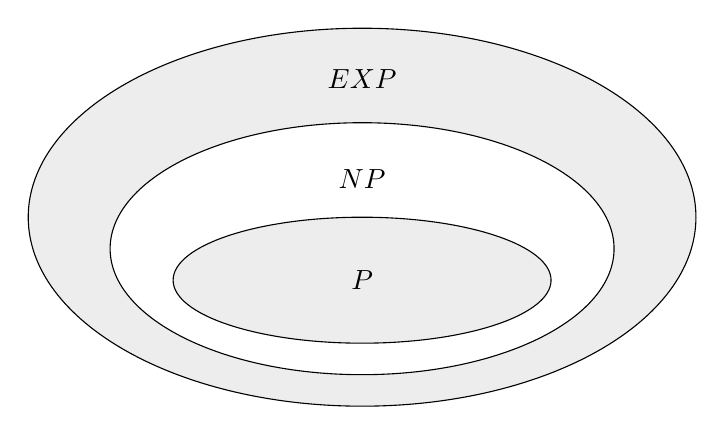
\begin{tikzpicture}[scale=0.8]
      \draw[fill=lightgray] (0,1) ellipse (5.3 and 3);
      \draw[fill=white] (0,0.5) ellipse (4 and 2);
      \draw[fill=lightgray] (0,0) ellipse (3 and 1);
      \node at (0,0) {$P$};
      \node at (0,1.6) {$NP$};
      \node at (0,3.2) {$EXP$};
  \end{tikzpicture}
  \end{center}
  \end{theorem}
  \begin{proof}
  Suppose that $F \in \mathbf{P}$. Define the following function $V$:
  \[V (x 0^n) = \begin{cases}
  1 & \text{iff } n = |x|, F(x) = 1 \\
  0 & \text{else} 
  \end{cases}\]
  Since $F \in \mathbf{P}$, we can clearly compute $V$ in polynomial time as well. Let $x \in \{0,1\}^n$ be some string. If $F(x) = 1$ then $V(x 0^n) = 1$. On the other hand, if $F(x) = 0$ then for every $w \in \{0,1\}^n$, $V(xw) = 0$. Therefore, setting $a = 1$ (i.e. $w \in \{0,1\}^{n^1}$), we see that $V$ satisfies the NP condition. 
  \end{proof}

  \subsection{NP Hard and NP Complete Problems}
  There are countless examples of problems for which we do not know if their best algorithm is polynomial or exponential, but we can show that they are in \textbf{NP}; that is, we don't know if they are easy to \textit{solve}, but we do know that it is easy to \textit{verify} a given solution. There are many other functions that we would like to compute that are easily shown to be in \textbf{NP}. In fact, it we can solve 3SAT then we can solve all of them! 

  \begin{theorem}[Cook-Levin Theorem]
  For every $F \in \mathbf{NP}$, 
  \[F \leq_p 3SAT\]
  \end{theorem}
  This immediately implies that $QUADEQ, LONGPATH$, and $MAXCUT$ (and really, \textit{every} $F \in \mathbf{NP}$) all reduce to $3SAT$, meaning that all these problems are equivalent! All of these problems are the "hardest in \textbf{NP}" since an efficient algorithm for any one of them would imply an efficient algorithm for \textit{all} the problems in \textbf{NP}. 

  \begin{definition}
  Let $G: \{0,1\}^* \longrightarrow \{0,1\}$. We say that $G$ is \textbf{NP hard} if for every $F \in \mathbf{NP}$, $F \leq_p G$. We say that $G$ is \textbf{NP complete} if $G$ is \textbf{NP} hard and $G \in \mathbf{NP}$. 
  \end{definition}

  Therefore, despite their differences, 3SAT, quadratic equations, longest path, independent set, maximum cut, and thousands of other problems are all \textbf{NP} complete. Again, this means that \textit{if a single \textbf{NP} complete problem has a polynomial-time algorithm, then there is such a polynomial-time algorithm for every decision problem that corresponds to the existence of an efficiently verifiable solution (i.e. is NP), which would imply that \textbf{P = NP}}.

  \subsection{P = NP?}
  However, a polynomial-time algorithm for even a single one of the \textbf{NP} complete problems has even been found, proving support that \textbf{P $\neq$ NP}

  One of the mysteries of computation is that people have observed a certain empirical “zero-one law” or “dichotomy” in the computational complexity of natural problems, in the sense that many natural problems are either in \textbf{P} (often in $TIME(O(n))$ or $TIME(O(n^2))$), or they are \textbf{NP} hard. This is related to the fact that for most natural problems, the best known algorithm is either exponential or polynomial, rather than any strange function in between. 

  However, it is believed that there exist problems in \textbf{NP} that are neither in \textbf{P} nor are \textbf{NP} complete, and in fact a result known as \textbf{Lander's Theorem} shows that if $\mathbf{P \neq NP}$, then this is indeed the case. Therefore, we are left with two cases:
  \begin{enumerate}
      \item If $\mathbf{P} \neq \mathbf{NP}$, meaning that \textbf{P} is a strict subset of \textbf{NP} and by Lander's theorem, \textbf{NP} complete problems do not cover all of $\mathbf{NP} \setminus \mathbf{P}$. (left)
      \item If $\mathbf{P} = \mathbf{NP}$, meaning that $\mathbf{P} = \mathbf{NP} = \mathbf{NP}$ complete. (right)
  \end{enumerate}
  \begin{center}
  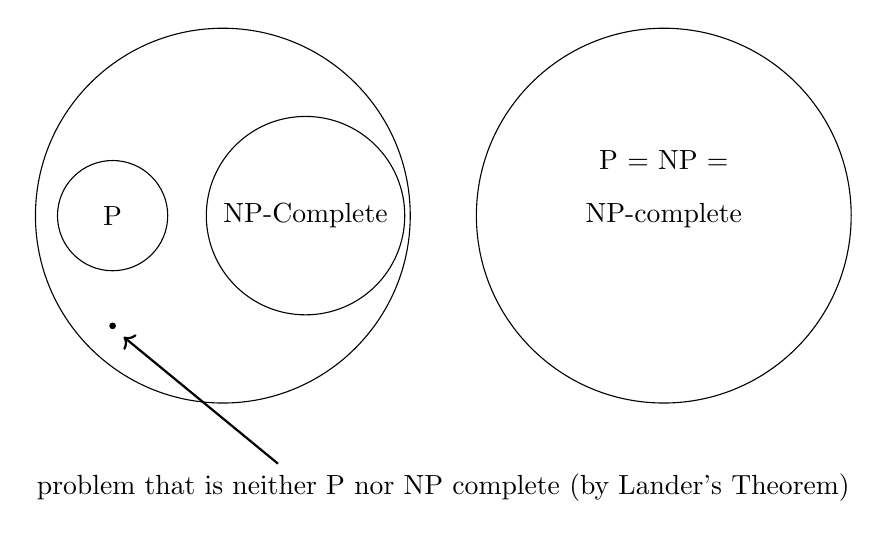
\begin{tikzpicture}[scale=0.7]
      \draw (-4, 0) circle (3.4);
      \draw (4, 0) circle (3.4);
      \draw (-6, 0) circle (1);
      \node at (-6,0) {P};
      \draw (-2.5, 0) circle (1.8);
      \node at (-2.5,0) {NP-Complete};
      \node at (4, 1) {P = NP = };
      \node at (4, 0) {NP-complete};
      \draw[fill] (-6, -2) circle (0.05);
      \draw[->, thick] (-3, -4.5)--(-5.8,-2.2);
      \node[below] at (0, -4.5) {problem that is neither P nor NP complete (by Lander's Theorem)};
  \end{tikzpicture}
  \end{center}

  \subsection{NANDSAT, 3NAND Problems}
  \begin{definition}
  The function $NANDSAT: \{0,1\}^* \longrightarrow \{0,1\}$ is defined as follows: 
  \begin{enumerate}
      \item The input to $NANDSAT$ is a string $Q$ representing a NAND-CIRC program (or equivalently, a circuit with $NAND$ gates)
      \item The output of $NANDSAT$ on input $Q$ is $1$ if and only if there exists a string $w \in \{0,1\}^n$ (where $n$ is the number of inputs to $Q$) such that $Q(w) = 1$. 
  \end{enumerate}
  \end{definition}

  \begin{definition}
  The $3NAND$ problem is defined as follows: 
  \begin{enumerate}
      \item The input is a logical formula $\Psi$ on a set of variables $z_0, ..., z_{r-1}$ which is an AND of constraints of the form $z_i = NAND(z_j, z_k)$. 
      \item The output is $1$ is and only if there is an input $z \in \{0, 1\}^r$ that satisfies all of the constraints. 
  \end{enumerate}
  \end{definition}

  \begin{example}
  The following is a $3NAND$ formula with $5$ variables and $3$ constraints:
  \[\Psi = \big( z_3 = NAND(z_0, z_2)\big) \wedge \big( z_1 = NAND(z_0, z_2)\big) \wedge \big( z_4 = NAND(z_3, z_1)\big)\]
  In this case $3NAND(\Psi) = 1$, since the assignment $z = 01010$ satisfies it. Given a $3NAND$ formula $\Psi$ of $r$ variables and an assignment $z \in \{0,1\}^r$, we can check in polynomial time whether $\Psi (z) = 1$, and hence $3NAND \in \mathbf{NP}$. 
  \end{example}

  \begin{theorem}
  $NANDSAT$ and $3NAND$ is \textbf{NP} complete. 
  \end{theorem}

\section{Probabilistic Computation}

  It turns out that randomness can actually be a resource for computation, enabling us to achieve tasks much more efficiently than previously known. This advantage comes from the idea that calculating the statistics of a system could be done much faster by running several randomized simulations rather than explicit calculations, and these types of randomized algorithms are known as \textit{Monte Carlo algorithms}. 

  \subsection{Finding Approximately Good Maximum Cuts}
  Recall the maximum cut problem of finding, given a graph $G = (V, E)$, the cut that maximizes the number of edges. This problem is \textbf{NP}-hard, which means that we do not know of any efficient algorithm that can solve it, but randomization enables a simple algorithm that can cut at least half of the edges. 

  \begin{theorem}[Approximating Max Cut]
  There is an efficient probabilistic algorithm that on input an $n$-vertex $m$-edge graph $G$, outputs a cut $(S, \overline{S})$ that cuts at least $m/2$ of the edges of $G$ in expectation. 
  \end{theorem}
  \begin{proof}
  We simply choose a \textit{random cut}: we choose a subset $S$ of vertices by choosing every vertex $v$ to be a member of $S$ with probability $1/2$ independently. More specifically, upon input of a graph $G = (V, E)$ with vertices $(v_0, ..., v_{n-1})$, we do
  \begin{enumerate}
      \item Pick $x$ uniformly at random in $\{0,1\}^n$
      \item Let $S \subseteq V$ be the set $\{v_i \;|\; x_i = 1, i \in [n]\}$ that includes all vertices corresponding to coordinates of $x$ where $x_i = 1$. 
      \item Output the cut $(S, \overline{S})$. 
  \end{enumerate}
  \end{proof}

  We claim that the expected number of edges cut by the algorithm is $m/2$. Indeed, for every edge $e \in E$, let $X_e$ be the random variable such that $X_e (x) = 1$ if the edge is cut by $x$, and let $X_e (x) = 0$ otherwise. It is not hard to see that the probability of $X_e (x) = 1$ is $\frac{1}{2}$ (when exactly one of the vertices are in $S$), and hence 
  \[\mathbb{E} (X_e) = 1/2\]
  Summing this over all edges and by linearity of expectation, we get
  \[\mathbb{E}(X) = \sum_{e \in E} \mathbb{E}(X_e) = m \cdot \frac{1}{2} = \frac{m}{2}\]
  In fact, for \textit{every graph $G$}, the algorithm is guaranteed to cut half of the edges of the input graph in expectation. 

  \subsubsection{Amplifying the success of randomized algorithms}
  But note that expectation does not imply concentration. Luckily, we can \textit{amplify} the probability of success by repeating the process several times and outputting the best cut we find. We assume that the probability that the algorithm above succeeds in cutting at least $m/2$ edges is not \textit{too} tiny. 

  \begin{lemma}
  The probability that a random cut in an $m$ edge graph cuts at least $m/2$ edges is at least $\frac{1}{2m}$. 
  \end{lemma}
  \begin{proof}
  This is quite trivial when looking at specific cases. For example, take the case when $m =1000$ edges. In this case, one can shot that we will cut at least 500 edges with probability at least $0.001$ (and so in particular larger then $\frac{1}{2m} = \frac{1}{2000}$). Specifically, if we assume otherwise, then this means that with probability more than $0.999$ the algorithm cuts $499$ or fewer edges. But since we can never cut more than the total of $1000$ edges, given this assumption, the highest value of the expected number of edges cut is if we cut exactly $499$ edges with probability $0.999$ and cut $1000$ edges with probability $0.001$. But this leads to the expectation being
  \[0.999 \cdot 499 + 0.001 \cdot 1000 < 500\]
  which contradicts the fact that the expectation to be at least $500$ in the previous theorem. Generalizing this to $m$ edges, we find that the expected number of edges cut is 
  \[pm + (1-p) \Big( \frac{m}{2} - \frac{1}{2} \Big) \leq pm + \frac{m}{2} - \frac{1}{2}\]
  But since $p < \frac{1}{2m} \implies pm < 0.5$, the right hand side is smaller than $m/2$, contradicting the fact that the expected number of edges cut is at least $m/2$. 
  \end{proof}

  \subsubsection{Success Amplification}
  To increase the chances of success, we simply need to repeat our program many times, with fresh randomness each time, and output the best cut we get in one of these repetitions. It turns our that if we repeat this experiment $2000m$ times, then by using the inequality
  \[\Big( 1 - \frac{1}{k} \Big)^k \leq \frac{1}{e} \leq \frac{1}{2}\]
  we can show that the probability that we will never cut at least $m/2$ edges is at most 
  \[\Big( 1 - \frac{1}{2m} \Big)^{2000m} \leq 2^{-1000}\]

  This can be generalized in the following lemma. 

  \begin{lemma}
  There is an algorithm that on input graph $G = (V, E)$ and a number $k$, runs in polynomial time in $|V|$ and $k$ and outputs a cut $(S \overline{S})$ such that
  \[\mathbb{P}\Big(\text{number of edges cut by } (S, \overline{S}) \geq \frac{|E|}{2} \Big) \geq 1 - 2^{-k}\]
  \end{lemma}
  \begin{proof}
  Just repeat the previous algorithm $200km$ times and compute the probability of failure. 
  \end{proof}

  \subsubsection{Two-sided Amplification}
  The analysis above relied on the fact that the maximum has \textit{one sided error}; that is, if we get a cut of size at least $m/2$ then we know we have succeeded. This is common for randomized algorithms, but it is not the only case. In particular, consider the task of computing some Boolean function $F: \{0,1\}^* \longrightarrow \{0,1\}$. A randomized algorithm $A$ for computing $F$, given input $x$, might toss coins and succeed in outputting $F(x)$ with probability, say $0.9$. We say that $A$ has \textit{two sided errors} if there is a positive probability that $A(x)$ outputs $1$ when $F(x) = 0$ and positive probability that $A(x)$ outputs $0$ when $F(x) = 1$. So, we cannot simply repeat it $k$ times and output $1$ if a single one of those repetitions resulted in $1$, nor can we output $0$ if a single one of the repetitions resulted in $0$. But we can output the \textit{majority value} of these repetitions: the probability that the fraction of the repetitions where $A$ will output $F(x)$ will be at least, say $0.89$, will be exceptionally close to $1$ and in such cases we will output the correct answer. 

  \begin{theorem}
  If $F: \{0,1\}^* \longrightarrow \{0,1\}$ is a function such that there is a polynomial-time algorithm $A$ satisfying 
  \[\mathbb{P} \big( A(x) = F(x) \big) \geq 0.51\]
  for every $x \in \{0,1\}^*$, then there is a polynomial time algorithm $B$ satisfying
  \[\mathbb{P} \big( B(x) = F(x) \big) \geq 1 - 2^{-|x|}\]
  for every $x \in \{0,1\}^*$. 
  \end{theorem}

  \subsubsection{Solving SAT through Randomization}
  The 3SAT problem is \textbf{NP} hard, and so it is unlikely that it has a polynomial (or even subexponential) time algorithm. But this does not mean that we can't do at least somewhat better than the trivial $2^n$ algorithm for $n$-variable 3SAT. The best known worst-case algorithms are randomized and are at their base the following simple algorithm. In this algorithm, called \textit{WalkSAT}, the input is an $n$ variable 3CNF formula $\varphi$, the parameters are any numbers $T, S \in \mathbb{N}$, and the operation is: 
  \begin{enumerate}
      \item Repeat the following $T$ steps: 
      \begin{enumerate}
          \item Choose a random assignment $x \in \{0,1\}^n$ and repeat the following for $S$ steps: 
          \begin{enumerate}
              \item If $x$ satisfies $\varphi$, then output $x$. 
              \item Otherwise, choose a random clause $(l_i \vee l_j \vee l_k)$ that $x$ does not satisfy, choose a random literal in $l_i \vee l_j \vee l_k$ and modify $x$ to satisfy this literal. 
          \end{enumerate}
      \end{enumerate}
      \item If all the $T \cdot S$ repetitions above did not result in a satisfying assignment, then output $\texttt{Unsatisfiable}$. 
  \end{enumerate}
  Note that we are only going though at most $S\cdot T$ configurations of $x \in \{0,1\}^n$, and the running time of this algorithm is $S \cdot T \cdot poly(n)$. The fact that this algorithm is efficient is taken care of, so now the key question is how small we can make $S$ and $T$ so that the probability that WalkSAT outputs $\texttt{Unsatisfiable}$ on a satisfiable formula $\varphi$ is small. It is known that we can do with 
  \[ST = \Tilde{O} \big( (4/3)^n \big) = \Tilde{O} ( 1.\overline{3}^n)\]
  However, we will prove a weaker bound in the following theorem (which is still much better than the $2^n$ bound). 

  \begin{theorem}[WalkSAT simple analysis]
  If we set $T = 100\sqrt{3}^n$ and $S = n/2$, then the probability we output $\texttt{Unsatisfiable}$ for a satisfiable $\varphi$ is at most $\frac{1}{2}$. 
  \end{theorem}

  \subsubsection{Bipartite Matching}

  \begin{definition}
  A \textbf{bipartite graph} $G = (L \cup R, E)$ has $2n$ vertices partitioned into $n$-sized sets $L$ and $R$, where all edges have one endpoint in $L$ and the other in $R$.
  \begin{center}
      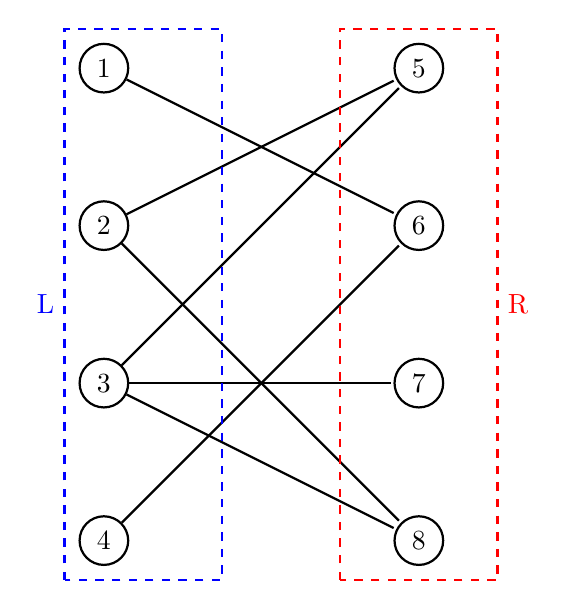
\begin{tikzpicture}[-,>=stealth',shorten >=1pt,auto,node distance=2cm, thick,main node/.style={circle,draw}, every loop/.style={}]
      \node[main node] (1) {1};
      \node[main node] (2) [below of=1] {2};
      \node[main node] (3) [below of=2] {3};
      \node[main node] (4) [below of=3] {4};
      \node[main node] (a) [right of=1] {a};
      \node[main node] (5) [right of=a] {5};
      \node[main node] (6) [below of=5] {6};
      \node[main node] (7) [below of=6] {7};
      \node[main node] (8) [below of=7] {8};
      \path[every node/.style={font=\sffamily\small}]
      (1) edge node {} (6)
      (2) edge node {} (5)
      (2) edge node {} (8)
      (3) edge node {} (5)
      (3) edge node {} (7)
      (3) edge node {} (8)
      (4) edge node {} (6);
      \draw[fill=white, white] (1.5, -0.5) rectangle (2.5, 0.5);
      \draw[dashed, blue] (-0.5, -6.5) rectangle (1.5, 0.5);
      \draw[dashed, red] (3, -6.5) rectangle (5, 0.5);
      \node[left, blue] at (-0.5,-3) {L};
      \node[right, red] at (5, -3) {R};
      \end{tikzpicture}
  \end{center}
  \end{definition}
  A \textit{matching problem} is a type of problem where we match nodes to each other with edges. One variant of it is called the \textit{bipartite perfect matching}. The goal is to determine whether there is a \textit{perfect matching}, a subset $M \subseteq E$ of $n$ disjoint edges that connects every vertex $L$ to a unique vertex in $R$. 

  It turns out that by reducing this problem of finding a matching in $G$ to finding a maximum flow (or equivalently, a minimum $s, t$ cut) in a related graph $G^\prime$ (below), we can solve it in polynomial time. 
  \begin{center}
      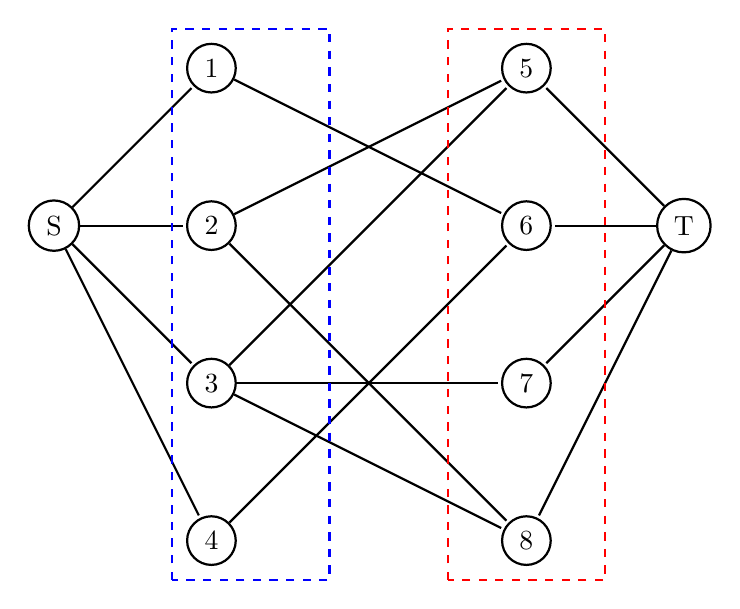
\begin{tikzpicture}[-,>=stealth',shorten >=1pt,auto,node distance=2cm, thick,main node/.style={circle,draw}, every loop/.style={}]
      \node[main node] (1) {1};
      \node[main node] (2) [below of=1] {2};
      \node[main node] (3) [below of=2] {3};
      \node[main node] (4) [below of=3] {4};
      \node[main node] (a) [right of=1] {a};
      \node[main node] (5) [right of=a] {5};
      \node[main node] (6) [below of=5] {6};
      \node[main node] (7) [below of=6] {7};
      \node[main node] (8) [below of=7] {8};
      \node[main node] (S) [left of=2] {S};
      \node[main node] (T) [right of=6] {T};
      \path[every node/.style={font=\sffamily\small}]
      (1) edge node {} (6)
      (2) edge node {} (5)
      (2) edge node {} (8)
      (3) edge node {} (5)
      (3) edge node {} (7)
      (3) edge node {} (8)
      (4) edge node {} (6)
      (S) edge node {} (1)
      (S) edge node {} (2)
      (S) edge node {} (3)
      (S) edge node {} (4)
      (T) edge node {} (5)
      (T) edge node {} (6)
      (T) edge node {} (7)
      (T) edge node {} (8);
      \draw[fill=white, white] (1.5, -0.5) rectangle (2.5, 0.5);
      \draw[dashed, blue] (-0.5, -6.5) rectangle (1.5, 0.5);
      \draw[dashed, red] (3, -6.5) rectangle (5, 0.5);
      \end{tikzpicture}
  \end{center}
  However, there is a different probabilistic algorithm to do this. Let $G$'s vertices be labeled as $L = \{l_0, ..., l_{n-1}\}$ and $R = \{r_0, ..., r_{n-1}\}$. A matching $M$ corresponds to a \textit{permutation} $\pi \in S_n$ where for ever $i \in [n]$, we define $\pi(i)$ to be the unique $j$ such that $M$ contains the edge $\{l_i, r_j\}$. Define an $n \times n$ matrix $A = A(G)$ where $A_{i, j} = 1$ if and only if $\{l_i, r_j\}$ is present and $A_{i, j} = 0$ otherwise. The correspondence between matchings and permutations implies the following claim. 

  \begin{lemma}[Matching polynomial]
  Define $P = P(G)$ to be the polynomial mapping $\mathbb{R}^{n^2}$ to $\mathbb{R}$ where 
  \[P(x_{0, 0}, ..., x_{n-1, n-1} = \sum_{\pi \in S_n} \bigg( \prod_{i=0}^{n-1} sign(\pi) A_{i, \pi(i)} \bigg) \prod_{i=0}^{n-1} x_{i, \pi(i)}\]
  In fact, given the matrix $A$ representing the graph, the polynomial above is the determinant of the matrix $A(x)$, which is obtained by replaying $A_{i, j}$ with $A_{i, j} x_{i, j}$. Then $G$ has a perfect matching if and only if $P$ is not identically zero (i.e. if there exists some assignment $x = (x_{i, j})_{i, j \in [n]} \in \mathbb{R}^{n^2}$ such that $P(x) \neq 0$. 
  \end{lemma}
  This reduces testing perfect matching to testing whether a given polynomial $P(\cdot)$ is identically $0$ or not. The kernel of most multivariate nonzero polynomials form a strictly lower dimensional space than the total space, so in order to do this, we just choose a "random" input $x$ and check if $P(x) \neq 0$. However, to transform this into an actual algorithm, we can't work in the real numbers with our finite computational power. We use the following. 

  \begin{theorem}[Schwartz-Zippel Lemma]
  For every integer $q$ and polynomial $P: \mathbb{R}^n \longrightarrow \mathbb{R}$ with integer coefficients, if $P$ has degree at most $d$ and is not identically zero, then it has at most $d q^{n-1}$ roots in the set 
  \[[q]^n = \big\{(x_0, ..., x_{n-1}) \;|\; x_i \in \{0, 1, ..., q-1\}\big\}\]
  \end{theorem}

  Therefore, upon an input of a bipartite graph $G$ on $2n$ vertices $\{l_0, ..., l_{n-1}, r_0, ..., r_{n-1}\}$, the \textit{Perfect-Matching algorithm} can be divided into these steps: 
  \begin{enumerate}
      \item For every $i, j \in [n]$, choose $x_{i, j}$ independently at random from $[2n] = \{0, ..., 2n-1\}$. 
      \item Compute the determinant of the matrix $A(x)$ whose $i, j$th entry equals $x_{i, j}$ if the edge $\{l_i, r_j\}$ is present and $0$ otherwise. 
      \item Output $\texttt{no perfect matching}$ if determinant is $0$, and output $\texttt{perfect matching}$ otherwise. 
  \end{enumerate}

\section{Modeling Randomized Computation}

  While we have described randomized algorithms in an informal way, we haven't addressed two questions: 
  \begin{enumerate}
      \item How do we actually efficiently obtain random strings in the physical world? 
      \item What is the mathematical model for randomized computations, and is it more powerful than deterministic computation? 
  \end{enumerate}
  The first question is important, but we will assume that there are various physical sources of random or unpredictable data, such as a user's mouse movements, network latency, thermal noise, and radioactive decay. For example, many Intel chips come with a random number generator built in. We will focus on the second question. 

  \subsection{Modeling Randomized Computation}
  Modeling randomized computation is actually quite easy. We can add the operation
  \[\texttt{foo = RAND()}\]
  in addition to things like the NAND operator to any programming language such as NAND-TM, NAND-RAM, NAND-CIRC, etc., where $\texttt{foo}$ is assigned to a random bit in $\{0,1\}$ independently every time it is called. These are called RNAND-TM, RNAND-RAM, and RNAND-CIRC, respectively. 

  Similarly, we can easily define randomized Turing machines as Turing machines in which the transition function $\delta$ gets an extra input (in addition to the current state and symbol read from the tape) a bit $b$ that in each step is chosen at random in $\{0, 1\}$. Of course the function can ignore this bit (and have the same output regardless of whether $b = 0$ or $b= 1$) and hence randomized Turing machines generalize deterministic Turing machines. 

  We can use the $\texttt{RAND()}$ operation to define the notion of a function being computed by a randomized $T(n)$ time algorithm for every nice time bound $T: \mathbb{N} \longrightarrow \mathbb{N}$, but we will only define the class of functions that are computable by randomized algorithms running in \textit{polynomial time}. 

  \begin{definition}[The class \textbf{BPP}]
  Let $F: \{0, 1\}^* \longrightarrow \{0,1\}$. We say that $F \in \mathbf{BPP}$ if there exist constants $a, b \in \mathbb{N}$ and a RNAND-TM program $P$ such that for every $x \in \{0,1\}^*$, on input $x$, the program $P$ halts within at most $a |x|^b$ steps and 
  \[\mathbb{P} \big(P(x) = F(x)\big) \geq \frac{2}{3}\]
  where this probabilty is taken over the result of the RAND operations of $P$. Note that this probability is taken only over the random choices in the execution of $P$ and \textit{not} over the choice of the input $x$. That is, \textbf{BPP} is still a \textit{worst case} complexity class, in the sense that if $F$ is in \textbf{BPP} then there is a polynomial-time randomized algorithm that computes $F$ with probability at least $2/3$ on \textit{every possible} (and not just random) input. 
  \end{definition}

  We will use the name \textit{polynomial time randomized algorithm} to denote a computation that can be modeled by a polynomial-time RNAND-TM program, RNAND-RAM program, or a randomized Turing machine. 

  Alternatively, we can think of a randomized algorithm $A$ as a \textit{deterministic algorithm} $A^\prime$ that takes two inputs $x$ and $r$ where the input $r$ is chosen at random from $\{0, 1\}^m$ for some $m \in \mathbb{N}$. The equivalence to the previous definition is shown in the following theorem: 

  \begin{definition}[Alternative characterization of \textbf{BPP}]
  Let $F: \{0, 1\}^* \longrightarrow \{0, 1\}$. Then $F \in \mathbf{BPP}$ if and only if there exists $a, b \in \mathbb{N}$ and $G: \{0, 1\}^* \longrightarrow \{0, 1\}$ such that $G$ is in $\mathbf{P}$ and for every $x \in \{0, 1\}^*$, 
  \[\mathbb{P}\big( G(xr) = F(x)\big) \geq \frac{2}{3}\]
  where $r$ is chosen at random from $\{0, 1\}^{a|x|^b}$. As such, if $A$ is a randomized algorithm that on inputs of length $n$ makes at most $m$ coin tosses, we will often use the notation $A(x; r)$ (where $x \in \{0, 1\}^n$ and $r \in \{0, 1\}^m$ to refer to the result of executing $x$ when the coin tosses of $A$ correspond to the coordinates of $r$. This second input $r$ is sometimes called a \textbf{random tape}.
  \end{definition}

  The relationship between \textbf{BPP} and \textbf{NP} is not known, but we do know the following. 

  \begin{theorem}[Sipser-Gacs Theorem]
  If $\mathbf{P = NP}$ then $\mathbf{BPP = P}$. 
  \end{theorem}

  \subsubsection{Success Amplification of two-sided error algorithms}
  The number $2/3$ may seem arbitrary, but it can be amplified to our liking.

  \begin{theorem}[Amplification]
  Let $F: \{0, 1\}^* \longrightarrow \{0, 1\}$ be a Boolean function such that there is a polynomial $p: \mathbb{N} \longrightarrow \mathbb{N}$ and a polynomial-time randomized algorithm $A$ satisfying that for every $x \in \{0, 1\}^n$, 
  \[\mathbb{P} \big( A(x) = F(x) \big) \geq \frac{1}{2} + \frac{1}{p(n)}\]
  Then for every polynomial $q: \mathbb{N} \longrightarrow \mathbb{N}$, there is a polynomial-time randomized algorithm $B$ satisfying for every $x \in \{0, 1\}^n$,
  \[\mathbb{P} \big( B(x) = F(x)\big) \geq 1 - 2^{-q(n)}\]
  \end{theorem}

  \subsubsection{BPP and NP Completeness}
  The theory of \textbf{NP} completeness still applies to probabilistic algorithms. 

  \begin{theorem}
  Suppose that $F$ is \textbf{NP} hard and $F \in \mathbf{BPP}$. Then 
  \[\mathbf{NP \subseteq BPP}\]
  That is, if there was a randomized polynomial time algorithm for any \textbf{NP} complete problem such as 3SAT, ISET, etc., then there would be such an algorithm for \textit{every} problem in \textbf{NP}. 
  \end{theorem}

  \subsection{The Power of Randomization}
  To find out whether randomization can add power to computation (does \textbf{BPP=P}?), we prove a few statements about the relationship of \textbf{BPP} with other complexity classes. 

  \begin{theorem}[Simulating randomized algorithms in exponential time]
  \[\mathbf{BPP \subseteq EXP}\]
  \end{theorem}
  \begin{proof}
  We can just enumerate over all the (exponentially many) choices for the random coins. 
  \end{proof}

  Furthermore, 
  \[\mathbf{P \subseteq BPP \subseteq EXP}\]

\end{document}
